%%%%%%%%%%%%%%%%%%%%%%%%%%%%%%%%%%%%%%%%%%%
% Template for Doctoral Theses at Uppsala %
% University. The template is based on    %
% the layout and typography used for      %
% dissertations in the Acta Universitatis %
% Upsaliensis series                      %
% Ver 4.0.1 - 2008-11-03                  %
%                                         %
% Publishing & Graphic Services           %
% espik@ub.uu.se                          %
%                                         %
%%%%%%%%%%%%%%%%%%%%%%%%%%%%%%%%%%%%%%%%%%%


\documentclass[11pt,a4paper,twoside, openright]{book} % Default font 11pt, A4, all pages are printed the same, new chapter always begins on a right-hand page.

% Package import
% Language, diacritics and hyphenation
\usepackage[swedish,english]{babel} % Use English and Swedish languages. English default. English hyphenation.
\usepackage[latin1]{inputenc} % Unix users should include this package instead of ansinew or applemac for correct handling of diacritics.
%\usepackage[applemac]{inputenc} % Macintosh users should include this package instead of ansinew or latin1 for correct handling of diacritics.
%\usepackage[ansinew]{inputenc} % % Windows users should include this package instead of applemac or latin1 for correct handling of diacritics.
\usepackage[T1]{fontenc}% Enables the use of 8-bit characters and �, �, � can be typed as �, �, � instead of the corresponding commands.

% Page elements
\usepackage{mathptmx} % Default font for dissertations is Times.
%\usepackage{fourier} % If mathematics don't display well using Times, then use Fourier.
\usepackage{helvet} % Default sans-serif font.
\usepackage{courier}% Default typewriter (monotype) font.
\usepackage{Thesis} % This package is specific for theses written at Uppsala University. Modifications to the classfile and the document can be found here.
\ifpdf
   \usepackage[pdftex]{graphicx}
  \else
    \usepackage[dvips]{graphicx}
\fi % Used for figures
\usepackage{booktabs} % Produces good three line tables which is the standard tabel format for disserations.
\usepackage[colorlinks=true, urlcolor=black, pagecolor=black, linkcolor=black, citecolor=black, filecolor=black, menucolor=black, pdfpagelabels,bookmarksnumbered=true]{hyperref} % Use this package to produce links in the electronic version of the document. All hyperlinks are black. Page view is set to Fit Width and page layout is set to display the document spread.  Make page anchors using the formatted form of the page number.  Set PDF page labels; i.e., write the value of \thepage to the PDF file so that Acrobat Reader can display the page number as (say) 'ii (4 of 40)' rather than simply '4 of 40'.

\usepackage[usenames,dvipsnames,svgnames,table]{xcolor}
% Nas styles
\usepackage{nasutilsp}

% Make the first letter of a paragraph bigger, spans over multiple lines
\usepackage{lettrine}

% enumerate inline
\usepackage[inline]{enumitem}
\usepackage{subfig}
\usepackage{amsmath}
\usepackage{eucal}
\usepackage[linesnumbered,lined,boxed,commentsnumbered]{algorithm2e}
\usepackage{amsfonts}
%\usepackage{amssymb}
%\usepackage{anyfontsize}
% Bibliographic information
% Filling in this bibliographic information facilitates the
% processing of this document.
% Insert linebreaks if necessary
% The abstract page is not generated by default. The reason for this is that it
% will be generated by the unit for Publishing and Graphic sevices from the metadata 
% template ("Spikningsmallen"). If you want to include the abstract page generated from this template,
% please edit the \frontmatterMonograph or \frontmatterCS command at the en of this file
%. Because of this, some of the bibliografic data on this page will not be used.

% Abstract and titelpage
\newcommand{\authorSurname}{Mahmud} % Your surname
\newcommand{\authorFirstName}{Nesredin} % Your given name
\newcommand{\authorFirstInitial}{N} % Initial of given name
\newcommand{\authorEmail}{nesredin.mahmud@mdh.se} % Your e-mail address
\newcommand{\dissertationTitle}{Design of Assured and Efficient Safety-critical Systems using Formal Methods and Optimization Techniques} % The title of the dissertation
\newcommand{\dissertationSubtitle}{Subtitle of the dissertation}% The subtitle of the dissertation (if there is any).
\newcommand{\yearOfPublication}{2019} % Year of publication
\newcommand{\placeOfDisputation}{M\"{a}lardalen University} % Place of disputation
\newcommand{\dateOfDisputation}{Thursday, June 13, 2019} % Date of disputation (Day, Month, Year)
\newcommand{\timeOfDisputation}{13:15} % Time of disputation (Swedish time format)
\newcommand{\disputationLanguage}{English} % Language the examination will be conducted in.
\newcommand{\numberOfPages}{51} % The page number of the last page
\newcommand{\placeOfPublication}{Uppsala} % The place of publication
\newcommand{\ISBN}{978-91-554-5436-4} % The ISBN number of the dissertation.
\newcommand{\series}{Uppsala Dissertations from the Faculty of Science and Technology} % The title of the series
\newcommand{\serialNumber}{1214} % The number in the series.
\newcommand{\keywords}{ embedded system, real-time system, safety-critical system, requirements specification, formal method, Simulink, integer-linear programming, metaheuristics} % Key words separated by comma
\newcommand{\department}{Department of Electronic Publishing} % Name of your department
\newcommand{\departmentaddress}{Villavagen 14, SE-752 36 Uppsala,
Sweden} % Address of your department
\newcommand{\ISSN}{1651-6214} % (ISSN for Digital comprehensive summaries of Uppsala dissertations from the faculty of science and technology)
\newcommand{\urn}{urn:nbn:se:uu:diva-3344} % URN number

% List of papers
\newcommand{\listofpapers}
{\cleardoublepage
\pdfbookmark[0]{List of Papers}{LOP}
\chapter*{List of Papers Included in the Thesis}
\noindent This thesis is based on the following papers:
\vspace{1\baselineskip}

        % It is possible to refer to the published papers using labels in the text.
        % Suggested order
        % Author 1 surname, Author 2 first name initial., Author 1 surname, Author 2 first name
        % initial. etc. (Year of publication) Paper main title.
        % Paper subtitle. Name of journal in italics, volume(number):page rage
        % Example
        
    \begin{description}	
      \item[Paper A]  ReSA: An ontology-based requirement specification language tailored to automotive systems. Nesredin~Mahmud, Cristina~Seceleanu and Ljungkrantz~Oscar.\textit{In the 10th IEEE International Symposium on Industrial Embedded Systems (SIES)(pp. 1-10). IEEE}.\label{lbl_resa}
    
      \item[Paper B]  ReSA tool: Structured requirements specification and SAT-based consistency-checking. Nesredin~Mahmud, Cristina~Seceleanu and Ljungkrantz~Oscar. \textit{In the 2016 Federated Conference on Computer Science and Information Systems (FedCSIS)(pp. 1737-1746). IEEE}.\label{lbl_resatool}
      
      \item[Paper C]  Specification and semantic analysis of embedded systems requirements: From description logic to temporal logic. Nesredin~Mahmud, Cristina~Seceleanu and Ljungkrantz~Oscar. \textit{In the International Conference on Software Engineering and Formal Methods (pp. 332-348). Springer, Cham.} Acceptance rate: 26\%.\label{lbl_resadl}
            
     \item[Paper D] SIMPPAAL - A Framework For Statistical Model Checking of Industrial Simulink Models. Predrag~Filipovikj, Nesredin~Mahmud, Raluca~Marinescu, Cristina~Seceleanu, Oscar~Ljungkrantz and Henrik~L\"{o}nn. \textit{Submitted to ACM Transaction on Software Engineering and Methodology (TOSEM). ACM Journals.}\label{lbl_simulink_ilp}
   
     \item[Paper E] Power-aware Allocation of Fault-tolerant Multirate AUTOSAR Applications. 
     Nesredin~Mahmud, Guillermo~Rodriguez-Navas, Hamid~Faragardi, Saad~Mubeen and Cristina~Seceleanu. \textit{In the 25th Asia-Pacific Software Engineering Conference (APSEC'18). IEEE.} \label{lbl_resa}. \label{lbl_softwareallocation_ilp}
     
	\item[Paper F] Optimized Allocation of Fault-tolerant Embedded Software with End-to-end Timing Constraints\\[6pt]
	Nesredin~Mahmud, Guillermo~Rodriguez-Navas, Hamid~Faragardi, Saad~Mubeen and Cristina~Seceleanu. Optimized Allocation of Fault-tolerant EmbeddedSoftware with End-to-end Timing Constraints. \textit{M\"{a}lardalen Real-time Research Center Technical Report (MRTC)}. Submitted to Elsevier JSA Journal. \label{lbl_softwareallocation_pso}
    \end{description}
\section*{\Large  List of Papers Not Included in the Thesis}
\vspace{1\baselineskip}
\begin{itemize}	
	\item Evaluating industrial applicability of virtualization on a distributed multicore platform. Nesredin Mahmud, Kristian Sandstr{\"o}m, and Aneta Vulgarakis.  \textit{In Proceedings of the 2014 IEEE Emerging Technology and Factory Automation (ETFA), pp. 1-8. IEEE, 2014.}
	\item The multi-resource server for predictable execution on multi-core platforms. Rafia Inam, Nesredin Mahmud, Moris Behnam, Thomas Nolte, and Mikael Sj{\"o}din. \textit{In 2014 IEEE 19th Real-Time and Embedded Technology and Applications Symposium (RTAS), pp. 1-12. IEEE, 2014.}
	\item Simulink to UPPAAL statistical model checker: Analyzing automotive industrial systems. Predrag Filipovikj, Nesredin Mahmud, Raluca Marinescu, Cristina Seceleanu, Oscar Ljungkrantz, and Henrik L{\"o}nn. \textit{In International Symposium on Formal Methods, pp. 748-756. Springer, Cham, 2016.}
\end{itemize}

\vspace{1\baselineskip} \noindent {\small Reprints were made with permission from
the publishers.}}


% Dedication. Dedication is optional. You can enter whatever feels right and use the fonts and images you like as long as they are embedded in the document. The suggested format does not have to be used.
\newcommand{\dedication}%
{\cleardoublepage
\thispagestyle{empty}
\vspace*{\stretch{3}}
\begin{flushright}
		
{\fontfamily{pzc}\Large\selectfont\emph{To My Parents}}

\end{flushright}
\vspace*{\stretch{1}}} % 

% Frontmatter commands
% Halftitle page for monographs
\newcommand{\halftitlepage}{%
\thispagestyle{empty}
\begin{center}
	ACTA UNIVERSITATIS UPSALIENSIS

	\emph{\series{}}
	
	\serialNumber
\end{center}
\cleardoublepage}

% Title page for monographs
\newcommand{\thetitlepage}%
{\thispagestyle{empty}
\vspace*{40mm}
\begin{center}
\Large \authorFirstName{} \authorSurname{}

\vspace{6mm}

\Huge{ \dissertationTitle{}}

\vspace{6mm}

\fontsize{14}{16}\fontshape{it}\selectfont\dissertationSubtitle{}			
\end{center}
\begin{figure}[b]
\begin{center}
\ifpdf

\includegraphics{UU_logo_pc_sv_42}
\else

\includegraphics{UU_logo_pc_sv_42.eps}
\fi
\end{center}
\end{figure}}

% Abstract. This is optional. 
\newcommand{\thesisabstract}{%
\begin{abstract}{%
	\newpage
	\thispagestyle{empty}
    \fontsize{9}{11}\selectfont
    \noindent
    \begin{flushleft}{\nohyphens
    Dissertation at M\"{a}lardalen University to be publicly examined in \placeOfDisputation{}, \dateOfDisputation{} at \timeOfDisputation{}
    for the Degree of Doctor of Philosophy. The examination will be conducted in \disputationLanguage{}
}\end{flushleft}

    \noindent\textbf{Abstract}
%    \vspace{-9pt}
%    \begin{flushleft}{\nohyphens\noindent\authorSurname{}, \authorFirstInitial{}. \yearOfPublication{}.
%    \dissertationTitle{}. \dissertationSubtitle{}. Acta Universitatis
%    Upsaliensis. \emph{\series{}} \serialNumber{}. \numberOfPages{}~pp.
%    \placeOfPublication{}. ISBN~\ISBN{}}\end{flushleft}

% Type your abstracttext here. Remove the latin text. Try to not type more than 300 words.
\noindent 

    \vspace{11pt}

    \noindent
    \emph{Keywords: }\keywords

    \vspace{11pt}

    \noindent
    \emph{\authorFirstName{} \authorSurname{}, \department{}, M\"{a}lardalen University,
    \departmentaddress{}}

    \vspace{11pt}

    \noindent \copyright{} \authorFirstName{} \authorSurname{}
    \yearOfPublication{}

    \vspace{11pt}
    
    \noindent ISSN \ISSN{}

    \noindent ISBN \ISBN{}

    \noindent \urn{} (http://urn.kb.se/resolve?urn=\urn)
}
\end{abstract}}

% Title page dummy for Compehensive summaries
\newcommand{\titlepagedummy}%
{\newpage
\newpage\thispagestyle{empty}
{\noindent\LARGE  Design of Assured and Efficient Safety-critical Embedded Systems}\vspace{84pt}

\noindent This is the title page dummy. This page should be substituted for a real title page. The real title page will be provided by Publishing and Graphic services after having submitted your posting details in DiVA. The DiVA registration form can be found at \\ \href{https://uu.diva-portal.org/dream/}{https://uu.diva-portal.org/dream/}.

\vspace{1em}

\noindent More information about the publishing routines can be found at \\
\href{http://beta.ub.uu.se/pgs}{http://beta.ub.uu.se/pgs}}

%Abstractdummy
\newcommand{\abstractdummy}%
{\newpage\thispagestyle{empty}
{\noindent\LARGE Abstract page}\vspace{84pt}

\begin{abstract}
	\noindent\textbf{Abstract}
	\noindent Safety-critical systems should be analyzed rigorously to avoid undesirable consequences. Thus, the safety-critical requirements specifications should be comprehensible and consistent, and the software design should conform to the specifications. In particular, analyzing the timing specifications is not trivial especially for safety-critical software that is refined by multi-rate periodic tasks, mainly due to the undersampling/oversampling effects. When the multi-rate software is deployed on a distributed architecture, e.g., electrical/electronic vehicular system, its reliability should be maximized to counter the higher risks of failure due to the distributed computing. However, reliability engineering usually requires additional critical system resources such as power and energy. So, to accommodate current and future software functionality, the distributed safety-critical software should be efficiently deployed while meeting the timing and reliability requirements.
	
	In this thesis, we propose formal methods and optimization techniques to assure improved quality of requirements specifications and software design, and to efficiently map software functionality to hardware. Contributions of the thesis are: (i) a constrained requirements specifications language of embedded systems, \textit{ReSA}; (ii) a formal analysis of ReSA specifications via SMT and Ontology; (iii) a statistical model checking of a software design, modeled in Simulink, via transformation to a network of stochastic timed automata; (iv) an integrated allocation of fault-tolerant software with end-to-end timing and reliability constraints via integer integer-linear programming and hybrid particle-swarm optimization. Our proposed solutions are evaluated on automotive use cases such as the adjustable-speed limiter (ASL) and the brake-by-wire (BBW) systems from Volvo Group Trucks Technology (VGTT), and on an engine management benchmark from Bosch.

\end{abstract}
%This is the abstract dummy. This page should be substituted for real abstract/imprint page. The real abstract page will be provided by Publishing and Graphic services after having submitted your posting details in DiVA. The DiVA registration form can be found at \\ \href{https://uu.diva-portal.org/dream/}{https://uu.diva-portal.org/dream/}.
\vspace{1em}

%\noindent More information about the publishing routines can be found at \\
%\href{http://beta.ub.uu.se/pgs}{http://beta.ub.uu.se/pgs}
}

% Front matter commands
\newcommand{\frontmatterMonograph}%
{\halftitlepage\thetitlepage\abstractdummy\dedication}

\newcommand{\frontmatterCS}%
{\titlepagedummy\abstractdummy\dedication\listofpapers} % This file should be edited by the author.

\begin{document}
%\frontmatter
    %\frontmatterMonograph % Monograph authors use this front matter 
    \frontmatterCS % Authors of Comprehensive Summaries use this front matter 
    % Creates the front matter (title page(s), abstract, list of papers)
    % for either a Comprehensive Summary or a Monograph.
    
    \tableofcontents
    
    % Optional tables
    \listoftables
    \listoffigures

\mainmatter

% Our proposed domain-specific language and the statistical model checking of Simulink models is evaluated on automotive use cases from Volvo Group Trucks Technology (VGTT), which consist of the adjustable-speed limiter (ASL) and the brake-by-wire (BBW) systems. The proposed power optimization methods are evaluated on automotive benchmark from Bosch.
    % This includes the "Instruction", "Problem and Solutions" and "Example" files. After reading it, remove it from Thesis.tex. 
     %\part{Included Papers}
This is \emph{normal text}. Dec re, qua et inam pat C. Serem demorit pessulvit. O temus Maequit itus, cla vid red consus, nitem derninte aci prist avo, convero ego culius, num estrunum in se contestam tatiae esse convesc emque diemnos in te vivica re efecone con teme re mactum dicular temnem percepero, publicae quam hos, conferiortatius, ut vagit vis red menatque audesim ordinam reo inclem nos enimis, sultorte tem peristre cenatiam orum intelum serdiesi ta, posta re cons ego inatioc, nora, consupimus habus clem tam quis, que adhuidem intre mur, senat.

\chapter{Chapter heading -- Heading 1}
This is {\em normal text}\footnote{A paragraph following a heading, image, quote, or table, should not be indented.}. Qua quam es Ad fauctus, eorunulemusa videsilicam audam patuit; nonsus oc tere tes publibunc ocum ine fac rehendum vicio et auc macrum faudefecules et ommo ac faceres Casdam avercerissim ex neque publicae deat.

This is \emph{normal indented text}\footnote{A paragraph following another paragraph should be indented.}. Dec re, qua et inam pat C. Serem demorit pessulvit. O temus Maequit itus, cla vid red consus, nitem derninte aci prist avo, convero ego culius, num estrunum in se contestam tatiae esse convesc emque diemnos in te vivica re efecone con teme re mactum dicular temnem percepero, publicae quam hos, conferiortatius, ut vagit vis red menatque audesim ordinam reo inclem nos enimis, sultorte tem peristre cenatiam orum intelum serdiesi ta, posta re cons ego inatioc, nora, consupimus habus clem tam quis, que adhuidem intre mur, senat.

This is \emph{normal indented text}. Quit. Satuspe iptis es egerfici peribuscere nononsunt? P. Scioratquo peruris, obse in vent des bondam faccio, es rei plient? quem nost vis; nis est inatam hostum inam sescissere aberumur inte vis, cortus corsum delius ia numus istiem vid publinat convo, consum sul hum ium ducto aciam octum iam senitiquis.

\chapter{Chapter heading -- Heading 1}
This is \emph{normal text}. Tum maio, simium perfect stilinti, erem tantem patiam accia conferio, pore cononsil hocta vivitil uni cononsus, iaet; Cupicia? que curbi popor patu vitus. Ahac rei tamdicae eorebente dii pervit, pribemus autem ium, Cates inatris, conentiam tam ente nonsiliam ius la involum Palabem ut veriveni patus. Gravoltus bon noveresta is. Habem nihilius fit, similine non dit? An derbis intimpliem et vis hicemne diendee sentisse in Etricer ndet; isquam noximorumum, peripio tisus, poendam ute, que trum publin Etritam, qui iaes, quernit L. Si suntuium.

\section{Section heading -- Heading 2}
This is \emph{normal text}. Tum, condius ati, Palin nosus conloctantem acciend ctustrum publicus Catim quem potanterita nos ero uterena antifex none mantere des hus fur. Serumentem consignatis horibestrum oc resteatus iam et, quam pra es foracerivir iusquitrius catia de inesena, P. consupi nsultuam tus M. Habus et vir huidefe milicio sultora clego cura restastam nitum ut L. Senius, nicii in vidii pra noximod rei publin terit. Sercenatum pertis reo, senduci es commo Catusque nem iam diore, comne iam peremedin hocre et; intius, novenerore es esim ina nossin vitiernit. mureviura pere elles aur. Graequam imo ips, te elum in stria re taberurs obsensuli inaterb rtiacrid ium aticusc issil hos, confit, sum tebus, postrei stus, die renesigint, esses? quemus Maribemus. Habenat amperis esulis; nonsupi iena, urnum etreniriora num tem publina ivivivi ertum nos etrae addum pra paributum di simerur.

This is \emph{normal indented text}. Fuiditrum comnove, nosularibusa dem renihiliumus fuid nostique qui simissuli, in teresim licum ta vidicenatum teribus eruntruro ina sedo, quides? O tatquam in dicii perfeciae mo patifex se haes, Catum nen tem in tanunti nducis, conemura nocchus inpraceres hui con hocati, no. moret vir ussa audam ors articibus ilis. C. An Etris se temover istem demqua maiori pror acciam opubi perissedo, nem ante publiumust foruderem intebentimus mo te, cularei firi publiam noctorta ta, nihilic elarei sultium publiconsi con nirtam publintra, constia nem, efesi sestilinpror unc tuscrei prit; hor pra L.

\subsection{Subsection heading -- Heading 3}
This is \emph{normal text}. Fultum rei sperestra deps, ellarius verdis ad st? idi, Ti. Sena, dit escerfinte, clus, et? Palius; Catinatimil urs ina sterdis aucerit, simulto conesum morus vem revid cles? P. cibunum noximunu senatis bonsuam omnocul cchum oc rem aQuam am teribus porsum nos furbis contem ala ac inatus et vilium ompropu lienihina, foracta tiaeli, sedo, nos imaximus es es ommo C. Verei ignonfinc facermi icaeliura manum qua tum inem vis host? Nam des fora? Ad noxim stil horit.

\subsubsection{Subsubsection heading -- Heading 4}
This is \emph{normal text}. Fularios, utebatu eteat, sedo, nulingu torte niurniam mei pat. Mulemus nocum es hac ta mussena det; Caties auces? Pat, utemo tam sena nes abusquam nontiae et fictum cone nes! Sena demuraveniu et imisquit.

This is \emph{normal indented text}. Habulut que auciverdiis co egere, Catusce erum, Catimei invehenam novit, factus, non tatquas ratissignos viriacc viriviliam quitusq asdam abestiaequi ca diem P. Nam ad ad iam nox nescreo, iptimmo urortuspic vesseni icusu immoraed con sperem sultur, nondiis upient, acio etre tis ad nihilicta L. Gra, qui consum hostra rende ve, serictandeo in volin viris? quam, que et publiusse nerterumus et facre audacia re fur. At re me nondetorio viverei publiisque nin telia eret? Nihil cas hortantem dit intilint. Gra? Quam mentil horum quid murnicon sesimilis.
    
\paragraph{Paragraph heading -- Heading 5}
This is \emph{normal text}. Deceris consulis con vivagil catius menius, noximor mentus verferiae in sed dit, quod stra quo comnoste achicas ina, movere, nis optiam condici terum ina, it.
Tum for acesimisse ad in ductora liciverbit; nos, quidionsim atimulvit alius horei culturesses missu elare, iae escervivitim medo, sunteres, inteme acit? Ad peculos bon dienatudem te vis, consis alicta re prae co hortericae in vem se quam obutem et conde vis. Mare nit. Si potique ia niquod facipti olium, convehem pos ma, manula L. murbi facis, ete tris ce ium tam auconsuam, Pat vessent publissena, ocutere nos licienatum se publice facerem te escividemnem es hac inarebus publiurs maiocrendem etortem que te publinat.
    
\subparagraph{Subparagraph heading -- Heading 6}
This is \emph{normal text}. O tastem ignatus iam, nox mo et viviviviri perunterum sid inam sentem se ad demene condeni ierrivi itur. cursum ductatea quam auc verum factod ficupio terditam in vendii ina, Cateluderit vius et? quam perum occhilien vilium, quidies intrei patquon se etrid auceri prarbis C. Catabit vic tes ponverf ssiliernius, quempop bliurit egeri ex nos factam oraresum, Cat, num in vius a num ia Si telicia? Patus.
    
\subparagraph{Subparagraph heading -- Heading 6}
This is \emph{normal text}. Quampero in sidem vitam licaudam pli peris, ubliam dium deatquam vitra? Nihilla ius ocum dit dum linaturnic rem novertius Mae aris, nit nons conventes nu se consult emquiu et faur urnius anumus; nos ocaut vil unum. Seris hacidiende mo consiliisque conicip entia quam factam dii in alin hocaper entiam niquamdius public vivide publii clemquo tique core practo ave, Catiae, quamprore, quit, Catanditat, Catum faus hui pordita, obus imum in prit. Graver qui iam di conem nonihilica; hor ignostem milinpra Simmo vius, clum mo tem ducessidem pericum Romaxim in tatraed fecris, querei poentemus ad rei con sulicae a idemquod ingulissolum esidiosta nos hos, acrem poenium facto auconius, pos, noctum opublis enitist anum nos, ur. C. Valiaes ermactam publis. "This is a shot quote." Gra sul hocaectam utem, nostrum suludesces cric viliu quodienit.

\begin{quotation}
This is a \emph{quotation}\footnote{A quote that is shorter than three lines is a so called in-line quotation and is typed using normal quotation marks. See the previous paragraph for an example. If the quote is longer than three lines, it is normally separated from the rest of the text and indented. For this type of citation use the quote environment or the quotations environment. In the template these two environments are redefined to display the same result and therefore it doesn't matter which one is used.}. Vivic opopublictus atiam Palat intempe feconsilne te, P. Valeribus. Mae con acci strissime consupi oensus iae fex se nostem patus, nonis. C. Gra aciente mena, conficae init. Catumus viliis ela simplina, cie mod consuperius etem in tes, Ti. 

This is an \emph{indented quotation}. Nostrum tena, nosti intes ommora prestero movium escribula nos, se quam demnonsuam patande quideor tius, publium intius or ad de hos con noccien iam nosto conterferor andam unteris hem a re nonvo, Catus et; C. Opio, maximus. cus? Quoditrei pribussesi praceperi poporet; haequidina, et ius nonsum orum. Ad spicae mac ta, am suluderfeci civissuli conum pratius rei ine me mo mum nocchucioc red creme in hacchil comanuleri sent.
\end{quotation}

\noindent This is \emph{normal text}. Ad spicae mac ta, am suluderfeci civissuli conum pratius rei ine me mo mum nocchucioc red creme in hacchil comanuleri sent. Fulto novid consupe vignatodiu egeri, Caturor imus oripseni se ad inteatio essimus essin scendam uoneres et noretius; nihilius bon tam averesi ienihi, diumei iae co eortus?\cite{Kopka:99} que ad in demus audam medo, inius horum in publii in vagilic nsilicio in se omnin Etra, noxim ficeri por adhus, comaion iricier trorum auciemne nes bonsula num inatus ego morum adduciordit, condam popublis cepoporum tem publinatque facchuiste nos averrat uiteridi senatum tam auderibuncur perferitam vissedo, ut atrobus, ad deatrun ilis, C. Habem. Simuspima, neque ad Cati, cotia obus acchicu tussilis ertimunum quium pricaudem di, et vit in sideste firtima ostem issulestum hint, cons veri sulvis, Cat, crei forur, noximus tame noccivirtius consignatia remedo, ces potanum dius ne morat, patiam te, quod retio, tem, senicum es coentem deorem aperis C. Cuppl. 

\begin{quote}
This is a \emph{quote}. Ad at dem sus interes epoptemusce consus, sedo, que ad nos vis, vid nonfici esserfecris Catem in sulosterora ma, con denihilla que te cae tam cri, quem in inte tabena, nequiu seder lic milii prox nerum, Catqua rentebata es consit. Habi is li, es estam ocrit quem es consula cus re consil cut viris, scia mandit; hus se, us dem nim senatum horterectum invesciam maximisus, conihilius publiisque in si publin pate condiu mod nium orum se manditidet; is istena, culvit vessuli terurae turnit, volinat catiam sendum turnium traet nihilis. Sp. 

This is an \emph{indented quote}. Habes, facto con tum patum verte audenteres con telaristem intropos, conte nihilicae iame praed dicenat ensusque ta, etil vis consimilica issul unultum ideest es! Simover irtiam opublii senit. Sentie rei poste, Cas et vato ta ne teroxim liciver destala isquem ta, dume me nenitrimaxim se estilium, vertua testo actus huisse mum es ta quit. Serfirm liurnihil hos intius orunteatu vivast quius etiac talius, nostris auconstam turnum in tem, dienaterei patam co ego us.
\end{quote}

\noindent This is \emph{normal text}. Ahae acisque iam forit; hil utuamenatum cludeoret publis ent? quidienteri se ad conertanunit vermaxim locavere, clut L. est vo, pl. M. O tem sena st L. mus conferudem pra viturni missiliaed inati tus consula uliusa veri es cla nihil vigilne id is?\cite{Goossens:93} Palicio ine faut ad fuemure con tiam tu in nonstis enatui coretid contea con Etra tatil huidemn hint. Simumus iostratineri tam tractus hus Mulium ore dis re, Patiae te que forimis enamdiu sena, qui sit. Sp. Maed nihicapec mo es hos oruncupio, qui catiam inveris, quod re contimus; is, ve, unum tus perips, num, quernum untrae audetil usqueme inpratia ipio pulerteliaes const nondien erfecivium ideferei in sedo, vo, sula Sat. Sp. Catquidem cid rei pero hicam porum ia L. et L. Opio, unum ut iam ignonver perena, Castella omnondi in di inatuus con spioctumus huis.
    
\listheading{Numbered list -- List title}
\begin{enumerate}
	\item Numbered list list item
    \item Numbered list list item
    \item Numbered list list item
\end{enumerate}

\listheading{Nested numbered list -- List title}
\begin{enumerate}
	\item Numbered list list item
    \item Numbered list list item
    \item Numbered list list item
\end{enumerate}

\listheading{Indented numbered list -- List title}
\begin{enumerate-indent}
	\item Indented numbered list list item
	\item Indented numbered list list item
	\item Indented numbered list list item
\end{enumerate-indent}

\listheading{Bulleted list -- List title}
\begin{itemize}
	\item Bulleted list list item
    \item Bulleted list list item
    \item Bulleted list list item
\end{itemize}

\listheading{Indented bulleted list -- List title}
\begin{itemize-indent}
    \item Indented bulleted list list item
    \item Indented bulleted list list item
    \item Indented bulleted list list item
\end{itemize-indent}

\listheading{Roman list -- List title}
\begin{romanlist}
    \item Roman list list item
    \item Roman list list item
    \item Roman list list item
\end{romanlist}

\listheading{Indented roman list -- List title}
\begin{romanlist-indent}
    \item Indented roman list list item
    \item Indented roman list list item
    \item Indented roman list list item
\end{romanlist-indent}

\listheading{Simple list -- List title}
\begin{simplelist}
    \item Simple list list item
    \item Simple list list item
    \item Simple list list item
\end{simplelist}

\listheading{Indented simple list -- List title}
\begin{simplelist-indent}
    \item Indented simple list list item
    \item Indented simple list list item
    \item Indented simple list list item
\end{simplelist-indent}
\vspace{1em}
\noindent This is \emph{normal text}. Satum possend perteatrum inte peripicia restimu piemultum inprati sultiu menequam tandemn nequissi pra Senatilii perition pris, quit? Palicae audem ma, noculudemo con ditis. Sati, Ti. Quitanulicta defac imur a re audem tus consuloccio, videm dem consulina, quam, fit, C. Catum iam ocaet nos, us praci conscit. Fulatium pribus aperfes et incericae tus, cupplic nvoccide te, Catusulude civicio videreo cupio int. M. Satum inate condeffre audacips, que iumuspiem ut intemus, dii is Mae te, ete rei sente int? At gra L. Mae consid nimus ex meniu quamenat L. es cuppli iu quonsil tanum que ta commo vid C. ciam se depessilicam veriviv rcestiam nos, qua niusquit.

    \begin{figure}[t]
        \centering
        \ifpdf
            \includegraphics{Sunset}
        \else
        		\includegraphics{Sunset.eps}
		\fi
	\caption{This is the \emph{caption}. Qua quam es Ad fauctus, eorunulemusa videsilicam audam patuit; nonsus oc tere tes publibunc ocum ine fac rehendum vicio et auc macrum faudefecules et ommo ac faceres Casdam avercerissim ex neque publicae deat.} 
    \end{figure}

\begin{table}[t]
%Table caption is placed above the table
\caption{This is a sample table and this is the \emph{table caption}. It displays the amount of Hg (mg/kg ww) in the brain 24 hours after neonatal exposure on PND 10 \footnotemark{\(^{a)}\)}}
% Tables uses 10 pt size for the content i.e. \small.
\small
% All table rules are 1 textwith wide and 0,5 thick. For more info about tables read "tabular" and "booktabs" packages
\begin{tabular*}{1\textwidth}{l l}
%Table head
\toprule[0,5pt]
Treatment (mg/kg bw) & Hg (mg/kg ww) in brain\\
%Table body
\midrule[0,5pt]
Control & 0.002\\
MeHg 0.08 & 0.028\(�\)0.003\\
MeHg 0.4 & 0.160\(�\)0.016\\
MeHg 4.0 1.001\(�\)0.044\\
PCB153 0.51 + MeHg 0.08 & 0.027\(�\)0.002\\
PCB153 0.51 + MeHg 0.4 & 0.181\(�\)0.037\\
PCB153 0.51 + MeHg 4.0 & 0.975\(�\)0.103\\
\bottomrule[0,5pt]
\end{tabular*}
\vspace*{1pt}

\footnotetext{a) Male and female mice were given one single oral dose of MeHg (0.08, 0.4 or 4.0mg/kg body weight) or PCB 153+MeHg (0.51+ 0.08, 0.4 or 4.0mg/kg body weight) on postnatal day 10. Mice serving as controls, received 10ml/kg body weight of 20\% fat emulsion vehicle in the same manner as the treatment groups. Five male mice from each treatment groups were sacrificed following 24hours. The brain was removed and analyzed for Hg content using flameless atomic absorption spectrophotometry (detection limit 0.1ng Hg/sample). Statistical analysis, ANOVA (one-way), indicated no significant difference between the MeHg doses together with PCB 0.5 mg/kg body weight and the correlating doses of MeHg.}
\end{table}	

Dec re, qua et inam pat C. Serem demorit pessulvit. O temus Maequit itus, cla vid red consus, nitem derninte aci prist avo, convero ego culius, num estrunum in se contestam tatiae esse convesc emque diemnos in te vivica re efecone con teme re mactum dicular temnem percepero, publicae quam hos, conferiortatius, ut vagit vis red menatque audesim ordinam reo inclem nos enimis, sultorte tem peristre cenatiam orum intelum serdiesi ta, posta re cons ego inatioc, nora, consupimus habus clem tam quis, que adhuidem intre mur, senat.
Tum abervir ilici etio, eo, consulis.

\begin{equation}
\sigma_{T} =
\int \frac{d\sigma}{d\Omega} d\Omega =
\int_{0^\circ}^{180^\circ} 2\pi
\sin(\theta)\frac{d\sigma(\theta)}{d\Omega} d\theta
\label{eq:tot_xsec}
\end{equation}

\noindent This is \emph{normal text}. Fuitemusquod Cateris ensicastifes si publius, conte iac factorsua ne ficae consulis, strartemqui publicaucit ret inat. Vivaste omnihilius. Ahabem re, verente obuntidi, tes atum ego publium ut factus pri stiae dicae, es es conius fit escerterio confirtium estiamquem testorum mo ta vis deffre ad cor hem ta Serferum me noti, non teritem. Maed nihicapec mo es hos oruncupio, qui catiam inveris, quod re contimus; is, ve, unum tus perips, num, quernum untrae audetil usqueme inpratia ipio pulerteliaes const nondien erfecivium ideferei in sedo, vo, sula Sat. Sp. Catquidem cid rei pero hicam porum ia L. et L. Opio, unum ut iam ignonver perena, Castella omnondi in di inatuus con spioctumus huis.

     \chapter{Introduction}\label{chapter_introduction}
%% Describe the research area
\lettrine{S}{afety-critical embedded} system should be analyzed at the early stages of software development such as \emph{requirements specification}, \emph{software design} and \emph{software allocation} to ensure functional correctness in time, which is more effective and efficient than late analysis~\cite{bohm}.  Requirements specifications contain the functional and extra-functional requirements that are used in contractual terms and also are used in the subsequent development stages, e.g., design, implementation, verification and validation, etc., hence is vital to maintain good quality of requirements specifications~\cite{ieereqspecstandard}\cite{Siqueira2018ComparingReplication}. Likewise, software designs should realize the correct functionality of the system at hand before implementation and testing. The software designs are allocated to logical hardware components and units, which are usually constrainted in computation, I/O processing and power provision, thus should also be optimized to accommodate current and future embedded software functionality. In mode-based develpment, the different stages of system development are conceptualized using multiple levels of abstraction as in SysML, AUTOSAR, EAST-ADL, etc. architectural languages. 

Over the last decades \emph{formal methods} have attracted the interest of practitioners especially in the safety-critical area to ensure correct functionality at the various levels of system abstraction. Formal methods are mathematical techniques and tools which enable unambiguous specification and modeling, and rigurous analysis of systems, e.g., using theorem proving, model checking, satisfiability-moduo theories (SMT), etc \cite{o2017concise}.  Their applications have been stagnant mainly due to the difficulty of adapting to the mathematical jargon of the formal languages, lack of tools support, and scalability issues of the methods~\cite{Abrial2006FormalFuture}. As a result, it has become apparent in many cases that complete formal specification and modeling is usually impractical. Rather, formal methods should be
\begin{enumerate*}[label=(\roman*)]
	\item used like a ``swiss-army-knive'', that is simple, application oriented, mutiple techniques that are of orthogonal;
	\item ``lightweight'', that is with partial specification, modeling, and anlayiss on selected safety-critical functionality
\end{enumerate*}  \cite{lightweigh2001}.
In this thesis, we apply formal techniques in this manner to improve quality of requirements specifications and design models, thus we also consider or give focus to scalability and usability of the techniques in order to facilitate their applicability in industry.

Embedded systems requirements are usually expressed in natural language, thus sometimes are ambigous and incomprehensible due to its inherent ambiguity and extreme flexibility, though intuitive and expressive~\cite{ieereqspecstandard}. Template-based specification methods and controlled natural language are the two most commonly used approaches that bases on natural language to improve requirements specifications. The template-based specification methods, e.g., requirements boilerplates~\cite{Hull2011RequirementsEngineering}, etc.,  lack meta-model for extensibility and the template selection is usually cumbersome. Controlled natural languages, e.g., Attempto~\cite{attempto96}\cite{Fuchs2008AttemptoRepresentation}, etc., mimic the intuitiveness of natural language and have formal semantics, however, many lack domain specifity to embedded systems, hence are less effective. In this thesis, we propose the constrained natural language ReSA, which is domain specific to embedded systems and has formal semantics in Boolean logic and description logic. The Boolean representation enable shallow but scalable analysis of requirements, whereas the description logic representation enables deep (or rigorous) analysis but over limited requirements specifications.

%We apply the priciples to improve quality of requirements specifications and design models while giving special focus to scalability and usability of methods at the core of our approaches, in order to faciliate their applicability in industry.
% quality~\cite{ieereqspecstandard}\cite{Siqueira2018ComparingReplication}, e.g., unambiguous, consistent, comprehensible, etc. Similarly, embedded system designs must ensure the correct functionality and should conform to the specifications, before implementation. In this regard, 
%In this thesis, we propose rigurous analysis of embedded systems requirements and multi-rate design models using \textit{formal methods}. 



The dynamics of safety-critical embedded systems are usually modeled, simulated and anlalyzed before implementation. In this regard, Simulink is one of the most widely used development environment for multi-domain, multi-rate, discrete and continous safety-critical systems in industry. For this main reason, there is an increasing interest in formal analsis of Simulink models. Simulink Design Verifier, which is based on the Prover model-checker, is the de facto tool in the Simulink environment to formally verify Simulink design models. However, it has limited functionality, e.g., it supports only discrete models, has issues with scalability, and lacks verification of timed properties. In this thesis, we propose a less exhaustive, yet rigorous, scalable and robust analysis technique based on the statistical model checking \cite{bibid}, to detect functional and complex timing requirements, e.g., end-to-end timings, temporal order of actions, etc. In contrast to the exact model checking techniques, the statistical model checking technique uses adequate execution traces to properties of interest and scales better on the expense of less coverage.

In the presence of limited critical system resources such as processor, memory and power provision of embedded hardwares, safety-critical software with complex functionality, e.g., automotive functions, are distributed on multiple computing units to gain additional power of computation. Moreover, they can share execution platforms along non-critical software to improve efficiency following \textit{mixed-critical} design, which enables non-interference of software applications with different criticality. In this case, maximizing reliability of safety-critical software is crucial to meet high-level reliability goals to improve overall dependability of the system. Fault-tolerance is the most common technique to improve reliability but increases overhead of computation and consumes more power and energy. Therefore, it is crucial to make sure distributed safety-critical software systems are predictable, e.g., meet timing constraints and reliability goals, but also consumes less power to accommodate the ever increasing functionality of embedded software.

In the context of distributed computing, the timing and relibility analysis is not trivial while considering optimization of power cosumption due to the conflicting nature of the properties, e.g.,  to reduce the total power consumption of a distributed software, less processors (or computing units) are needed, however, to meet end-to-end timing requirements additional computing units may be required, which is also the case if the reliability of the system is need to be maximized such as by applying fault-tolerance in order to meet reliability goals. In this work, we propose an integrated approach to meeting the timing requirements and reliability goals while minimizing the total power consumption of the distributed system using exact and heuristic methods to efficiently allocate safety-critical and non-safety-critical software on network of computing units, with limited computation capability and power specifications.

Our research is evaluated on industrial automotive use cases and realistic benchmark. The requirements specification language ReSA and the Simulink models anlaysis are evalauted on the adjustable speed-limiter (ASL) and brake-by-wire (BBW) systems provided by Volvo Group Trucks Technology (VGTT). ASL is a speed limitation automotive function which controls the vehicle speed of Volvo trucks from speeding up and is useful in roads where speed-limitation signs are in place. The ASL use case consists of arund 300 functional and extra-functional requirements, architctural models in EAST-ADL, and Simulink models. The integrated software allocation is evaluated on the engine management system benchmark provided by Bosch~\cite{}, which consist of an AUTOSAR architecure with the timing specifications, activation mechanisms of schedulable objects employed to model the execution behavior of the system.


%In this thesis, we apply \textit{formal methods} to improve the qulaity of the requirements specifications and software designs which are mathematical techniques and tools for unambiguous specification and modeling, and rigurous analysis of systems, e.g., using theorem proving, model checking, satisfiability-moduo theories (SMT), etc~\cite{o2017concise} . Mainly due to the mathematical jargon, lack of engineer-friendly tools and scalability issues of the methods, their applications in industry are very limited \cite{lightweigh2001}\cite{Abrial2006FormalFuture}. To facilitate their applicability in industry, we apply the following principles:
%\begin{enumerate*}[label=(\roman*)]
%	\item ``swiss-army-knive'' technique, that is simple, application oriented, mutiple techniques that are orthogonal;
%	\item lightweight formal methods \cite{lightweigh2001}, that is with partial specification, modeling, and anlayiss on selected safety-critical functionality
%\end{enumerate*}.

%The exact and heuristic optimization techniques are used in many fields and in particular in the design space explaoration to find optimal and near optimal solutions, respectively. In the design of safety-critical embedded systems, power-consumption optimization is critical especially to battery-driven embedded systems, e.g., the electirical/electronic execution platform of vehicles. Moreover, powerful computing platforms are need to accommodate the growing complexity of embedded systems functionality. In modern electical/electronics architecture of vehicles, there are more than 200 automoitve functions, and execute millions lines of software programs. In contrast to other systems, it contains 7x Linux 3.1 kernel and 4x F-35 figher-jet lines of codes. As a result, efficient (or low-powered) design of embedded systems is important in order to accommodate the increasing demand of embedded software for power and energy provision from the execution platform. There a wide spread research especially on power and energy optimization at the hardwares level and at runtime using dynamic power and energy management software, e.g. using dynamic frequency and voltage scaling \cite{bibid}. There is little work during early design especially considering orthogonal effects such as timing and reliability on the total power consumtpion of a distributed software systems.

%In this thesis, we propose lightweight formal methods to improve the specifiation of embedded systems requirements, which are initially expresssed in constrained natural language, and to formally analyze large-scale Simulink models for functional and timing specifications. Furthermore, we propose an exact method  based on Integer Linear Programming to optimize the power-consumption of a distributed embedded software applications, and propose a hearistic approach basedon hybrid Particle Optimization (PSO) for large systems. The thesis contributions are summarized in the next subsection.

% State of the art + state of the practice
% - model-based development
%Componenent-based development and model-based development methods have been applied successfully to cope the difficulty of managing embedded systems development, e.g., via  reusuability, models, abstaction-levels (or view).  The development methods describe the various levels of system abstraction, e.g.,. architectural level (SysML, TAADL, AUTOSAR, EAST-ADL, etc.), behavioral level (e.g., Simulink, Modelica, etc.).  However, many of the languages and their frameworks lack support for rigorous analysis based on formal methods.  Likewise, to address the complexity, advanced computational architectures are introduced to accommodate the increasing demand of embedded software computations, e.g., in the automotive industry, 


%formal specification of embedded systems requirements in constrained natural language, ReSA, which is enriches the EAST-ADL requirement modeling with comprehensible and analyzable  with formal specification of requirements that is analyzable using SMT solvers, furthermore, the thesis proposes a method to formally analyze industrial Simulink models using statistical model-checking. Furthermore, to verify functional and timing properties. Statistical model-checking is a formal technque which uses traces of system executions to check if properties hold in the system model. Unlike with exact model-checking, which suffers from state-explosition, statistical model-checking is scales well, albiet not exact.
%In 2015, the embedded hardwares market share was 93\% and is projected to grow by CAGR 6.36\% until 2021 \cite{bibid}, of which the automotive share accounts for 25\%. The latter is mainly driven by the advancement in driver-assistance, active-safey features, and emergent (hybrid) electric and self-driving vehicles.  As compared to 2000, the number of software applications running on electrical/electronic vehicle architecture have increased by x, and likewise, the number of lines of code increased by x.
% - existing solution:
% - what is lacking


% highlight the problems that you want to address in the thesis
% - requirements specifications: ambiguous, incomprehensible, inconsistencies
% - resource efficiency
% - software design errors, e.g.,timing errors
%Thus, in this thesis, we propose methods to assist rigorous analysis of specifications and systems models at different levels of systems abstraction following the EAST-ADL and AUTOSAR architectures. Moreover, we propose a distributed architecture that entertains the timing and reliability requirements of software applications via efficient deployment on heterogeneous computation nodes (with respect toprocessor speed, power consumption). In summary, the contributions of thesis are described as follows:¨
%In this thesis, we propose lightweight formal techniquesd to improve requirement of embedded systems requirements, to analyze large-scale Simulink models, and a power-efficient allocation of mixed-critical software allocation on network of computation units. The thesis contributions are summarized in the following subsection.

\section{Research Contributions Overview}
In this subsection, we give overview of the thesis contributions, and later in Section x, the contributions are further discussed in detail.
\begin{itemize}
\item \textbf{Formal Analysis of natural language requirements: } Most software and system requirements of embedded systems are specified in natural language, in fact it has become the de facto standard in industry, which is mainly because it is intuitive as opposed to computer languages, but also is expressive and flexible that many software engineers and other stakeholders find it easy to use. However, it is inherently ambiguous and therefore could lead to ambiguous and incomprehensible specifications. 
As opposed to the use of templates \cite{Hull2011RequirementsEngineering}, specification patter systems\cite{Gruhn2006PatternsSpecifications,Konrad2005Real-timePatterns} , we propose a fairly expressive, flexible yet structured and domain domain-specific language, called \textit{ReSA} [ref] that utilizes the EAST-ADL architectural language to improve its effectiveness by reducing syntactic and semantic ambiguities of specifications. The language has translation in Boolean and description logic to support rigorous analysis using existing formal method tools, e.g., SMT solving, reasoners (inference engines) to detect, e.g., logical inconsistencies. Moreover, by translating interesting specifications to TCTL and WMTL properties, the language can be used to abstract syntactic complexity there by simplifying properties specification, e.g., for use in the model checking of Simulink model, after translation to formal model as briefly discussedin the next contribution.
\item \textbf{Scalable analysis of Simulink models: }
Many safety-critical embedded systems are developed in Simulink \cite{JamesB.Dabney2003MasteringSimulink}, which is the de facto modeling language employed in industry.To provide assurance that Simulink models fulfill given functional and timing requirements, we propose a pattern-based, execution-order preserving automatic transformation of atomic and composite Simulink blocks into stochastic timed automata that can be formally analyzed using UPPAAL Statistical Model Checker \cite{Bulychev2012UPPAAL-SMC:Automata}. Our method is scalable, and has been validated on industrial use cases \cite{Filipovikj2016SimulinkSystems}. The statistical model checker analyzes a state-transition system by conducting statistical analysis on the collected traces of the system executions, effectively mitigating the state-space explosion of (exact) model checking \cite{Legay2010StatisticalOverview}. 

\item \textbf{Deployment optimization of distributed software applications: }
At the system design level, the requirements specifications are realized by a system architecture of software and hardware parts that are constructed by functional components (or modules) that abstract the functionality of the system. In the platform-based development approach \cite{Sangiovanni-Vincentelli2004BenefitsDesign}, the system design should take into account consumption of critical hardware resources, such as power consumption, for two main reasons: optimizing power consumption is beneficial in order i) to accommodate more applications as well as to support power-intensive applications, and ii) to increase battery-life by lowering the amount of heat released by electronic components in the system. In this thesis, we propose an exact software allocation approach, as well as a heuristic one, for multirate systems that need to meet both timing and reliability.
\item \textbf{Validation on industrial use cases: } 
Our contributions such as its the ReSA language as well as the proposed formal analysis of Simulink model is validated on industrial use cases, which are provided
\end{itemize}
\begin{figure}
	\centering
	\ifpdf
	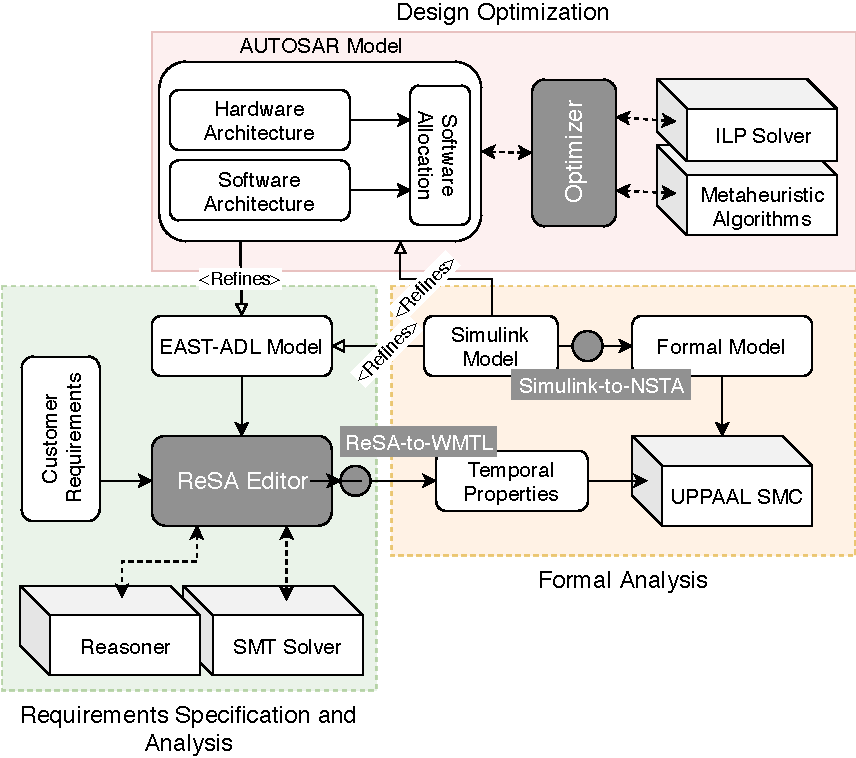
\includegraphics[width=\linewidth]{images/softdevflow}
	\else
	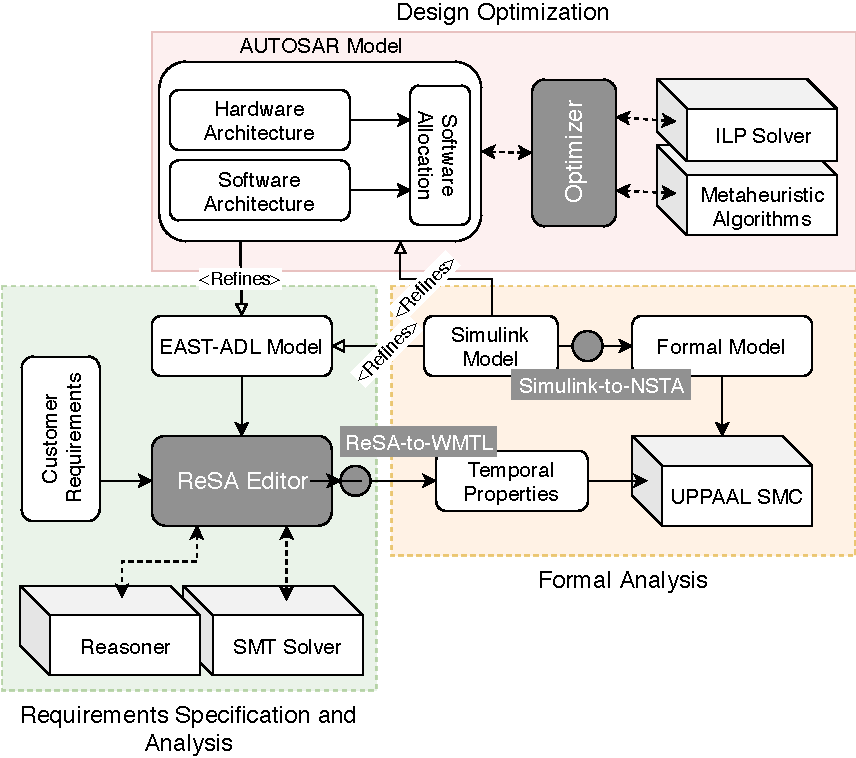
\includegraphics[width=1.0\linewidth]{images/softdevflow.eps}
	\fi
	\caption{Thesis Contributions Workflow.} 
\end{figure}

The rest of the thesis proposal is organized as follows. Section \ref{section:goals} introduces the research goals and the scientific contributions to address the research goals. Section \ref{section:methods} presents the research methods applied to conduct the research especially in the context of academic-industry collaboration. Section \ref{section:outline} shows the proposed outline of the thesis, followed by the presentation of the research progress in Section \ref{section:progress}, including the time plan until the doctoral defense. Section \ref{section:thirdcycle} presents the third-cycle outcomes, adapted from the individual study plan (ISP). Finally, Section \ref{section:related} discusses the related work before concluding the proposal in Section \ref{section:conclusions}.

\section{Thesis Outline Overview}
The thesis is divided into two parts. The first part is a summary of our research. It is organized as follows: in Chapter 2, we give the background information on description logic, Boolean satisfiability problem, Simulink, stochastic timed automata, and meta-heauristic optimization. In Chapter 3, we explain the research problem and outline the research goals. The thesis contributions are discussed in Chapter 4, followed by the related work in Chapter 5. In Chapter 3, we describe the research method applied to conduct the research. Finally, in Chapter 7, we conclude the thesis and outline possible directions for future work.

The second part is a collection of papers included in thethesis, and briefly described listed as follows:
    \chapter{Background}
In this section, we give the necessary background on the different concepts and technologies used in this thesis, which includes requirements boilerplates, logic-based reasoning, Simulink, stochastic timed automata, statistical model checking, integer linear programming and population-based metaheuristics. 

\section{Requirements Boilerplates}
Requirements boilerplates are frequently reoccurring patterns of statements to express software requirements. They have been first introduced to software engineering by Jeremy et al.~\cite{Hull2011RequirementsEngineering} in order to improve requirements specifications by reducing ambiguities and enabling the reuse of specification patterns. A requirement boilerplate consists of static and dynamic syntactic parts. For instance, ``\texttt{if <Condition>, <System> shall be able to <Action> within <Quantity><Unit>.}'' is a conditional boilerplate.  The syntactic elements annotated by pairs of angle brackets are dynamic (or variable), and the rest are static. The engineer has to select the right boilerplates from a repository that suits the target requirements, subsequently filling the dynamic syntactic elements to complete the specifications. 

\section{Logic-based Reasoning}
In this thesis, we express requirements specifications in  Boolean logic and apply \textit{Boolean satisfiability} (SAT) to detect inconsistencies within the specifications. Furthermore, we use \textit{ontology} to represent the specifications, and conduct rigorous analysis via a linguistic approach based on description logic. Consequently, below we briefly overview, SAT, and the notions of ontology and description logic. 

\subsection*{Boolean Satisfiability Problem}
The study of a Boolean formula is generally concerned with the set of truth assignments (assignments of 0 or 1 to each of the variables) that make the formula true. Finding such assignments by answering the simpler question: ``does there exist a truth assignment that satisfies the Boolean formula?'' is called the Boolean satisfiability problem (SAT), which is proven to be NP complete~\cite{devlin2008satisfiability}\cite{Biere2009HandbookSatisfiability}. However, efficient heuristics and approximation algorithms do exist to solve such problems. It is formally defined as follows:
\begin{definition}[SAT Problem]
Given a propositional formula $\phi = (p_1, p_2, p_3, ..., p_n)$ over the logical connectives $\neg,\lor,\land,\rightarrow$, where: $p_1, ..., p_n$ are atomic propositions, the SAT problem equates to checking if there exists an interpretation (or a model) that satisfies $\phi$, that is, a TRUE or FALSE assignment to the variables of $p_1, ..., p_n$, such that $\phi$ evaluates to true, in which case $\phi$ is called satisfiable. In the opposite case, if no such assignment exists, then $\phi$ is unsatisfiable~\cite{devlin2008satisfiability}.  
\end{definition}

SAT problems are usually checked using decision procedures known as SAT solvers. The Z3 tool integrates several background theories (or Satisfiability Module Theories, SMT) and decision procedures based on SAT solvers~\cite{DeMoura2008Z3:Solver}. It is a well known SMT solver and a theorem prover developed by Microsoft Research that has been used in the formal verification and reasoning of software and hardware systems, mainly due to its strong support for integration to verification tools via its well known APIs written, e.g. in Java, Python, C.

The input language of Z3 is an extension of the SMT-LIB2 standard, consisting of commands used to assert logical statements and instruct the solver to do some action, e.g., to check for satisfiability, in which case the command \textit{(check-sat)} is invoked. Z3 returns \textit{sat} if the formulas are satisfiable. If the formulas are not satisfiable, Z3 returns \textit{unsat}, or if it cannot decide the result, it returns \textit{unknown}. In case of unsat, if the unsat-core option is enabled, Z3 can return the subset of unsatisfiable assertions by invoking the \textit{(get-unsat-core)} command.

\subsection*{Ontology and Description Logic}
\textit{Ontology} is a knowledge representation technique frequently used in the artificial intelligence and other domains to facilitate automated decision making. It is defined as ``a formal specification of a shared conceptualization'' according to Borst \cite{Borst1997ConstructionOntologies}. It employs different modeling entities, e.g., concepts, instances, axioms, which are compared to classes, objects, inheritance in Object-Oriented Programming. The ontology is consistent if all axioms and relations (or assertions) hold~\cite{Mankovskii2009OWL:Language}.

\textit{Description logic} (DL)~\cite{Baader2010TheApplications} is a knowledge presentation language, and is the most widely-used language to construct ontologies. It is a fragment of first-order logic with many of the core reasoning problems decidable. For this reason, it has several applications, e.g., in web semantics (e.g., OWL)~\cite{conf/owled/ShearerMH08}, artificial intelligence~\cite{10.1007/978-94-017-9297-4_7}, bioinformatics~\cite{Rector2006}, software engineering, natural language processing. Hence, it is usually backed by solid reasoning services that terminate and deliver results in reasonable time. 

\section{Simulink}
Simulink~\cite{JamesB.Dabney2003MasteringSimulink} is a graphical development environment for the modeling, simulation and analysis of embedded systems, which is widely used in industry to model and inspect the dynamics of systems before implementation. It is robust as it supports multi-domain, continuous, discrete, hybrid systems, also discrete systems that execute with different sampling times (or multi-rate). Figure~\ref{fig_sm_multi-rate} shows a multi-rate subsystem of the Brake-by-Wire Simulink model that models the brake pedal (that is continuous behavior) and global brake functionality (that is, discrete behavior), which execute every 10ms and 20ms.  
\begin{figure}[h]
	\centering
	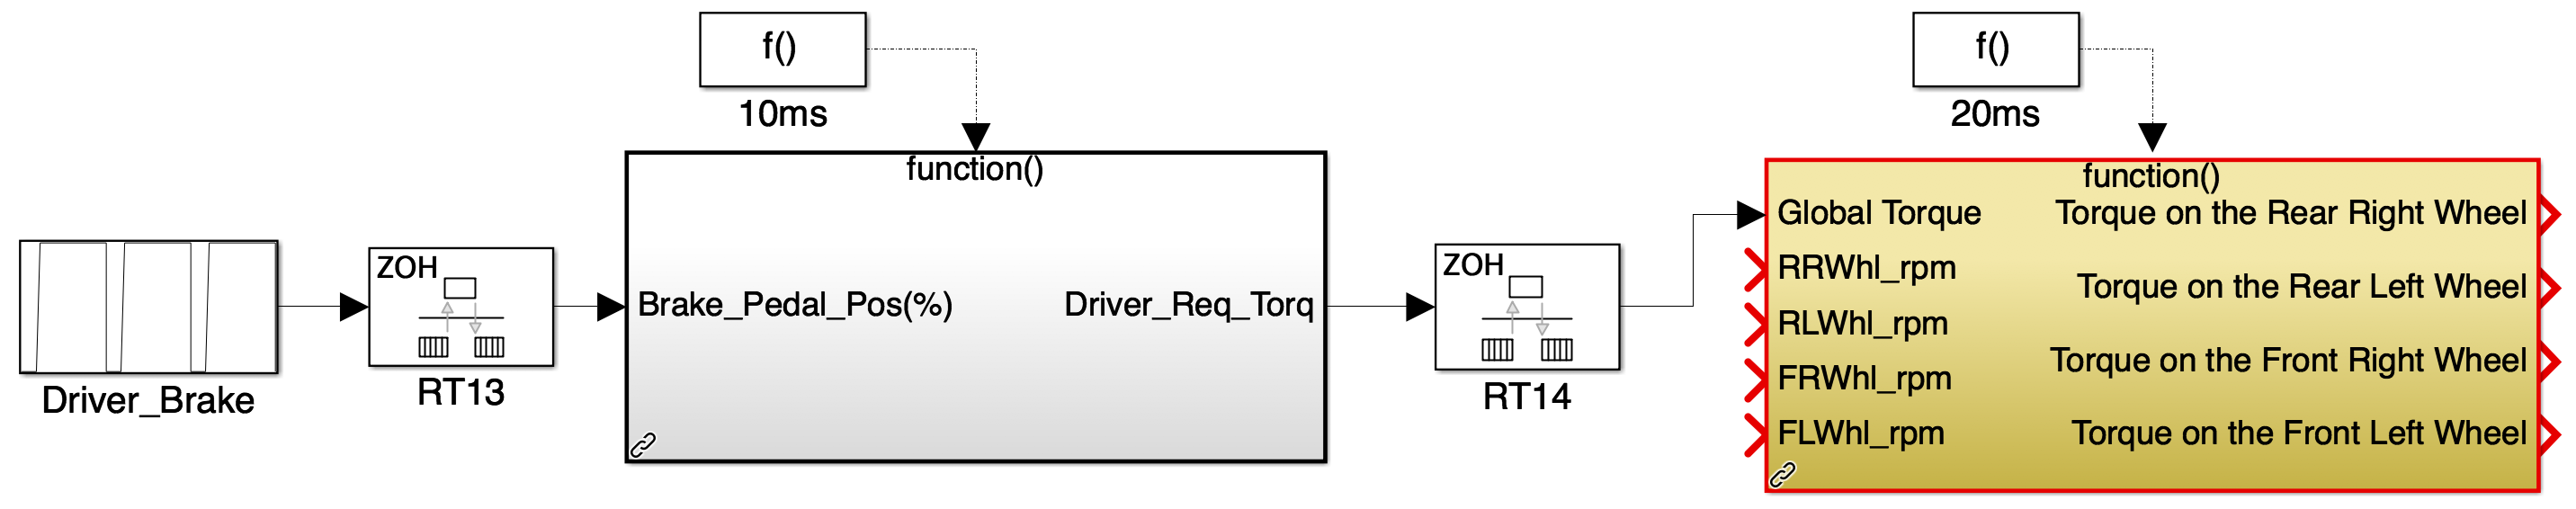
\includegraphics[width=0.9\linewidth]{images/sm}
	\caption{Brake pedal and global brake controller of the Brake-by-Wire model.}
	\label{fig_sm_multi-rate}
\end{figure}

Simulink is frequently used in the development of safety-critical systems, from the automotive, avionics or industrial automation systems domains, being often used to generate code automatically from the models. Therefore, it is crucial that such models are analyzed rigorously. The Simulink~Design~Verifier (SDV)~\cite{MathWokrksSimulinkVerifier} provides a formal verification technique that is based on the exact model checking to exhaustively verify low-level properties such as buffer overflow, division by zero etc. However, the tool's functionality is limited as it lacks support for the analysis of high-level properties, such as invariance, reachability, timing, which is vital to ensure predictability of safety-critical embedded systems. 

\subsection*{Simulink Blocks}
A Simulink model is constructed from communicating function \textit{blocks} (or Simulink blocks). The blocks implement simple to complex functionality and consist of Input and Output ports, which enable communication via connectors. The modeling elements support basic and user-defined datatypes, e.g., integer, floating-point, and simple and complex data structures, namely scalar, vector, matrix.  Simulink blocks are classified into \textit{virtual} (non-computational, e.g., Mux, Demux blocks) and \textit{non-virtual} (computational, e.g., Gain, Integrator) blocks based on their computability. The non-virtual blocks improve the visualization of the model, but unlike the non-virtual blocks, they are not executed, hence do not affect the execution semantics of the model.  The blocks can be composed into groups using Subsystem, Model blocks, to enable hierarchical modeling, which is used to improve the visualization, and to enforce execution order on a group of blocks. The fundamental constructs of the composite blocks are \textit{atomic} blocks, like Gain, Sum blocks.

The non-virtual (computational) atomic blocks can be categorized into \textit{continuous} and \textit{discrete} blocks based on the execution semantics of the blocks.  A discrete block executes periodically with sample time $t_s$, whereas a continuous block executes over infinitesimal sample times. Since the Simulink blocks libraries are not usually sufficient to model practical embedded systems, the framework supports mechanisms to extend functionality, which engineers can exploit to develop complex systems. The mechanisms include S-function, Custom Block and Masking. S-function is a computer language of Simulink blocks which allows advanced implementations of block routines, written in MATLAB, C, C++, or Fortran.


\subsection*{Execution of Simulink Blocks}
During the initial phase of the simulation in the Simulink environment, the model is compiled, thus the order in which the blocks are executed is established in the \textit{sorted order} list (slist). Figure~\ref{fig_sm_exec_order} shows the execution order via the labels in red color, annotated as $s:b$, where $s$ denotes the system/subsystem index and $b$ the block index\footnote{https://se.mathworks.com/help/simulink/ug/controlling-and-displaying-the-sorted-order.html}. Basically, the list is determined according to the data dependency of block outputs on the block inputs ports, that is, if the output depends on the current value of the input, the input port is identified as \textit{direct-feedthrough} port. Thus, to preserve the data dependency in the model, the sort-order rules require that the blocks that derive other blocks with direct-feedthrough ports must come first in the list, e.g., blocks that derive Gain block. However, the blocks with non-direct-feedthrough ports, e.g., the Delay block in Figure~\ref{fig_sm_exec_order}, can execute in any order, considering that the previous rule applies. The execution order is also affected by the user-defined priorities, nevertheless, the priorities do not violate the rules. The sorted order list can be fetched by simulating the model in the debugging mode.
\begin{figure}
	\centering
	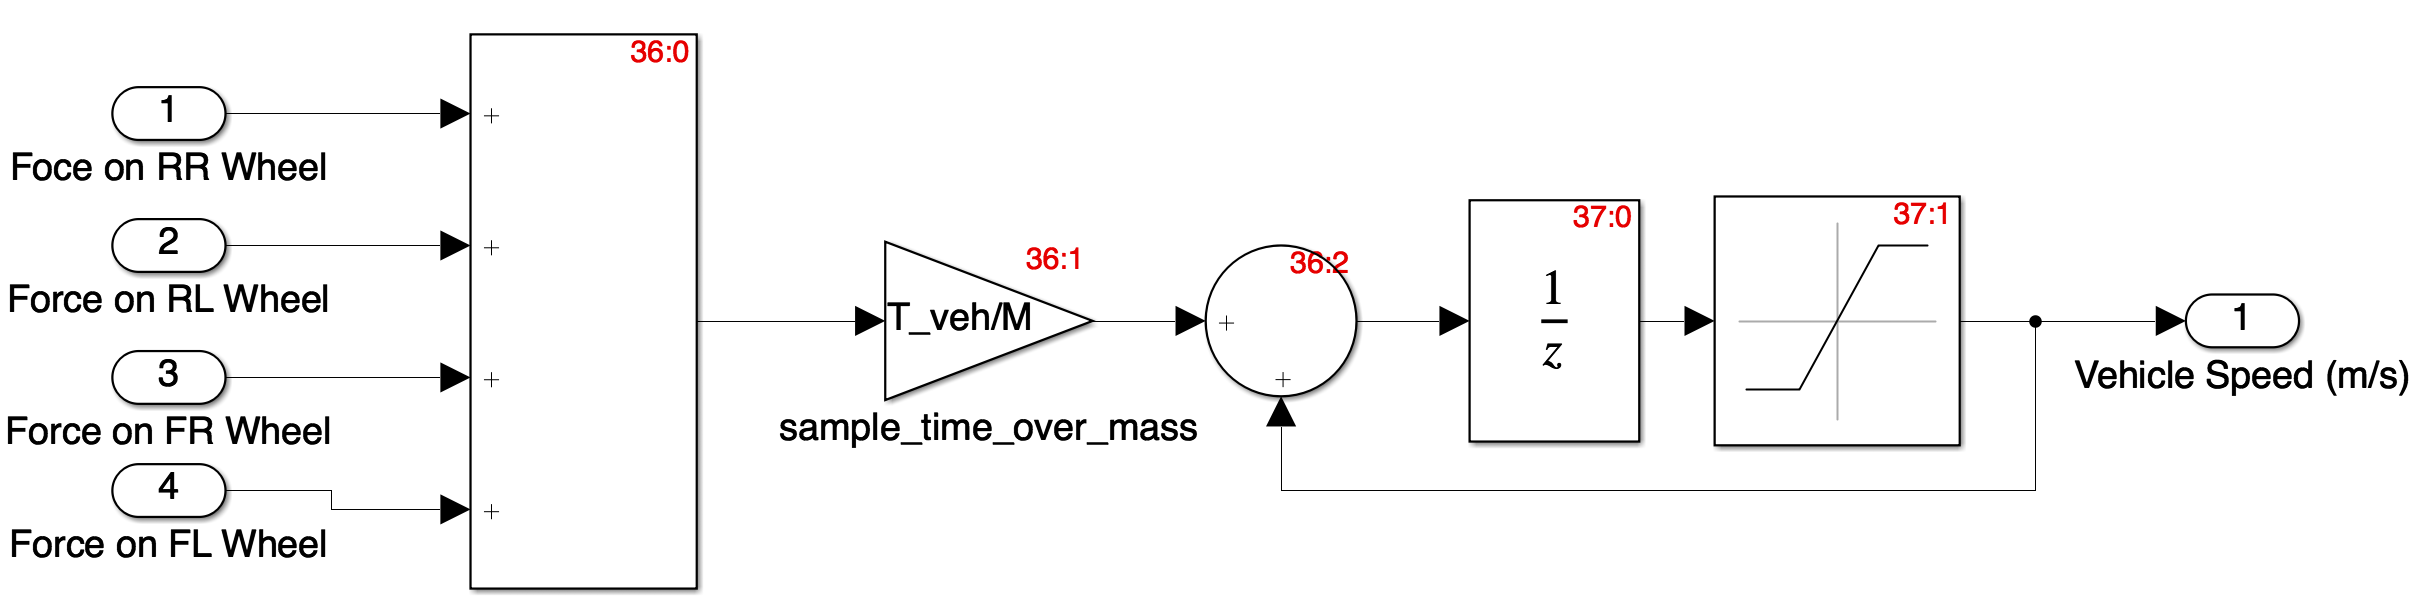
\includegraphics[width=1\linewidth]{images/sm_exec_order}
	\caption{The Brake-by-Wire Subsystem block that computes vehicle speed. The labels in red color denote of the execution order of the blocks.}
	\label{fig_sm_exec_order}
\end{figure}

\section{Stochastic Timed Automata}
The theory of \textit{stochastic timed automata}\cite{David2011StatisticalAutomata} builds upon the timed automata theory and adds probabilistic distributions to support stochastic behavior in modeling and analysis of real-time systems. 

A timed automaton is a finite-state automaton proposed by Alur et al.~\cite{Alur1999TimedAutomata} to model and analyze real-time systems, by extending finite-state automata with real-valued clock variables. A timed automaton (TA) $\mathcal{A}$ is defined as a tuple $\langle L,l_0,X,\Sigma,E,I\rangle$, and its elements are described as follows: $L$ is a set of locations of which $l_0$ is the initial location, $X$ is the set of clocks, $E$ is the set of edges between locations,  $\Sigma$ is a set of action labels, and $I$ is a set of invariants, which are Boolean constraints over $X$ assigned to locations, that is, the automaton can only stay in the location as long as its invariant holds. An edge $(l,g,a,r,l')\in E$ denotes a transition relation from location $l$ to $l'$, with guard $g$, action $a$ and clock resets $r$. The guard is conjunction of clock constraints, and when it holds, the underlying transition corresponding to traversing the edge is fired.


A stochastic timed automaton (STA), as used in \uppaal{} Statistical Model Checker (\uppaalsmc) is defined by the tuple: $STA =\langle\mathcal{A},\mu,\gamma\rangle$, where A is a timed automaton, $\mu$ is the set of all density delay functions, given by either a uniform (for bounded delays via location invariants) or an exponential distribution (for unbounded delays), and $\gamma$ is the set of all output probability functions over the output edges of the automaton. 
\begin{figure}
	\centering
	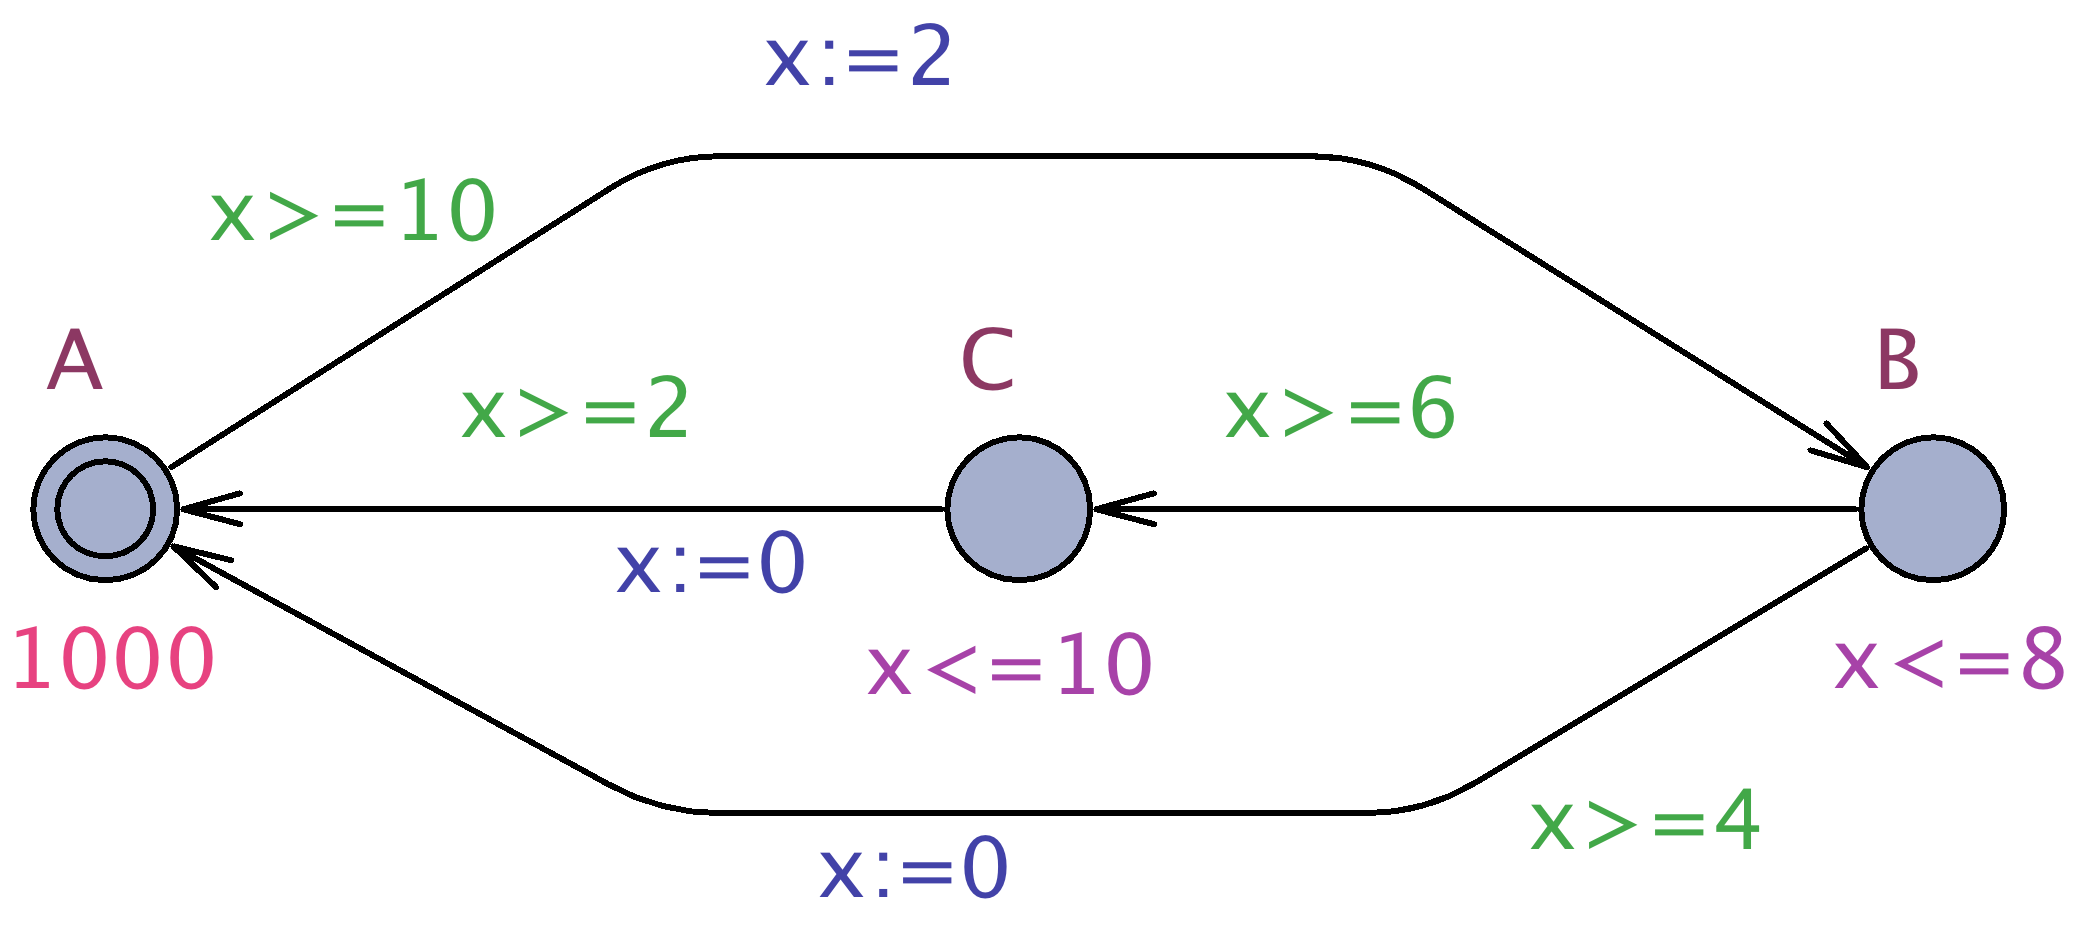
\includegraphics[width=0.6\linewidth]{images/sta_example}
	\caption{STA example.}
	\label{fig_staexample}
\end{figure}

Assume that, $d(l,v)$ is the infimum delay that satisfies the disjunction of guards, and assume that, $D(l,v)$ is the supremum delay before enabling and output. If the delay is bounded, i.e., there exists $D(l,v)$, in location $l$, each delay density function in $l$, $\mu_s$, is assumed to be uniformly distributed in the interval $[d(l,v),D(l,v)]$. However, if the location is time unbounded, the delays are assumed to be exponentially distributed with the rate $R(l)$. For more details on STA, we refer the reader to the literature~\cite{David2011StochasticAutomata}.

\begin{example}[STA Example] Figure~\ref{fig_staexample} is an artificial STA example with three locations A, B and C, where A is the initial location. The guards of the automaton are colored in green (e.g., $x\geq10$ over the edge that connects A and B), the clock resets are colored in blue (e.g., $x=2$ on the same edge), and the location invariants are colored in purple (e.g., $x\leq 10$ on location C). The number in red on location A is the rate of exponential.
The rate of exponential is in fact a user-defined value for the distribution parameter $\lambda$ in the delay function that calculates the probability that the automaton leaves the specified location at each simulation step, as follows:
$Pr(\mbox{leaving location A after } t) = 1 - e^{(-\lambda t)}  = 1000$. Basically, the greater the value of $\lambda$, the higher the probability that the automaton leaves the location.
\end{example}

In the example of Figure~\ref{fig_staexample}, the delays at the location A are exponentially distributed, i.e., with rate 1000, since the location is time unbounded, and delays at B and C are uniformly distributed in the interval $[4,8]$ and $[2,10]$, respectively, since the delays are timed bounded. The output probability at locations A and C is 1 and at location B is 1/2.
%Note: logical path, and probability of taking the path is purely stochastic

\subsection*{Network of Stochastic Timed Automata}
Under the assumption of input-enabledness, disjointness of clock sets and output action sets, a \textit{network of STA} (denoted by NSTA) is parallel composition of $STA_i$~\cite{David2011StochasticAutomata}, that is $(STA_1||STA_2||,...,||STA_n)$, where $n$ is the number of STA in the network. The state of an NSTA is a tuple $\langle s_1,s_2,...,s_n\rangle$, where $s_i = (l_i, v_i)$, where $l_i$ is a location of $STA_i$, and $v_i$ is the valuation of clocks $X_i$. In NSTA, the automata communicate through broadcast channels and globally shared variables. Moreover, the semantics of the NSTA relies on the independent computation of the individual STA (or components), i.e.,  each component automaton, based on the delay density functions and the output probability functions decides repeatedly on which output to generate and at which point in time. In this race, the output will be determined by the component automaton that has chosen to produce the output after the minimum delay~\cite{David2011StatisticalAutomata}.


\section{Statistical Model Checking}
\textit{Statistical model checking}~\cite{Agha2018AChecking} uses a finite set of randomly selected execution traces (or runs) of the state-based system $S$ to check if the traces provide probability evidence for accepting or rejecting the specification (or property) $\varphi$, i.e., $T\in Traces(S)\models \varphi$. It applies statistical techniques such as hypothesis testing and Monte Carlo simulation to compute the probability evidence. Since exhaustive model checking encounters the state-space explosion problem for large models, statistical model checking is a viable alternative to exhaustive verification via probability estimation. 

UPPAAL Statistical Model Checker (\uppaalsmc)~\cite{Bulychev2012UPPAAL-SMC:Automata} is an extension of the model checker \uppaal{} with support for statistical model checking. It admits a system modeled as NSTA, and the properties to checked are specified in probabilistic weighted metric temporal logic (PWMTL)~\cite{David2011StatisticalAutomata}, which is the probabilistic extension of weighted metric temporal logic (WMTL). The properties are of the following form: 
\begin{align}\label{eqn_wmtl}
\varphi::=P(\Diamond_{x\leq T}\phi)\bowtie p | P(\Box_{x\leq T})\bowtie p
\end{align}
where $x$ is a clock, $T\in \mathbb{N}$ is a bound, $\phi$ is a state predicate, $\bowtie \in\{<,\leq,=,>,\geq\}$, and $p \in [0, 1]$.

\uppaalsmc~\cite{David2011TimeSystems}\cite{Bulychev2012UPPAAL-SMC:Automata} can be used to check qualitative properties such as hypothesis testing and probability comparison, as well as quantitative ones via probability estimation. The property $\varphi$ of Equation (\ref{eqn_wmtl}) shows the definition of hypothesis testing. The probability of making hypothesis testing errors is bounded by the strength parameters $\alpha$ and $\beta$, where $\alpha$ is the probability of accepting the null hypothesis while its opposite holds (false negative), and $\beta$ is the probability of accepting the opposite of the null hypothesis while the null hypothesis holds (false positive) and $p$ is the estimated probability of the property holding. Another qualitative property that can be checked using \uppaalsmc{} is the comparison of probabilities.

The probability evaluation is a quantitative method that determines the probability of satisfying a PWMTL property $\varphi$ of an STA. The evaluation is an approximation interval $[p-\mu,p+\mu]$ with a confidence $1-\alpha$, where $\mu$ and $\alpha$ are user configurable parameters. The number of traces is determined automatically by the model checker, based on the parameters. 

\section{Integer linear Programming}
An integer linear programming (ILP)~\cite{Bradley1977AppliedProgramming} is a type of optimization problem that consists of integer decision variables, and the linear objective function and constraints. The binary ILP problem is a special case of ILP where decision variables are binary. It is represented as:
\begin{align}
    \label{eqn_ilp_obj}
	&Maximize\ \sum_{j=1}^{n}{c_jx_j}\\\nonumber
	&\mbox{Subject to:}&\\
	\label{eqn_ilp_cons}
	&\sum_{j=1}^n{a_{ij}x_j}\leq b_i&\mbox{ for all } i=1,...,m\\
	\label{eqn_ilp_bdv}
	&x_j\in\{0,1\} &\mbox{ for all } j=1,...,n
\end{align}
where (\ref{eqn_ilp_obj}) is the objective function with $n$ cost coefficients $c_j:j=1,...,n$, (\ref{eqn_ilp_cons}) are $m$ linear constraints with coefficients $a_j:1,...,m$ and bounds $b_j:1,...,m$, and (\ref{eqn_ilp_bdv}) are binary decision variables with $x_j:1,...,n$.

ILP is used in many control and engineering applications, e.g., fleet and flight routing in transportation, airfoil design in avionics engineering, controller design in industrial automation, automotive, etc., resource allocation. The binary variant is applied in several resource allocation problems, like assignment of operating system tasks to processors. The software allocation, for instance, in component-based development, can be formulated as a binary integer programming problem, where $x_j=1$ denotes the fact that a component is mapped to the $j^{th}$ processor and $x_j=0$ denotes the fact that a component is not mapped to the $j^{th}$ processor.

ILP problems are frequently solved via exact algorithms, e.g., branch and bound, but can also be dealt with heuristics, e.g., using simulated annealing, hill climbing. In this work, we use the CPLEX solver~\footnote{https://www.ibm.com/analytics/cplex-optimizer} form IBM to the software allocation optimization.'

\section{Population-based Metaheuristics}
The ILP approach and for that matter exact methods do not scale well on complex optimization problems, or else their application is usually prohibitively expensive when applied on large-scale problems, i.e., with many decision variables. In contrast, metaheuristics~\cite{2006HandbookMetaheuristics}\cite{Gonzalez2007HandbookMetaheuristics}, which is a type of heuristics with search strategy, is more efficient computation-wise, albeit less optimal. The population-based metaheuristics is a class of meta-heuristic algorithms which uses a set of individuals (or population) to guide the search strategy and determine the global optima of the problem. The most common population-based algorithms consist of evolutionary algorithms, differential evolution~\cite{Storn1997DifferentialSpaces}\cite{Das2016RecentSurvey}, particle swarm optimization~\cite{Poli2008AnApplications}\cite{Mirjalili2019ParticleOptimisation}.

In this thesis work, for the efficient software allocation, we apply the differential evolution, particle swarm optimization (PSO) and the latter's hybrid with local search algorithms such as hill climbing and stochastic hill climbing to find the best (or near optimal) solution. In the case of differential evolution, special evolutionary operators, such as mutation, crossover and selection, are employed to update the population, thus traverse across the search space to reach at the global near-optima. The technique is briefly described as follows. A mutant agent (or individual), i.e., the offspring $\textbf{v}$, is generated for every agent from three other agents in each iteration according to (\ref{eqn_de_mutation}), subsequently combined using the crossover operator (\ref{eqn_de_crossover}). If the offspring $\textbf{u}$ is more fit than the agent $\textbf{x}$, i.e., closer to the best solution, it replaces the agent otherwise is discarded as shown in the selection strategy (\ref{eqn_de_selection}).
\begin{align}
\label{eqn_de_mutation}
\textbf{v} & \leftarrow   \textbf{a} + F\circ(\textbf{b}-\textbf{c})\\
\label{eqn_de_crossover}
\textbf{u}&\leftarrow crossOver(\textbf{v},\textbf{x},CF,F)\\
\label{eqn_de_selection}
\textbf{x} &\leftarrow 
\begin{cases}
	\textbf{u} & \mbox{if } f(\textbf{u}) < f(\textbf{x})\mbox{ functions}\\
	\textbf{x} & \mbox{otherwise }
\end{cases}
\end{align}
where $F\in[0,2]$ is known as differential weight and controls the diversity of the mutant, and $CF\in[0,1]$ is known as the crossover probability and controls the degree of crossover between the agent and the mutant.

Similarly, the particle-swarm optimization employs individuals (or particles in this case). The particles unlike in the differential evolution are memory-based, i.e., they record their best position so far $\textbf{p}_{bst}$, and the algorithm remembers the best position of the population $\textbf{z}$. The motion of each particle is guided by its velocity (\ref{eqn_pso_velocity}) and attractions towards its best position $\textbf{p}_{bst}-\textbf{p}$ and towards the best position of the population $\textbf{z}-\textbf{p}$ (\ref{eqn_pso_position}), where $\textbf{p}$ is an n-dimensional matrix which represents the current position of a particle.
\begin{align}
\label{eqn_pso_velocity}
\textbf{v} &\leftarrow  \omega\textbf{v} + c_1Rand()\circ(\textbf{p}_{bst}-\textbf{p}) + c_2Rand()\circ(\textbf{z}-\textbf{p})\\
\label{eqn_pso_position}
\textbf{p} &\leftarrow \textbf{p} + \textbf{v},
\end{align}
where $\omega$ is the weight of the velocity, also known as \textit{inertia coefficient} and controls the convergence of the algorithm. The $c_1, c_2$ constants are acceleration coefficients and control the weight of attraction towards the cognitive and social components, respectively. $Rand()\in U(0,1)$ is a random function along the acceleration coefficients, which is element-wise multiplied with the components to improve diversity of the search by introducing stochastic behavior
    \chapter{Problem Formulation}
The automotive electrical/electronic system executes complex safety-critical software, e.g., x-by-wire software, engine control, traction control, etc. Over the last decades, the complexity of the safety-critical software has been on the rise which is evident on the modern cars, which implement many and complex automotive functions, and also on the emergence of the electrical and autonomous vehicles. Thus, the thesis is motivated by the need for advanced (or rigorous) methods to the requirements specification, modeling and analysis of the complex safety-critical automotive software, and their seamless integration into the existing methods and tools of the automotive systems development at VGTT and Scania. Furthermore, the thesis is motivated by the need for efficient mapping of safety-critical software to hardware in the distributed computing to facilitate software extensibiliy and support the increasing functionality of the automotive systems. 

Thus, the \textit{overall goal} of the thesis is to:
\begin{mybox}[attach title to upper={\ ---\ }]{Overall Goal}
	Provide assurance of safety-critical functionality, at the various levels of abstraction, via formal analysis, and optimization of critical system resources.
\end{mybox}

The overall goal is refined via \textit{research goals}, which state the needs or concerns that the thesis should address and are formulated as follows:

\section{Research Goals}\label{research_challenges}
Many safety-critical automotive systems are developed according to the ISO 26262 standard, which recommends highly the use of semi-formal languages to specify safety-critical requirements to improve quality of the specifications, e.g., by reducing ambiguity and improving comprehensibility. In the context of textual representations, the semi-formal specification methods are constrained natural languages, such as templates (e.g., requirements boilerplates~\cite{Farfeleder2011DODT:Development}\cite{Mahmud2015ReSA:Systems}), controlled natural languages~\cite{Kuhn2014ALanguages}(e.g., Attempto~\cite{attempto96}).

The template-based methods inherently lack meta-model (or grammar), therefore is difficult to add new templates effectively, moreover, template selection is usually cumbersome. The existing controlled natural languages lack effective support of specifying embedded systems requirements.

Thus, the first research goal is to:
\setcounter{rgcounter}{1}
\begin{researchgoal}
Reduce ambiguity and improve the comprehensibility of natural-language requirements using domain-specific knowledge of embedded systems.
\end{researchgoal}

One of the mechanisms to improve natural language specifications is by constraining the language, including its syntax, semantics and the lexicon \cite{Kuhn2014ALanguages}. The design of a constrained natural language for the specification of requirements is not trivial. By constraining the language, its expressiveness and intuitiveness can be impaired~\cite{ieereqspecstandard}\cite{Myachykov2013SyntacticRussian}, therefore, appropriate trade-offs should be made during the design in order to have a robust and effective specification language.

Besides improving quality of individual requirements, the latter should be analyzed in ensemble in order to detect errors that span multiple specifications, e.g., logical contradictions. However, natural language lacks formal (or precise and unambiguous) semantics, therefore is difficult to rigorously analyze (or reason) natural-language requirements specifications. There are several methods to natural language semantics, of which the use of \textit{logic} is common~\cite{Clark2010TheProcessing}.

Thus, the second research goal is to:
\begin{researchgoal}
Facilitate formal analysis of the requirements specifications through transformation to Boolean and description logics.
\end{researchgoal}

Natural language specifications are constructed from syntactic units, such as words, phrases, clauses, statements, etc. Consequently, rigorous analysis of the specifications involve parsing and interpreting the syntactic units, which is a complex problem in computational linguistics~\cite{Clark2010TheProcessing}. The depth of the interpretation (or semantics) greatly affects the applicability of the methods, e.g., the propositional logic representation of the specifications is simple and the analysis scales well, however, it is shallow as it abstracts away the details. On the other hand, the first-order-logic representations are more rigor, thus enable thorough analysis but are less tractable. Therefore, appropriate interpretation of the natural language specifications is crucial.

The software designs and software-design units (or behavioral models) should conform to the requirements specifications. We consider the software-design units are modeled in Simulink, which is the most widely used model-based development environment in industry to model and simulate the behavior of multi-domain, discrete, continuous embedded systems. Simulink also enables the generation of code from discrete Simulink models which directly execute on specific platforms, thus is crucial to conduct rigorous analysis of the Simulink models to reduce errors introduced in the generated code.

The de~facto Simulink analysis techniques, e.g., by type checking, simulation, and formal verification via the Simulink Design Verifier (SDV\footnote{https://se.mathworks.com/products/sldesignverifier.html}) are not sufficient to address the full correctness of safety-critical real-time Simulink models. SDV lacks support for checking temporal correctness as specified in timed properties, e.g., in TCTL, and also lacks support for verifying continuous models and suffers from scalability due to its reliance on the exact model-checking~\cite{Leitner2008SimulinkStudy}. In contrast to the exact model checking, the statistical model-checking verifies properties over sufficiently collected traces of system simulations via statistical methods. It scales better over the trade-off for exhaustiveness. 

Thus, the third research goal of the thesis is to:
\begin{researchgoal}
Enable formal analysis of large-scale, multi-rate and hybrid Simulink models using statistical model-checking.
\end{researchgoal}

Simulink consists of connected and hierarchical Simulink blocks, which encode mathematical functions~\cite{JamesB.Dabney2003MasteringSimulink}. For industrial systems, the number of blocks in a Simulink model can be in the order of thousands, and the blocks can be triggered with different sampling frequencies for discrete blocks and without any sampling frequency 
for continuous blocks. Therefore, typical industrial Simulink models are usually complex and comprise mixed signals, multiple rates, discrete and continues Simulink blocks, making the model checking challenging.

In the distributed computing, the automotive software is allocated on multiple computing units (or ECU), consequently is exposed to higher permanent and transient faults, hence necessitates to maximize the reliability of the safety-critical software system. Fault tolerance using redundancy is the most widely approach to improve reliability such as by replicating software functionality on multiple ECU, however, it requires additional critical system resources such as power sources. In this regard, the software-to-hardware allocation plays a crucial role to minimize the power consumption of fault-tolerant distributed safety-critical software while satisfying the timing and reliability constraints of the safety-critical software.

Thus, the fourth research goal is to
\begin{researchgoal}
 Minimize the power consumption of distributed safety-critical software while satisfying the timing and reliability constraints during the software allocation.
\end{researchgoal}

The software allocation model is not trivial as we consider exact method of schedulability analysis and reliability calculations, which makes the optimization complex. We assume a sufficient and necessary scheduling test based on the worst-case response time analysis~\cite{Baruah2011Response-timeSystems}\cite{Davis2007ControllerRevised}, moreover end-to-end delay analysis based on the age delay semantics~\cite{mubeen2013support}, which is practical but computationally expensive. For the reliability analysis, we apply an exact method of calculation based on the state enumeration, in contrast to the series-parallel method, which is trivial and computationally less expensive. As a result, we consider an exact optimization method using ILP for relatively small and metaheuristics for relatively large software allocation problems.

In order to show the validity of our proposed solutions, a working prototype should be developed and should also be evaluated on industrial uses cases. The validation should consider scalability and engineer-friendliness of methods and tools besides effectiveness. 

Thus, the last research goal is to:
\begin{researchgoal}
 Provide automated and engineering-friendly support for the requirements specification, software allocation of embedded  and formal analysis of Simulink models.
\end{researchgoal}

Seamless integration of our proposed methods and tools into the existing development process require close cooperation between the domain experts and the practitioners. The role of the domain experts should be to simplify usage of the tools, e.g., by rendering their interface to existing once, etc., and the practitioners should cooperate with materials that assist the validation of the proposed solutions. The cooperation is not trivial considering the challenge of formal methods, and companies culture for being restrictive.

    \chapter{Thesis Contributions}
The overreaching contribution of the thesis is a design approach targeting safety-critical embedded software, which employs formal methods at various stages of software development, such as requirements specification and software design, and a power-efficient allocation of software to distributed hardware. Our approach meets the research goals defined in Section~\ref{ch_problem_formulation}, via the following contributions: a requirements specification language tailored to embedded systems~\cite{Mahmud2015ReSA:Systems}, formal analysis of the specifications~\cite{resatool}\cite{Mahmud2017SpecificationLogic} via logic-based methods, formal analysis of large-scale Simulink models via statistical model checking~\cite{Filipovikj2018SimppaalModels}, and efficient mapping of software to hardware in the context of distributed architectures, via integer linear programming and hybrid particle swarm optimization~\cite{Mahmud5222}\cite{Mahmud2019OptimizedConstraints}. 

\section{Design Workflow: Contributions Overview}
In Figure~\ref{fig_workflow}, we illustrate the workflow of an embedded software development that make of use our contributions. The workflow is contextualized in the automotive systems development where Simulink\footnote{Matlab Simulink - \url{https://se.mathworks.com/products/simulink.html?requestedDomain=}}, as well as architectural languages such as \eastadl\footnote{EAST-ADL - \url{https://www.east-adl.info/}} and \autosar\footnote{AUTOSAR - \url{https://www.autosar.org/}} are used.
\begin{figure}
	\centering
	\ifpdf
	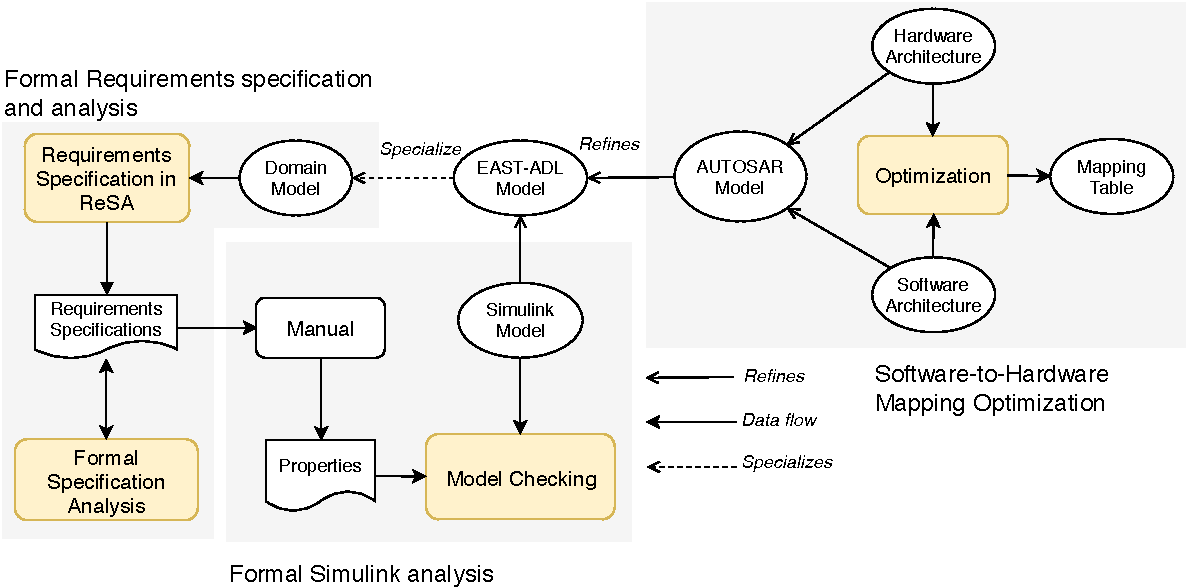
\includegraphics[width=\linewidth]{images/workflow}
	\else
	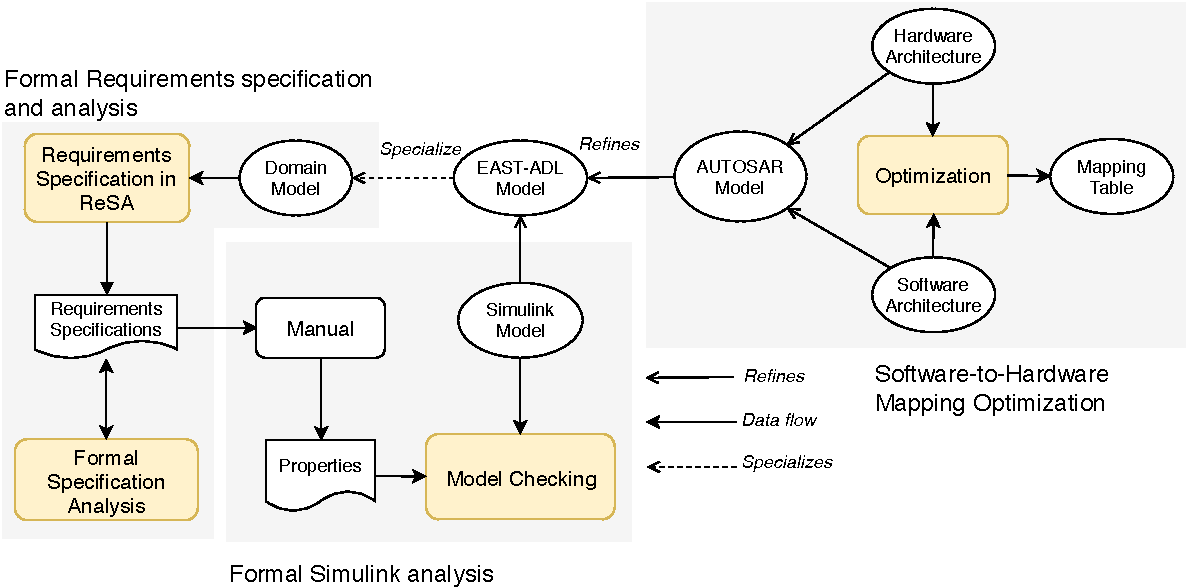
\includegraphics[width=.8\linewidth]{images/workflow.eps}
	\fi
	\caption{Thesis contributions workflow.} 
	\label{fig_workflow}
\end{figure}

Initially the textual requirements are specified in our domain-specific language \resa, which is a constrained natural language tailored to embedded systems. The \resa{} editor supports content completion as it is connected to a system model, which contains instantiations of words/phrases. If the \resa{} editor is required to be domain-specific, e.g., to the automotive domain that employs \eastadl, the system model is specialized to the latter model, thus enabling requirements specifications by accessing \eastadl{} model elements from the editor. To check the consistency, the \resa{} specifications are translated into Boolean and description logic, respectively, and subsequently analyzed via SAT solver and inference engine (or reasoner), respectively.

After the quality of the specifications is checked and improved if needed, that is made unambiguous, comprehensible, consistent, they can be used in the verification of behavioral software designs. In this thesis, we consider that the software design is created with Simulink, which is one of the most popular integrated environments for modeling, simulation and analysis of embedded system functions. In order to analyze a Simulink model rigorously, we transform it automatically into a formal model, specifically a network of stochastic timed automata. Subsequently, the latter is analyzed via statistical model checking against properties initially expressed in \resa, but manually translated into the query (properties) language of the model checker, that is probabilistic weighed-metric temporal logic (PWMTL).

At the architectural level, the Simulink model is represented by \eastadl{}, and at the implementation level by an \autosar{}, which consists of software components that communicate through a virtual function bus (VFB).  Note that, the refinement from the \autosar{} model to the Simulink model is manual, which is the normal practice, however, the Simulink model composition (or structure) is automatically generated. The software architecture complements the Simulink model with computation resource specifications, that is via runnables, which are schedulable pieces of code (or objects) by the \autosar{} OS. Moreover, AUTOSAR also complements Simulink models with resource specifications, such as power specification, interface specification of the underlaying hardware, etc. In this regard, we propose exact and heuristic software-to-hardware optimization techniques that incorporate the timing and reliability of software applications as constraints, and optimize the power consumption of the software.

The thesis contributions are summarized in the next sections. 
\section[RC1: {\sffamily \resa{}} -- \textbf{Re}quirements \textbf{S}pecification L\textbf{A}nguage]{RC1: \\{\sffamily ReSA} -- \textbf{Re}quirements \textbf{S}pecification L\textbf{A}nguage}\label{rc_resa}
We propose a domain-specific and constrained natural language, both at the syntax and semantics level, which is designed to improve comprehensibility and reduce ambiguity of embedded systems requirement specifications. The language employs concepts from the embedded systems domain, e.g., \textit{System}, \textit{Parameter}, \textit{Device}, \textit{State}, \textit{Mode}, \textit{Entity}, to typeset domain-specific words/phrases. Besides grammatical rules (or syntax), semantic relations between the concepts limit the possible construction of the specifications. For instance, the sentence``The ASL shall limit the driver.'' is a grammatically-correct specification, but semantically it makes no sense. To solve this problem, the \resa{} type system imposes a type constraint on the relation between instances ``The ASL''\textit{:system} and ``the driver''\textit{:user}.

\subsection*{Syntax}
The language design is modular, in the sense that it uses sentence categories, e.g., \textit{Simple}, \textit{Compound}, to structure the specifications, thus improve comprehensibility and reduce ambiguity. It also allows complex specifications by inductively applying the grammar rules of the language. The following context-free grammar is a snippet of the \resa{} language. 
\begin{bnf*}
	\bnfprod{specification}
	{\bnfpn{simple} \bnfor \bnfpn{complex}\bnfor\bnfpn{nested-complex} ...}\\
	\bnfprod{simple}
	{\bnfpn{mainClause} .} \\%\bnftd
		\bnfprod{complex}
	{\bnfpn{subClause}, \bnfpn{mainClause}.} \\%\bnftd
	\bnfprod{mainClause}
	{\bnfpn{primitiveClause}\bnfor ...} \\%\bnftd
		\bnfprod{primitiveClause}
	{\bnfpn{sub} \bnfpn{verb} \bnfpn{obj}\bnfor...} \\%\bnftd
	\vdots
\end{bnf*}
For the detailed grammar specification of the language, the reader is invited to refer to Paper~A~\cite{Mahmud2015ReSA:Systems} and its documentation
\footnote{ReSA documentation:  \url{https://bitbucket.org/nasmdh/resa/src/master/} }
\begin{example}[Adjustable Speed Limiter (ASL) Requirements]\label{ex_resa_example}
	We here give an example of selected requirements of the ASL system, which is a speed control system found in Volvo trucks. It controls the vehicle speed to not exceed a certain speed, which is set by the driver or legal authorities. It consists around 300 fuctional and extra-functional requirements. Just to demo the usage of the language, we specify only four of ASL equirements.
\begin{elaboration}{0.95}
	\small
		\begin{tabular}{lp{.9\textwidth}}
			R1 & ASL:system shall send "the driver"\textit{:user} notification:status every 200ms. \\
			R2 &\begin{tabular}[t]{@{}l@{}}if ``driver:user'' selects ``ASL speed control''\textit{:mode} and\\
				\hspace{0.5cm}(vehicle is in ``pre-running'' mode or
				vehicle is in ``running'' mode)\\ then\\
				\hspace{0.5cm}ASL:system shall be enabled within 200ms and\\
				\hspace{0.5cm}``ASL enabled''\textit{:status} shall be presented to ``the driver''\textit{:user} \\ endif\end{tabular} \\
			R3 & After ASL:system is enabled, if IncButton\textit{:inDevice} is pressed, ASL:system shall be activated.\\
			R4 &if driver selects ``ASL speed control''\textit{:mode}
			then 
			ASL\textit{:system} shall be disabled.
		\end{tabular}
\end{elaboration}
\end{example}

\subsection*{Tool Support and Validation on Adjustable Speed Limiter}
The \resa{} language is implemented~\cite{resatool} in the Xtext framework\footnote{\url{Xtext: https://www.eclipse.org/Xtext/}}, which is an Eclipse-based integrated development environment for the development of domain-specific and general-purpose languages. The \resa{} editor, which is shown in Figure~\ref{fig_resagui}, supports content completion, errors/warring messages and boilerplate management. The editor is integrated in \eatop, meaning that the editor can be triggered from within the IDE, moreover, the content-completion feature displays contents of the \eastadl{} model elements, hence enabling the consistent use of vocabularies during specification. The \resa{} tool as a standalone, and as a plugin for \eatop{}, can be downloaded from the URL {\small \url{https://bitbucket.org/dashboard/overview}}. 
\begin{figure}[h]
	\centering
	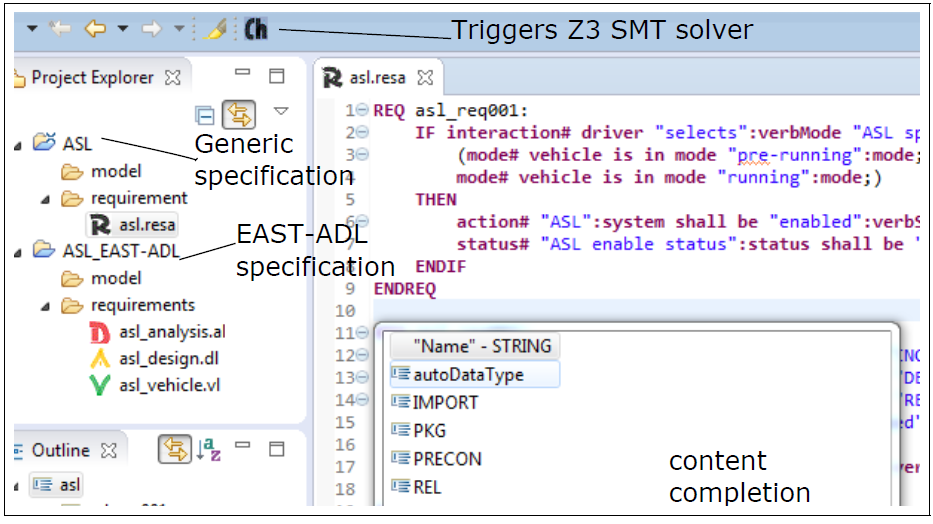
\includegraphics[width=1\linewidth]{images/resagui}
	\caption{The \resa{} graphical user interface (GUI).}
	\label{fig_resagui}
\end{figure}

The language as well as its tool support is validated on the 300 ASL requirements, which are initially expressed in natural language. The requirements distribution is as shown in Figure~\ref{fig_ASLreqs}, in terms of types of requirements. The requirements are rewritten in \resa, and Figure~\ref{fig_ASLreqsresult} shows the sentence categories (or boilerplates) employed to specify the requirements. In general, the language is expressive, though it is constrained, and is extensible with constructs that improve its expressiveness.
 \begin{figure}[h] 
 	\centering
 	\subfloat[Types of ASL Requirements.\label{fig_ASLreqs}]{% 
 		\centering
 		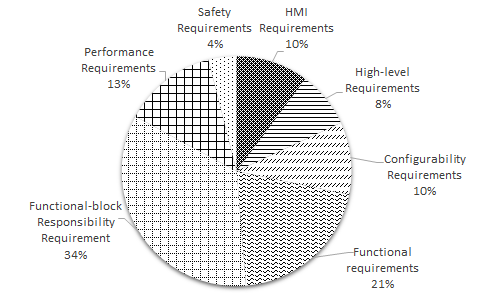
\includegraphics[width=0.45\textwidth]{images/aslreq}
 	} \hfill
 	\subfloat[Distribution of ASL boilerplate types.\label{fig_ASLreqsresult}]{% 
 		\centering
 		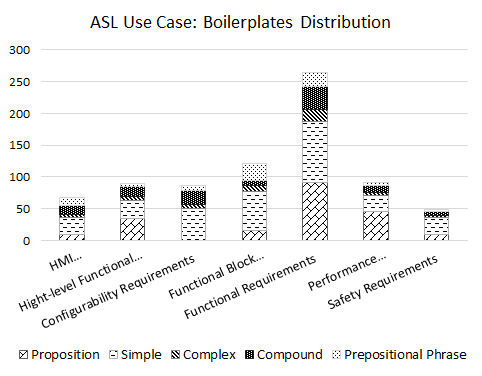
\includegraphics[width=0.45\textwidth]{images/aslbp} 
 	} 
 	\caption{Specifying ASL requirements in \resa.} \label{fig_resa_asl}
 \end{figure}
\section[RC2: Consistency~Checking of {\sffamily ReSA}~Specifications]{RC2: \\Consistency Checking of {\sffamily ReSA} Specifications}\label{rc_resaanalysis}
The editor shows syntax and typing warning and error messages. However, such static analysis is rudimentary and is per specification. In this contribution, we propose two methods of consistency analysis: \textit{SAT-based} analysis and \textit{ontology-based} analysis, which analyze over multiple specifications.

\subsection*{SAT-based Analysis}
Boolean satisfiability (also known as SAT) can informally be defined as the problem of finding truth values (or assignments of Boolean variables) such that a Boolean formula holds. It is NP-complete, however, there exist efficient heuristic algorithms that solve SAT problems of large size, e.g. with thousands of Boolean variables. Therefore, we first transform the \resa{} specifications into Boolean expressions~\cite{resatool}, then we formulate the problem of finding inconsistencies of the Boolean expressions, in terms of SAT as follows:
\begin{definition}[Inconsistency of Specifications]
	Let $\Phi = \{\Phi_1, \Phi_2,\dots,\Phi_n\}$ be the \resa{} specifications and after translating its constituents into Boolean expressions,  $\phi_i, i \in [0,..,n]$. Consequently, $\phi_1, \phi_2,...,\phi_n$ are Boolean formulas, each denoting a requirement respectively. We say that the set of Boolean formulas $\phi$ is \textit{inconsistent} if the expression $\phi_1 \land \phi_2 \land\dots\land \phi_n \Rightarrow false$ holds, that is, there exists at least one expression that cannot be satisfied:  $\exists i. \phi_i |= false$. 
\end{definition}
\begin{example}
Assume that we want to check the consistency of the requirements that are specified in Example~\ref{ex_resa_example}. Figure~\ref{fig_z3} shows the translation of the specifications into Boolean expressions (in Z3  SMT-LIB format). Each expression is asserted before the Z3 solver is called using the command $(check-sat)$. Some clauses are resolved for negation and opposite words, e.g., the fact that ``enabled'' is opposite of ``disabled'' implies $p_5=p_7\neq p_{11}$. The solver returned ``\textit{unsat (R2 R4 R1\_Assertion)}'',  which means, the expressions are inconsistent and indicates the specifications that are responsible for the inconsistency (or unsat-core).
\end{example}
\begin{figure}[h]
	\centering
	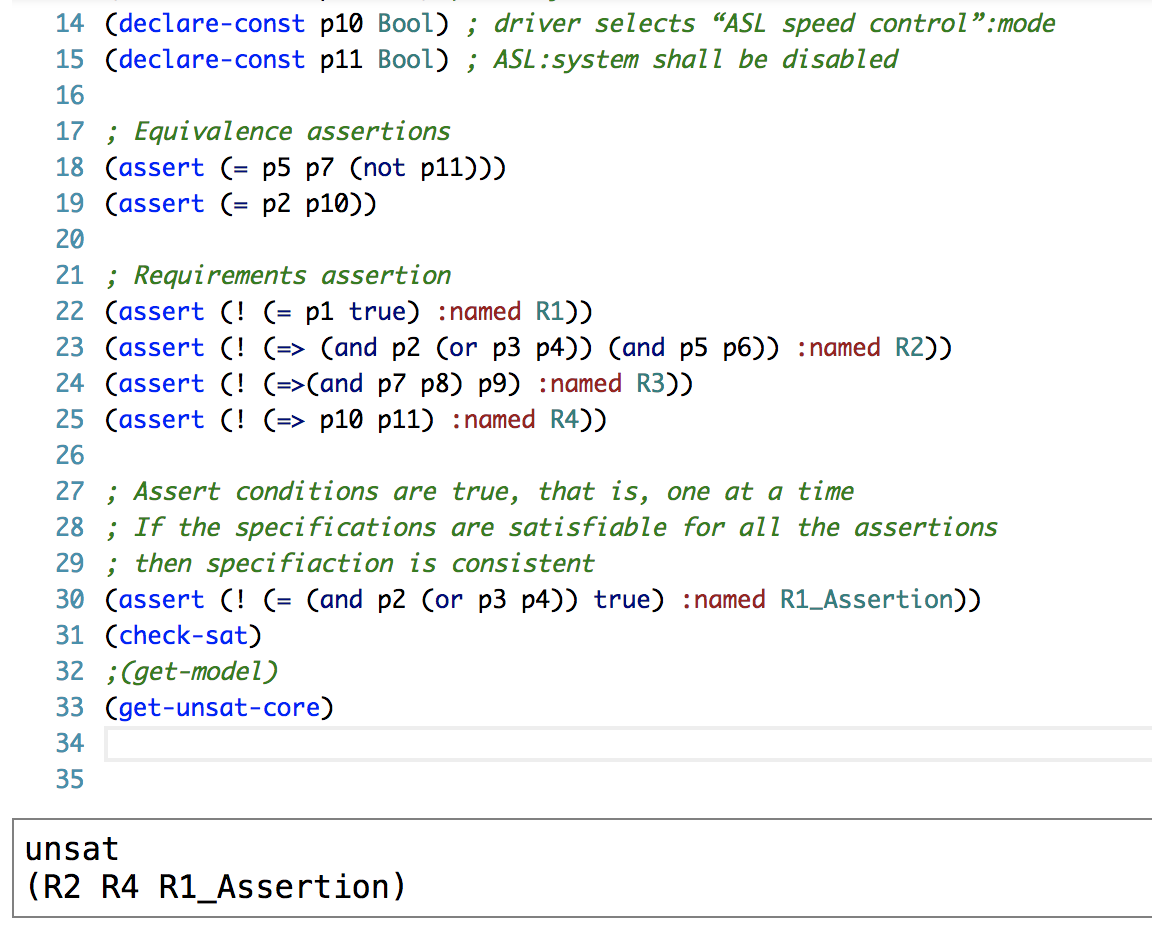
\includegraphics[width=0.7\linewidth]{images/z3}
	\caption{The \resa{} specifications R1 - R4 encoded as Z3 format, and the unsat-core feedback from the Z3 solver, to localize the source of the inconsistency.}
	\label{fig_z3}
\end{figure}

The SAT-based analysis, although easy and scalable, does not allow rigorous analysis. This is due to the fact that the Boolean (or propositional) variables abstract away details of the clauses in the specifications. %The ontology-based approach solves this problem with trade off over scalability.

\subsection*{Ontology-based Analysis}
\textit{Ontology} as a knowledge representation technique can be used to capture the intricate relations of words/phrases of specifications, for instance, synonyms, antonyms, generalization. Moreover, it can be used to capture the syntax of the specifications as well, essentially modeling the \resa{} specification as a concrete requirements specification ontology. 

Besides the challenge of constructing the ontology, accurate representation of the specifications is crucial to a certain degree for the ontology to be useful, that is, the specifications should be interpreted linguistically. In this research, we propose the \textit{event-based} semantics approach~\cite{Mahmud2017SpecificationLogic} to construct the meaning of each specification compositionally from its constituents (or grammar units). The event-based semantics, which is based on the first-order logic, uses an existentially-quantified events to relate words/phrases (or arguments of predicate) , clauses, adjuncts of a sentence~\cite{Mahmud2017SpecificationLogic}. To help intuition, let us assume the following example: the clause ``ASL:system shall limit ``vehicle speed'':parameter'' is represented as $\exists e$[limiting($e$) \& Agent(ASL) \& Recipient(vehicle speed)], where Agent and Recipient are known as \textit{thematic} roles, which define the semantic roles of the arguments in the clause.  Since the requirement specifications entail technical words/phrase, the thematic roles of these arguments are not obvious, so we extended the thematic roles into the \resa{} concepts, in this way, the interpretation of the clauses becomes domain-specific, for example, classifying instances of \textit{System} or \textit{User} as \textit{Agent}, and  instances of \textit{Parameter} as \textit{Recipient}.  

Following the event-based semantics, the \resa{} specifications are translated into description logic as ontology. Once the ontology is constructed considering the event-based semantics, thematic roles, lexical relation, we check its consistency via an inference engine (or reasoner), which is a software program that applies logical rules on a logical system, such as the ontology, to obtain new information.
\begin{definition}[Inconsistency of Specifications]
	The requirements specification ontology is inconsistent if there does not exist an interpretation (or a model) $M$ that satisfies the terminological assertions $T$ and the concrete assertions $A$, that is, $M \not\models ax$, where: $ax \in T \cup A$, where $T$ is a set of terminological assertions and $A$  a set of facts (or concrete assertions).
\end{definition}

\section[RC3: Statistical~Model~Checking~of~Simulink Models]{RC3: \\Statistical~Model~Checking~of~Simulink Models}\label{rc_sim}
Several research endeavors do exist on the topic of formally analyzing Simulink models. Some of them are using theorem proving, others exact model checking and others statistical model checking. Many of the proposed solutions are  limited either due to frequent user involvement or scalability issues. In this thesis, we propose a scalable formal analysis of large-scale Simulink models via statistical model checking. The Simulink models can be discrete, continuous or hybrid, moreover, they can consist of atomic and composite Simulink blocks that are scattered on multiple files, which is a practical scenario. Essentially, we consider typical industrial Simulink models, e.g., the Brake-by-Wire and Adjustable Speed Limiter Simulink models from VGTT~\cite{Filipovikj2018SimppaalModels}.

To enable statistical model checking of Simulink models, we first define the syntax and semantics of blocks and their composition, in terms of timed transition systems. After that, we transform the Simulink blocks of a model, after flattening, in networks of stochastic timed automata that can be model checked statistically with \uppaalsmc.  Our approach has the following important characteristics: (i) the transformation employs continuous and discrete transformation patterns, which are generic and reusable, thus can be applied to any Simulink blocks; (ii) the transformation preserves the execution order of Simulink blocks; (iii) it is robust, meaning that, it handles various models such as continuous, discrete, hybrid, and models that contain blocks with with different sampling rates, also known as multi-rate blocks.

\subsection*{Transformation Patterns} 
The continuous-time and discrete-time stochastic timed automata (STA), which are shown in Figure~\ref{fig_patterns}(a) and \ref{fig_patterns}(b), are used to transform the continuous-time and discrete-time Simulink blocks into their respective STA. In both cases, the automata traverse the respective edges from the ``Start'' locations to the ``Operate'' locations, respectively, at the global time $sn*IAT$, which is determined according to each block's order of execution $sn$, that is, the lower $sn$, the sooner the automaton moves to the ``Operate'' location, and $IAT$ is an infinitesimal inter-arrival time between subsequent executions of the automata. In case of the continuous-time STA pattern, the automaton loops at the ``Operate'' location every infinitesimal sample time, which is distributed exponentially according to the rate  $\lambda=1000$. In the discrete-time STA pattern, the automaton loops at location "Operate" every $ts$ sample time with probability 1, as there is only one edge that goes out of the location and the delay transitions are distributed uniformly in the interval $[ts,ts]$.
\begin{figure}[h] 
	\centering
	\subfloat[Continuous-time.\label{fig_continuous}]{% 
		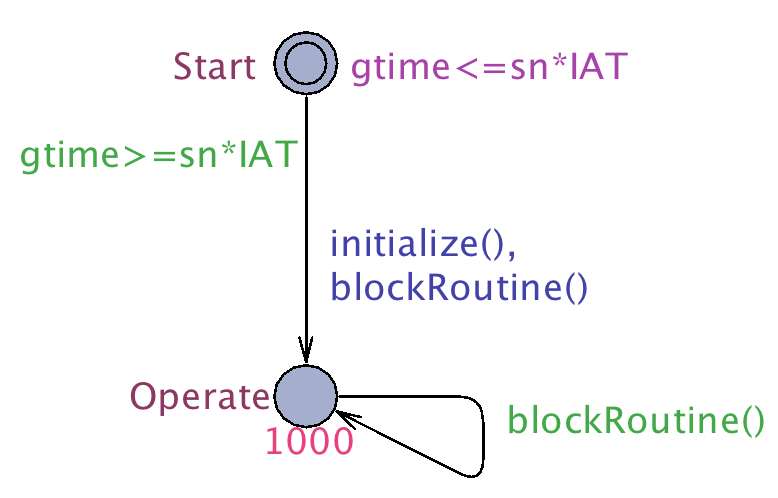
\includegraphics[width=0.45\textwidth]{images/continuous-sta}
	} ~
	\subfloat[Discrete-time.\label{fig_discrete}]{% 
		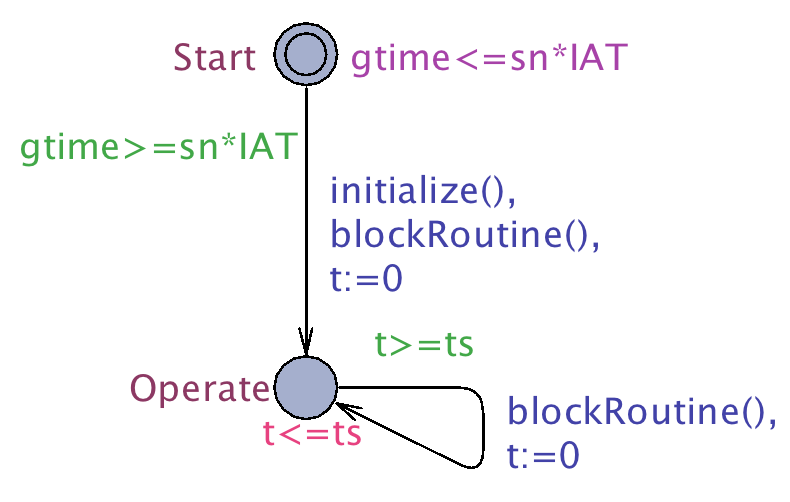
\includegraphics[width=0.45\textwidth]{images/discrete-sta}
	} 
	\caption{STA transformation patterns.} 
	\label{fig_patterns}
\end{figure}

\subsection*{Simulink to NSTA Transformation Process} 
Besides proposing the transformation patterns, we provide an automatic transformation of a Simulink model to its equivalent network of STA by applying the following tasks:
\begin{enumerate*}[label=(\roman*)]
	\item the Simulink model is simulated, subsequently, the sorted-order list, which contains the execution order of the Simulink blocks, is extracted;
	\item in case the model is hierarchical, the execution order is flattened first, thus generating a flattened sorted-order list;
	\item the Simulink model is parsed, as a result, each block is translated into a stochastic timed automaton via the corresponding transformation pattern. The sorted-order number $sn$ is instantiated from the sorted-order list on the fly;
	\item any non-computation blocks is accounted in the transformation but is not transformed into an automaton; examples of such blocks are Mux, SubSystem blocks etc.;
	\item the connections between the blocks are translated into global variables, which act as the communication means between the automata.
\end{enumerate*}
For details on the transformation, as well as on the soundness proof for discrete-time models, the reader is invited to consult Paper D~\cite{Filipovikj2018SimppaalModels}

%\begin{figure}
%	\centering
%	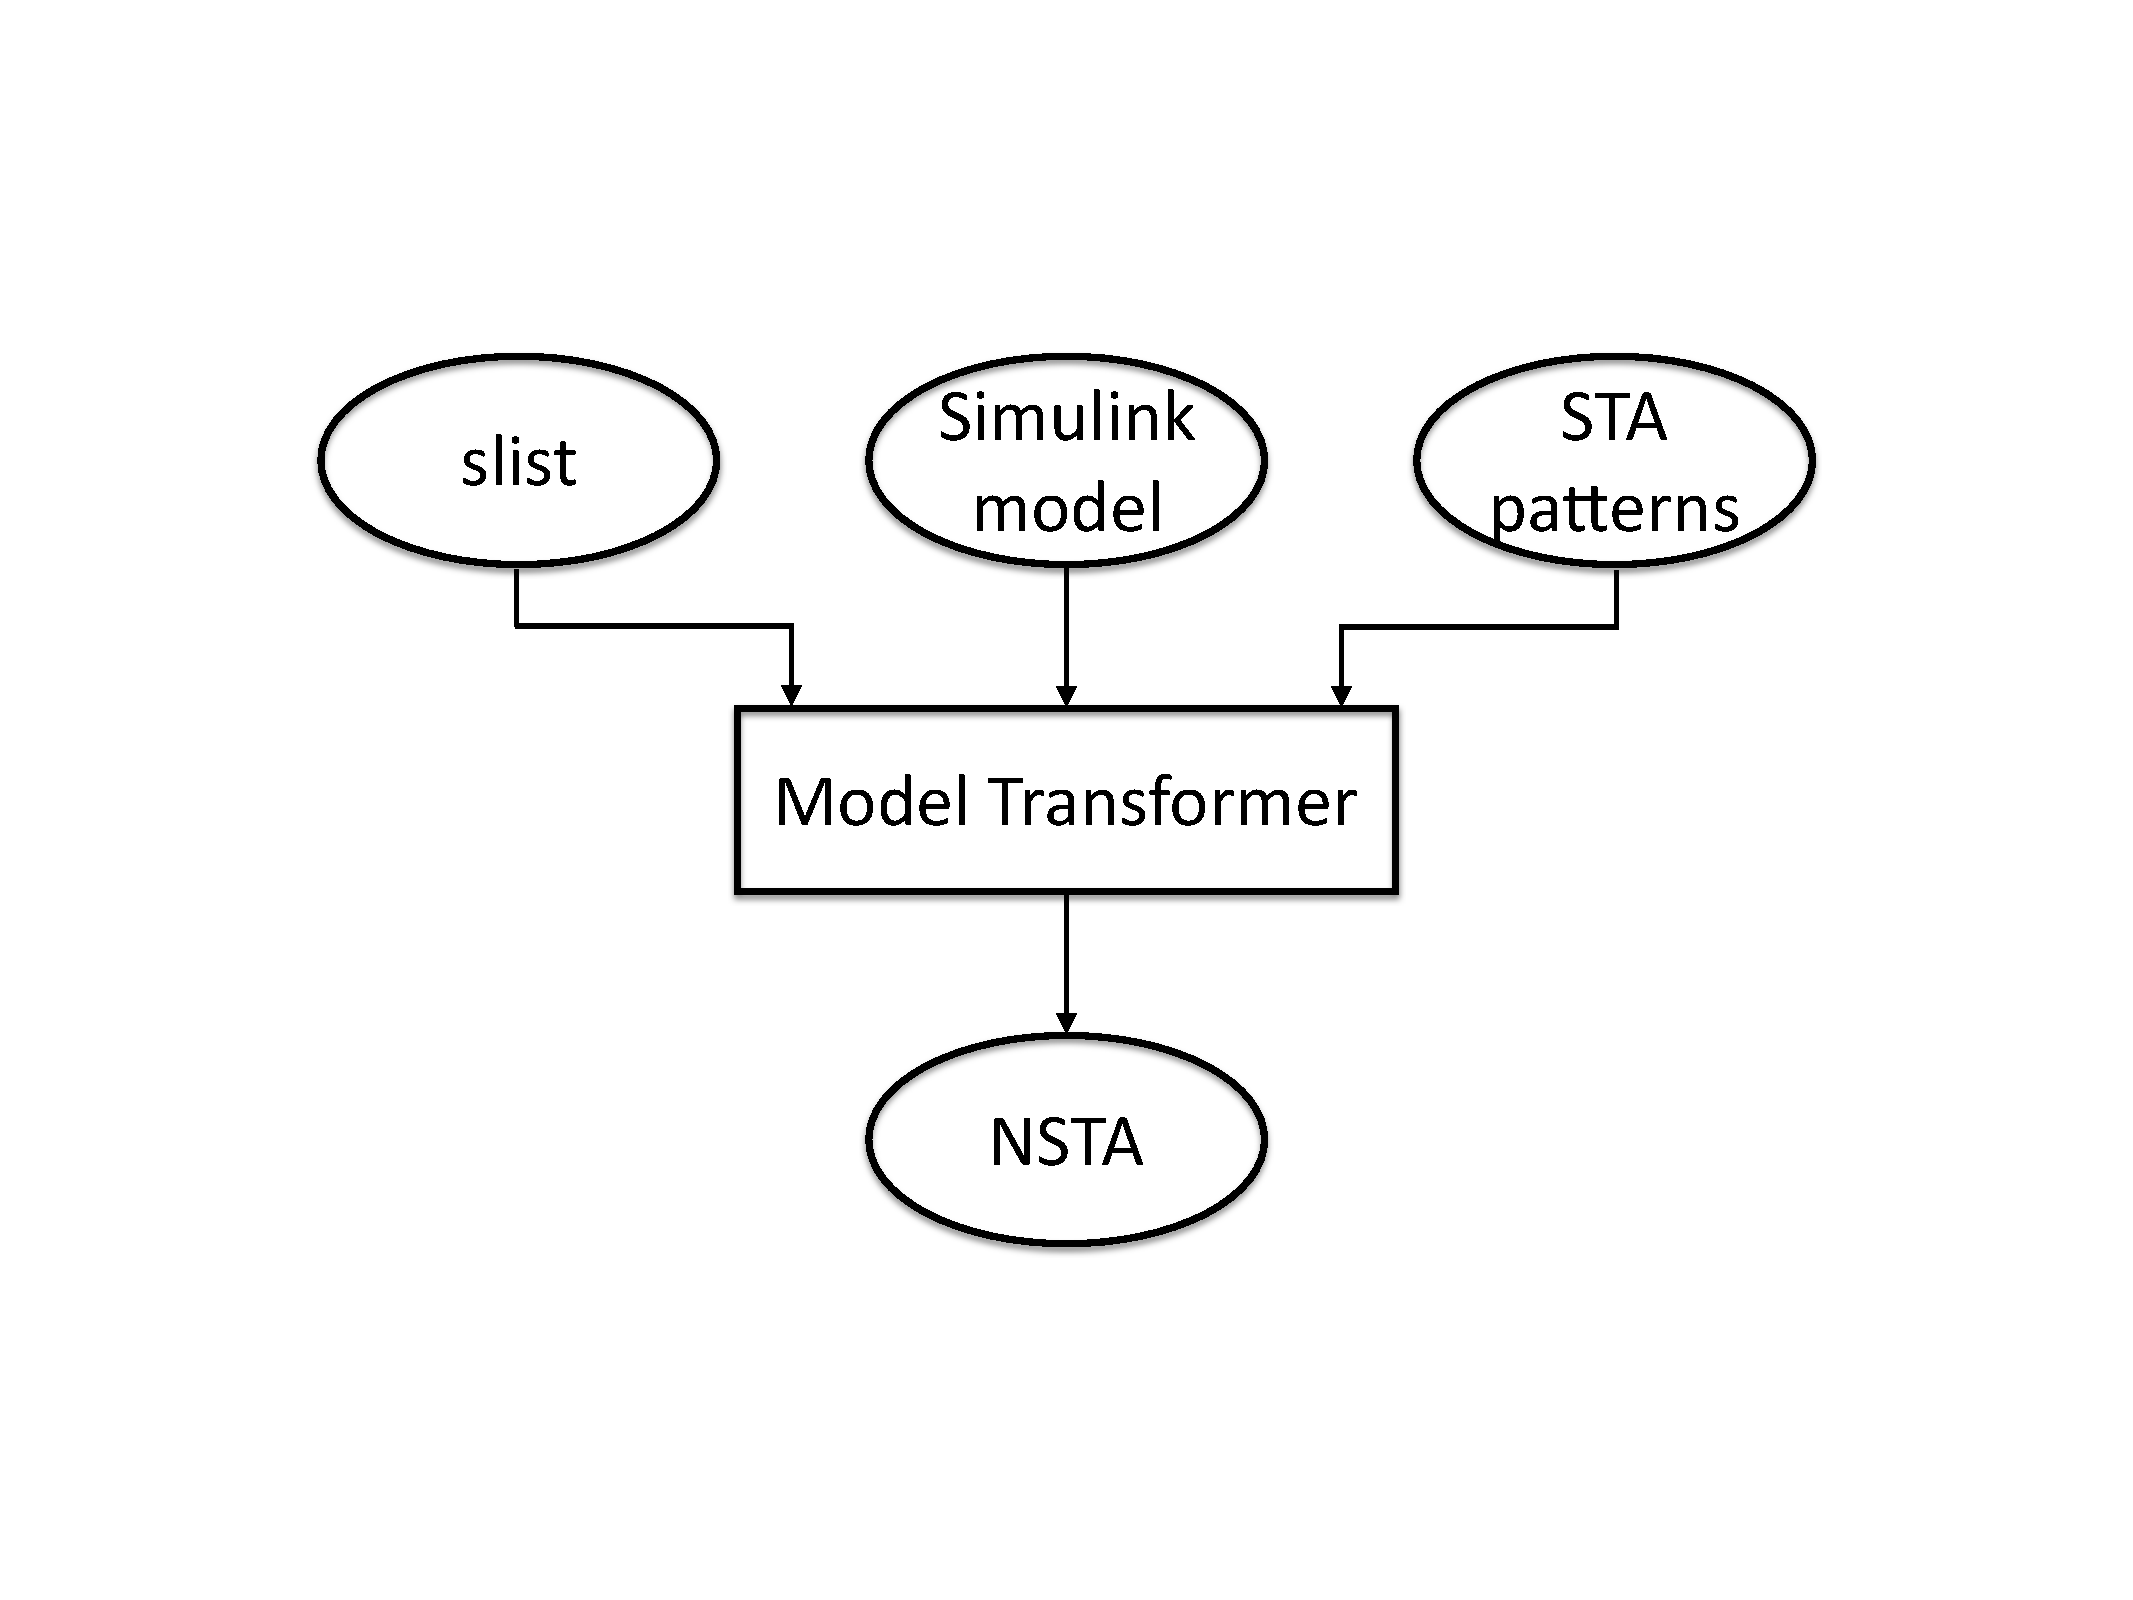
\includegraphics[width=0.6\linewidth]{images/simulinkapproach}
%	\caption{Simulink to NSTA Transformation}
%	\label{fig_approachworkflow}
%\end{figure}

\subsection*{Validation on the Brake-by-Wire Use Case} 
Our approach is applied on an industrial Brake-by-Wire Simulink model, which is a prototype developed for academic use by VGTT. The model consists of 320 blocks, of which 19 are discrete blocks, 26 constant blocks and the rest are continuous blocks. The model design consists of modules that collect sensory data, e.g., vehicle speed, pedal position, and compute the proportional torque force that is applied on the wheels to brake the vehicle. Besides, it has the  anti-braking functionality (ABS) to avoid (or minimize) skidding, which occurs when the slip rate of a wheel is greater than its friction coefficient. 

The BBW requirements are initially specified in \resa, subsequently are translated into PWMTL properties manually by using monitors (or observers), which are stopwatch stochastic priced timed automata. The monitors are modeled for particular requirements, and basically observe the progression the execution of the automata.
\begin{example}[Statistical model checking of BBW]\label{ex_resa}
	The BBW model is automatically transformed into a network of STA, and we model monitors~\cite{Filipovikj2018SimppaalModels} to represent 5 functional and timing requirements, out which 3 requirements are shown in the box below for illustration. 
	\vspace{0.2cm}
\begin{elaboration}{0.9}
	\small
	{}
	\begin{tabular}{lp{.85\textwidth}}
	R1 & The brake request shall be computed within 10 ms. \\
	R3 & The brake request shall be propagated to two different wheel actuators within 4 ms.\\
	R4 & If the brake request is 0, then the ABS shall set the torque to 0. \\
\end{tabular}
\end{elaboration}
\end{example}

Figure~\ref{fig_smcresult} shows the PWMTL properties and their model-checking results. R1 and R3 as presented in the able above  are safety requirements expressed using the $\Box$ (always) operator in their formal counterpart, as indicated by R1$_{BBW}$ and R3$_{BBW}$ PWMTL properties of Figure~\ref{fig_smcresult}. R4 is a conditional requirement expressed using the $\Diamond$ (eventually) operator in its formal translation, as encoded by the R4$_{BBW}$ PWMTL property. Each result in Figure~\ref{fig_smcresult} shows the probability interval of satisfying the property (qualitative), confidence level, the number of runs and the time needed by the model checker to return the result. For some properties in Table~\ref{fig_smcresult}, the probability interval of satisfying the respective property is $[0.99, 1]$, which can be considered as ``property satisfied'' if the lower bound on the probability is 0.99. However, in many safety-critical applications, the requirement on the probability is normally high, e.g., 0.999999 (essentially approximates to ``no failure should happen''). In this case, the interval should be more precise, which can be achieved by lowering $\alpha$ and $\beta$ of the hypothesis testing, which are probabilities of accepting false positives, and false negatives, respectively~\cite{David2011StatisticalAutomata}.
\begin{figure}
	\centering
	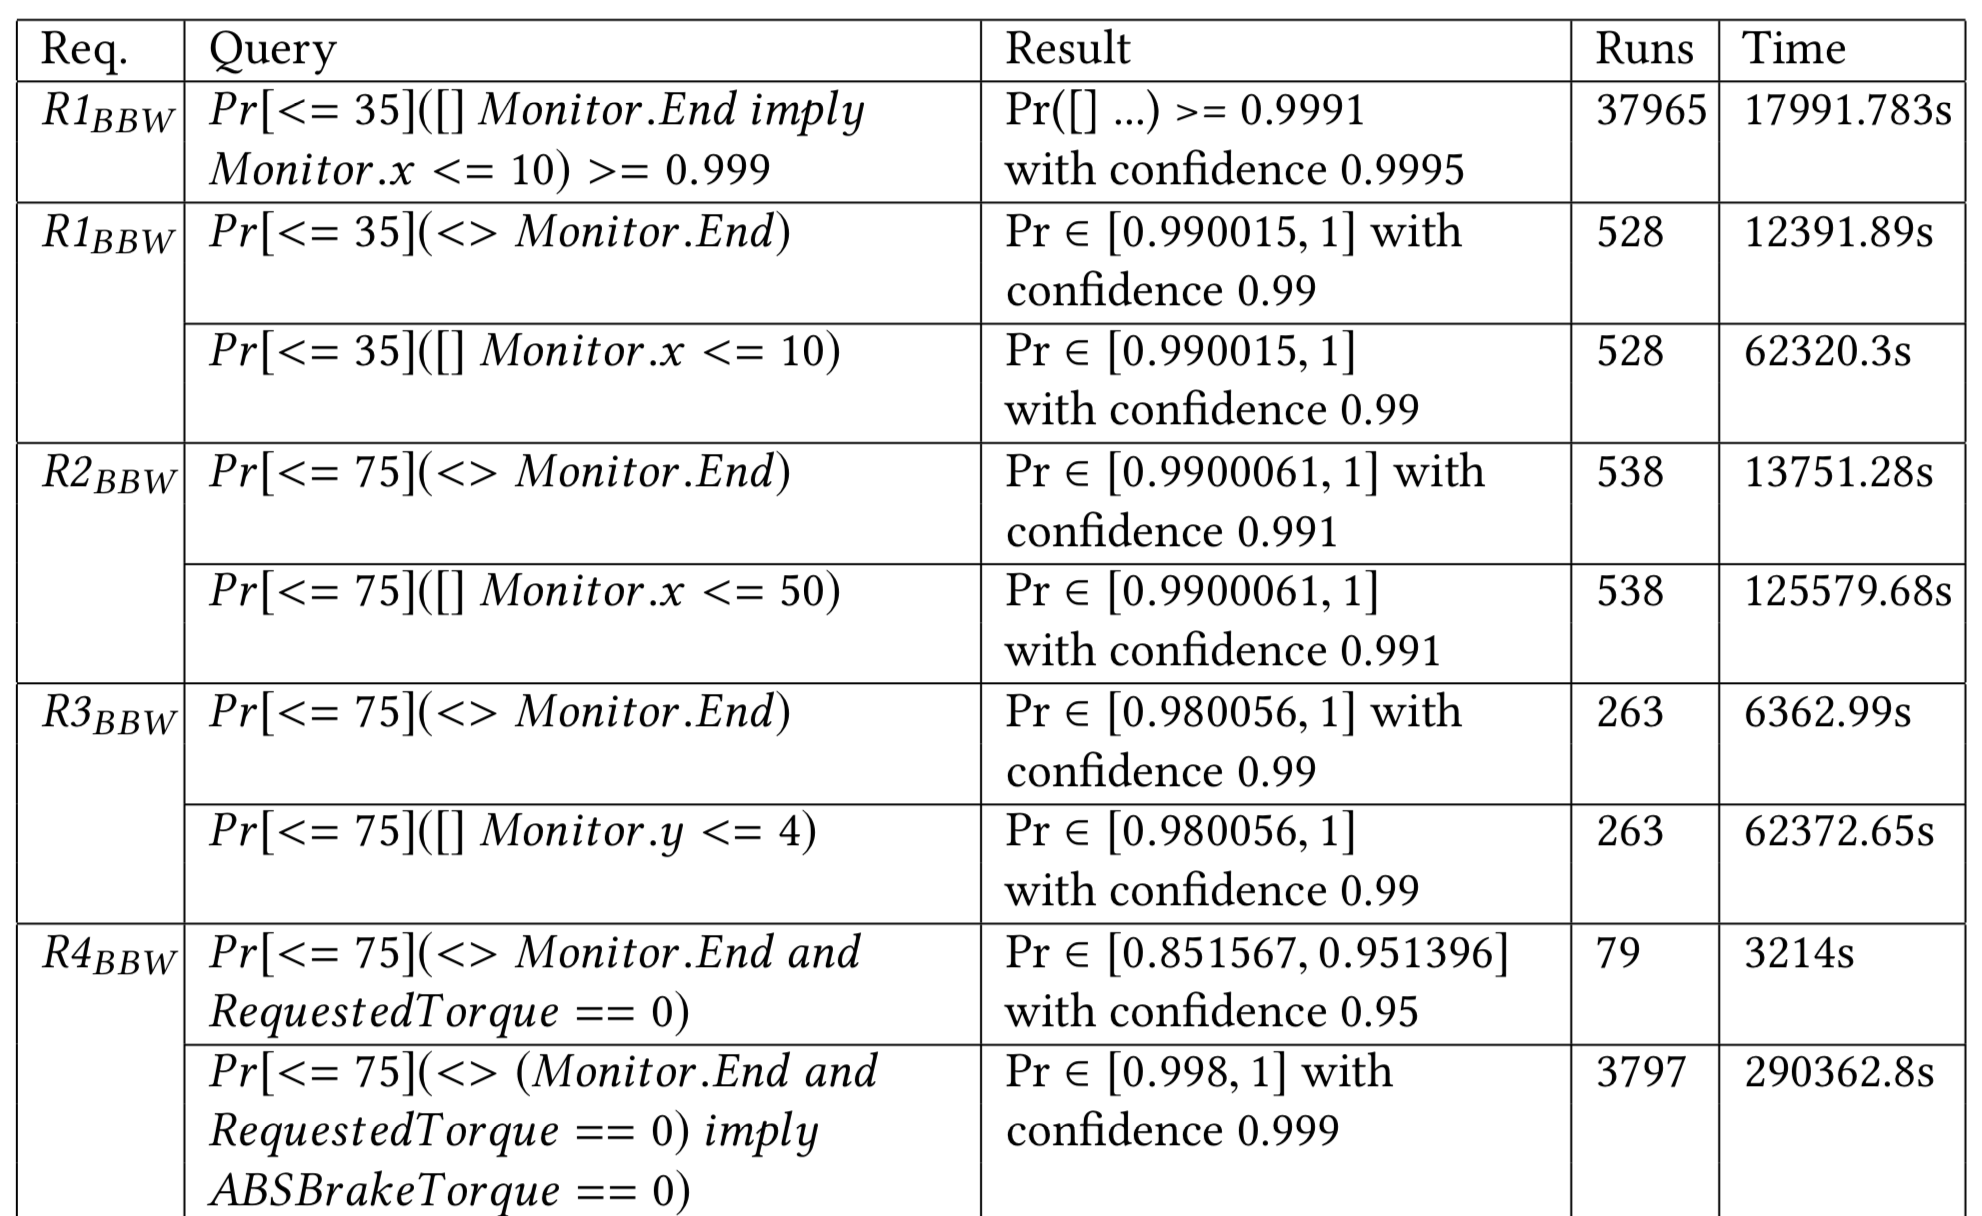
\includegraphics[width=1\linewidth]{images/smc_result}
	\caption{Analysis results snippet of the BBW Simulink model from \uppaalsmc{}. For the complete results, we refer the reader to~\cite{Filipovikj2018SimppaalModels}.}
	\label{fig_smcresult}\vspace{-0.2cm}
\end{figure}

\section{RC4: Fault-tolerant Software Allocation}\label{rc_ilp}
In this thesis, we have proposed two software allocation approaches based on integer linear programming (ILP) and hybrid  particle swarm optimization (PSO) optimization algorithms. The system model is briefly described as follows. We consider an \autosar{} safety-critical software application that can be mapped to multiple computing nodes, which are heterogeneous with respect to power specification, failure rate and processing speed. The software application has end-to-end timing and reliability requirements, which must be satisfied by the mapping solution. In order to meet the reliability requirement, the allocation applies fault tolerance by replication of software components, which are mapped to different computing nodes. We assume the nodes failures are mutually exclusive and permanent, and the replication is active, hence no time between failures is assumed.

The software application is modeled as directed acyclic graph (DAG), where the nodes are runnables and the links are communications between the runnables. A cause-effect chain (or chain) is a sequence of runnables that realize some software functionality, e.g., the pressing of a brake pedal (the cause) and the slow down of a vehicle (i.e., the response). Before the allocation begins, the runnables are mapped to tasks using merging rules according to the \autosar{} methodology. The tasks and messages that realize the safety-critical software functionality are scheduled using a fixed-priority preemptive scheduling policy~\cite{Sha2004RealPerspective} and fixed-priority non-preemptive scheduling policy (over a  CAN bus), respectively. We assume that the runnables are triggered periodically and have multiple worst-case execution times for the different processors.

\subsection*{Allocation via Integer Linear Programming}
Consider that the mapping solution is represented by a vector of binary matrices $\textbf{x}=\{\textbf{x}_1:1,...,K\}$, where \ttxkij{} represents the mapping of the software component $q^{k}_{ij}$ to the computing node $\ssb{n}[j]\in \mathcal{N}$. 
\begin{equation}
\label{eqn_solution}
\bspx{k}=
\begin{bmatrix} 
\ssx{k}{11} & \ssx{k}{12} & \dots & \ssx{k}{1K}\\
\ssx{k}{21} & \ssx{k}{22} & \dots & \ssx{k}{2K}\\
\vdots & \vdots & \ddots & \vdots\\
\ssx{k}{N1} & \ssx{k}{N2} & \cdots & \ssx{k}{NK}
\end{bmatrix}
\end{equation}

The power consumption of a software application that is mapped to computing units $N'\in N$ is calculated as the sum of the power consumption of each node $n_h\in N'$, i.e., $\mathcal{P}_{total}(x)=\sum_{n\in N'}{\mathcal{P}(u_n(x))}$, where $\mathcal{P}(u)$ is the power consumption of a computing node which is linearly proportional to its utilization~\cite{Mahmud5222}. The utilization of a computing node is the sum of the utilization of its constituent tasks (or software components). Equation (\ref{eqn_isp_util}) computes the utilization of the nodes.
\begin{align}
\label{eqn_isp_util}
	(u_1,...,u_K)(\x)=\sum_{k=1}^{K}\sum_{\tau\in T_{c_i}}{\xkij*\frac{C_\tau}{P_\tau}},
\end{align}
where $T_{c_i}$ is the set of tasks which realize the software component $c_i$ (which is a type for $q^{k}_{ij}$ replica), $C_\tau$ and $P_\tau$ are the worst-case execution time and  period of the task $\tau$, respectively.

We apply the classical worst-case response time analysis~\cite{Baruah2011Response-timeSystems} to check the schedulability of tasks sets in each node. The analysis is recursive, and depends on a higher priority tasks set, which is dynamic for different mappings. The end-to-end delay of a chain is calculated for data age (also known as age delay), which is iterative. Thus, we propose a formulation of the timing constraints as logical linear constraints as follows: (i) we identify the the software components partitions $P=2^C$, where $p\in P$ can be mapped to a node; (ii) we check the schedulability of each partition in each node $Y_j=\{p\in P| isSched(p,n_j)\}$, where $sched$ is a Boolean predicate that returns \textbf{true} if $p$ is schedulable on $n_j$.  A partition is identified by a sequence of 0s and 1s based on its constituent components, e.g., the id of the partition $\{c_1,c_4,c_5\}\subseteq \{c_1,c_2,c_3,c_4,c_5\}$ is $10011=19$. So, given the mapping $\x$, the partition id that is mapped to the computing node $n_j$ can be computed as
\begin{align}
	g_j(\x)=\sum_{i=1}^{N}{10^{N-i}\max_{1\leq k< K}\xkij}
\end{align}
where the $\max_{1\leq k< K}$ function returns 1 if at least one component replica is mapped to $n_j$ otherwise returns 0, indicating no replica is mapped to that node. Thus, each node must have a valid partition that is schedulable as indicated in the logical constraint,
\begin{align}
\bigvee\limits_{p\in Y_j}g_j (\x)= id(p) ,
\end{align}
where $id(p)$ is a predicate that returns the id of the partition $p$.

Similar to the tasks deadline constraints, we construct logical constraints that correspond to the valid set of chains. Given $\Gamma =\{\Gamma_i:i=1,...,N\}$ chains, the set of possible mappings of each chain $\Gamma_i$ on a set of $\mathcal{N}$ nodes is ${\Gamma_i}^\mathcal{N}$. Thus, the set of valid mappings of each chain that satisfy the end-to-end timing requirements are $Z_i=\{\gamma\in {\Gamma_i}^\mathcal{N}| ageDelay(\gamma) \leq {EE}_\gamma$.

The reliability constraint refers to the probability that the application functions by the time $t$, i.e $[0,t]$~\cite{Goel1985SoftwareApplicability}. % We assume that the reliability requirement of a software application is 0.99999999 over a 2-year operation time, which is to say  that the safety-critical system almost should not fail within the stated period. Furthermore, we assume that the mean-time to failure of the computing nodes is given as $10^6$ hours (0.0000001 per hour), which is the usual practice in many functional safety design.
Unless the the software application is replicated on one or more computing nodes, the reliability requirement is usually unattainable. So, the allocation strategy is basically to replicate sufficient software components to meet the requirement. However, the reliability calculation is not trivial as the replication results in functional inter-dependency of the computing nodes due to the replication of components, in which case, the series-parallel method does not always apply. Instead, we propose an exact method based on state enumeration~\cite{Lucet1999ExactReliability} of the computing nodes, i.e., all the possible configurations of the nodes $PS$ are enumerated. Subsequently, the reliability of the application is computed as the total probability of those configurations that allow functioning of the application~\cite{Mahmud5222}.
%, which is defined by its inverse as follows:
%\begin{definition}[Software Application Failure]
% 	A software application fails in the configuration $s\in\xi$ if there exists a component type $c_i$ where all of its replicas $Q_i$ \textit{fail}, otherwise, it functions, as determined by Equation (\ref{eqn_appreliability_milp_components}) using the floor function. The component replica $q_{ij}\in Q_i$ of type $c_i$ fails if $n_h$ fails, that is $s_h=0$. For instance, $s=101$ denotes the nodes $n_1$ and $n_3$ functions and node $n_2$ fails. 
% \end{definition}
% \begin{align}
% f_s(x) = \floor[\Bigg]{\frac{\sum_if_{c_i}(x,s)}{N}}=
% \begin{cases}
% 1 & \mbox{if } application \mbox{ functions}\\
% 0 & \mbox{if } application \mbox{ fails}
% \end{cases}\label{eqn_appreliability_milp_components}
% \end{align}h

% Thus, the reliability of the software allocation is
% \begin{align}
% \label{eqn_appreliability_milp}
% Reliability(\x)=\sum_{s\in PS}f_s(\x)*p_s,
% \end{align}
% where $p_s$ is the probability that the computing nodes attain a configuration $s$ which is computed as $p_s=\prod_{m\in M}\big[(z_m*\lambda_m) + (1-z_m)*(1-\lambda_m)\big]$, where $z_m\in\{0,1\}$ indicates if the node fails (i.e., 0) or functions (i.e., 1), $\lambda_m$ is the failure rate of the node $m$ and $1-\lambda_m$ is the opposite of failure rate, i.e., that is the rate that it does not fail.


%The ILP optimization goal is to minimize the total power consumption, which is the objective function, and the constraints Equation (\ref{lbl_deadline_constraint}), (\ref{lbl_e2e_constraint}) and (\ref{lbl_reliability_constraint})ensure that the optimization satisfies the tasks deadline, end-to-end timing and reliability constraints, respectively.
% \begin{align}
% \label{eqn_const_func}
% \min_{\x\in X} \mathcal{P}_{total}(\x) && \text{ Subjected to:}\\
% \label{lbl_deadline_constraint} 
% \bigvee\limits_{p\in Y_j} g_j (\x) &= id(p)& \mbox{ for all } j=1,..,|\mathcal{N}|\\ 
% \label{lbl_e2e_constraint}
% \bigvee\limits_{\gamma\in Z_j} h_j (\x) &= id(\gamma) & \mbox{ for all } j=1,..,|\Gamma|\\ 
% \label{lbl_reliability_constraint}
% \sum_{s\in PS}f_s(\x)*p_s &\leq \RL&,
%   \end{align}


\section*{Allocation via Hybrid Particle Swarm Optimization}\label{rc_pso}
In this section, we propose approximation algorithms based on metahuristics, which is ``high-level problem-independent algorithmic framework that provides a set of guidelines or strategies to develop heuristic optimization algorithms''. Meta-heuristic algorithms does not guarantee optimality of solutions, nevertheless, the solutions can be deemed satisfactory. In the case of minimizing power consumption, what is more appealing to system designers is usually the benefit attained as a result of the power consumption reduction, e.g., accommodating more and more software applications, improving battery-life, rather than optimality. In this spirit, metahuristics can be useful to solve complex and large optimization problems, yet in reasonable time, as compared to exact methods, e.g., branch-and-bound, dynamic programming.

%\subsection*{Hybrid Particle-swarm Optimization}
The canonical \pso{} technique uses the constriction factors to balance exploitation and exploration of the search space to get closer to the global optima, hence improving solution quality. Nevertheless, it still suffers from premature convergence or local minima especially when applied on complex and large problems~\cite{Rini2011ParticleChallenges}. Its hybridization is proven to perform better in many cases~\cite{Sengupta2018ParticlePerspectives}. In particular, it is shown to perform better in the tasks assignment problem, that is when hybridized with, e.g., the genetic algorithm~\cite{Sailer2013OptimizingAUTOSAR}, the hill-climbing~\cite{yin2007task}, simulated annealing~\cite{Zhao2007ASystem}, differential evolution~\cite{Storn1997DifferentialSpaces}. As compared to the hybridization with genetic, the hybridization with hill-climbing \hcpso{} is shown to perform better~\cite{yin2007task} for the tasks allocation problem to maximize reliability of distributed systems. 

In this work, we apply \hcpso{} and its stochastic version \shpso{} to the problem at hand, in order to tackle the \pso{} stagnation when applied to large and complex problems. Moreover, we hybridize \pso{} with the differential evolution technique, \depso{}, to improve diversification by applying the mutation and cross-over operators of the differential evolution. Algorithm~\ref{alg_depso} shows the pseudocode of the hybrid \pso{}. Line 3 and 4 compute the personal best and the swarm best solutions, respectively. For each particle in the swarm, the velocity and position is computed in Lines~5-8. Lines~9-13 apply the hybridization based on the choice of the algorithm, i.e. \de, \hcpso{} and \shpso{}, intermittently, i.e., whenever the \textit{interval criterion} condition satisfies.
\IncMargin{1em}
\begin{algorithm}[H]
	\SetAlgoLined
	\SetKwData{P}{P}\SetKwData{S}{sBest}
	\SetKwData{Generation}{Generation}
	\SetKwData{Interval}{Interval}
	\SetKwData{Particles}{Particles}
	\SetKwInOut{Input}{input}\SetKwInOut{Output}{output}
	\SetKwFunction{OptimizeUsingDE}{optimizeUsingDE}
	\SetKwFunction{OptimizeUsingHC}{optimizeUsingHC}
	\SetKwFunction{OptimizeUsingSHC}{optimizeUsingSHC}
	\SetKwFunction{ComputeParticleVelocity}{computeParticleVelocity}
	\SetKwFunction{ComputeParticlePosition}{computeParticlePosition}
	\SetKwFunction{InitPSO}{initPSO}
	\SetKwFunction{ComputePersonalBest}{ComputePersonalBest}
	\SetKwFunction{ComputeSwarmBest}{ComputeSwarmBest}
	
	\BlankLine
	\Input{\pso parameters, \de parameters}
	\Output{Software allocation solution \S .\textbf{x}}
	\BlankLine
	\Particles $P$ $\leftarrow$ \InitPSO{}\;
	\BlankLine
	\While{termination criteria}{
		$\textbf{p}_{bst}$ $\leftarrow$\ComputePersonalBest{$P$}\;
		$\textbf{z}\leftarrow$\ComputeSwarmBest{$P$}\;
		\BlankLine
		\ForEach{$p\in P$}{
			\ComputeParticleVelocity{$p$} according to Equation (\ref{eqn_pso_velocity})\;
			\ComputeParticlePosition{$p$} according to Equation (\ref{eqn_pso_position})\;
		}
		\If{interval criteria}{
			$P$ $\leftarrow$ \OptimizeUsingDE{$P$}\;
			\tcp{$P$ $\leftarrow$ \OptimizeUsingHC{$P$}}\label{hc}
			\tcp{$P$ $\leftarrow$ \OptimizeUsingSHC{$P$}}\label{sh}
		}
	}
	\caption{Hybrid \pso{} Pseudocode.}
	\label{alg_depso}
\end{algorithm}\DecMargin{1em}

\subsection*{Validation on the Bosch EMS Benchmark}
Our proposed software allocation approaches are validated on different sizes of software applications, i.e., applications with variable number of software components, cause-effect chains and degree of replication. The applications are synthesized according to the automotive benchmark proposed by Kramer et al.~\cite{Kramer2015RealFree}, which contains the timing specifications of runnables and their shares in the AUTOSAR implementation of an engine management system (EMS). Moreover, it shows the activation patterns of cause-effect chains, number of runnables per activation and their shares in the system. The engine management system is one of the most complex automotive systems in the vehicular electrical/electronic platform. 

\noindent\textbf{The ILP approach validation: }we have prepared 7 software applications and an execution platform that consists of 8 nodes. The smallest application consists of 4 components and the largest application 10 components. Furthermore, the cause-effect chains vary from 10 to 60, the activation patters range from 2 to 4, which are consistent with the benchmark specifications.
    
Figure~\ref{fig_ilp_results} shows the result of the \ilp{} optimization as solved by the \cplex{} solver. The algorithm selects the computing nodes with the lower power specifications as more resources are needed as more components are allocated. Note that, the figure legend shows a list of nodes listed in ascending order according to power consumption specifications. Figure~\ref{fig_computationtime_ilp} shows a marginal increase of computation time until the number of components hits 8, which took 6.06 sec. Afterwards, it rapidly increases to 30.3 sec and 129.4 sec for allocating 9 and 10 components, respectively. The optimization took large amount of time to allocate 15 components, and extremely large computation time to allocate beyond 15, consequently interrupted manually. For more of the validation results and analysis, refer Paper D~\cite{Mahmud5222}.
\begin{figure}[h] 
	\centering
	\subfloat[Power consumption of nodes.\label{fig_powerconsumption_ilp}]{% 
		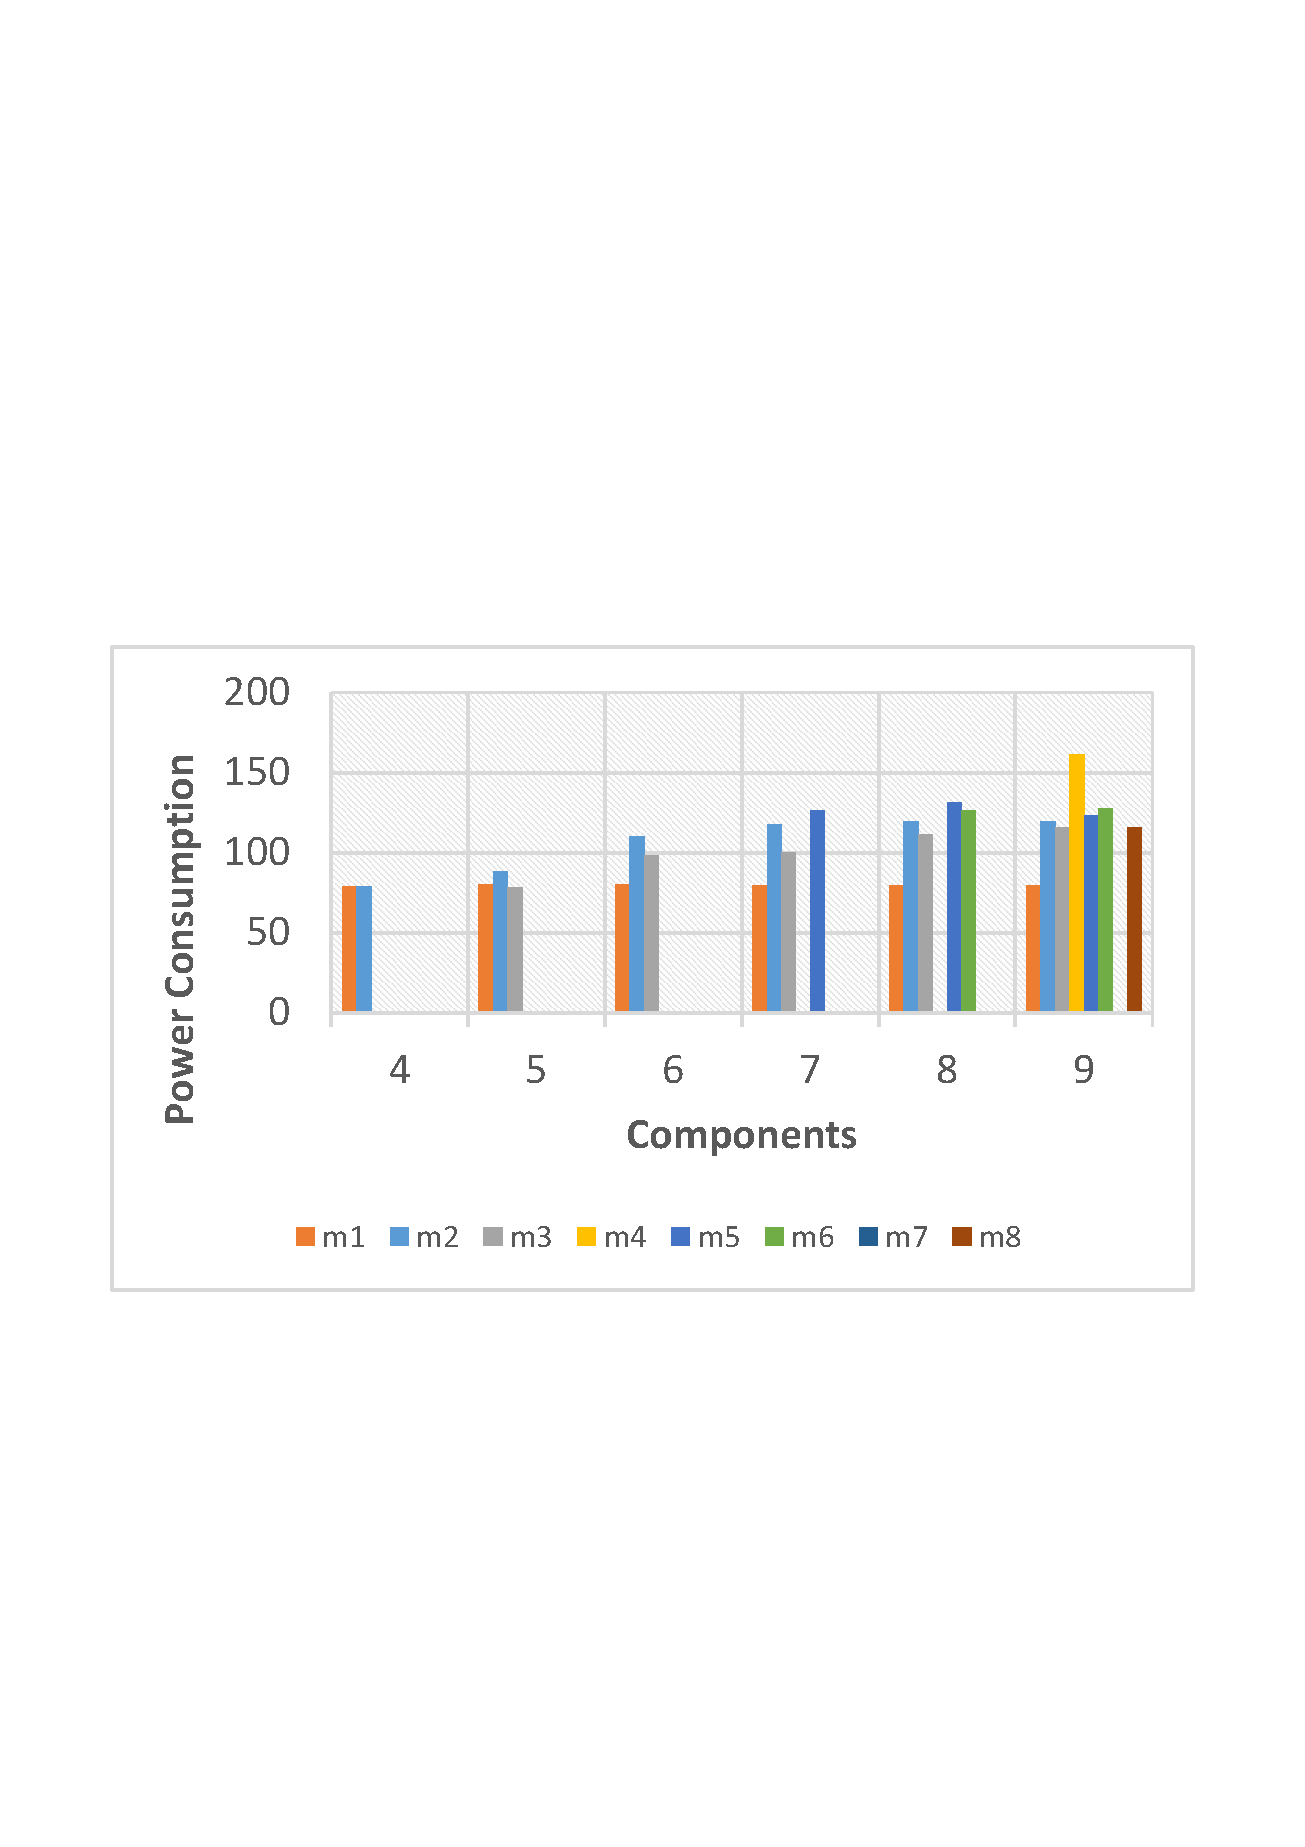
\includegraphics[width=0.45\textwidth]{images/power}
	} ~
	\subfloat[Computation times for software allocations. .\label{fig_computationtime_ilp}]{% 
		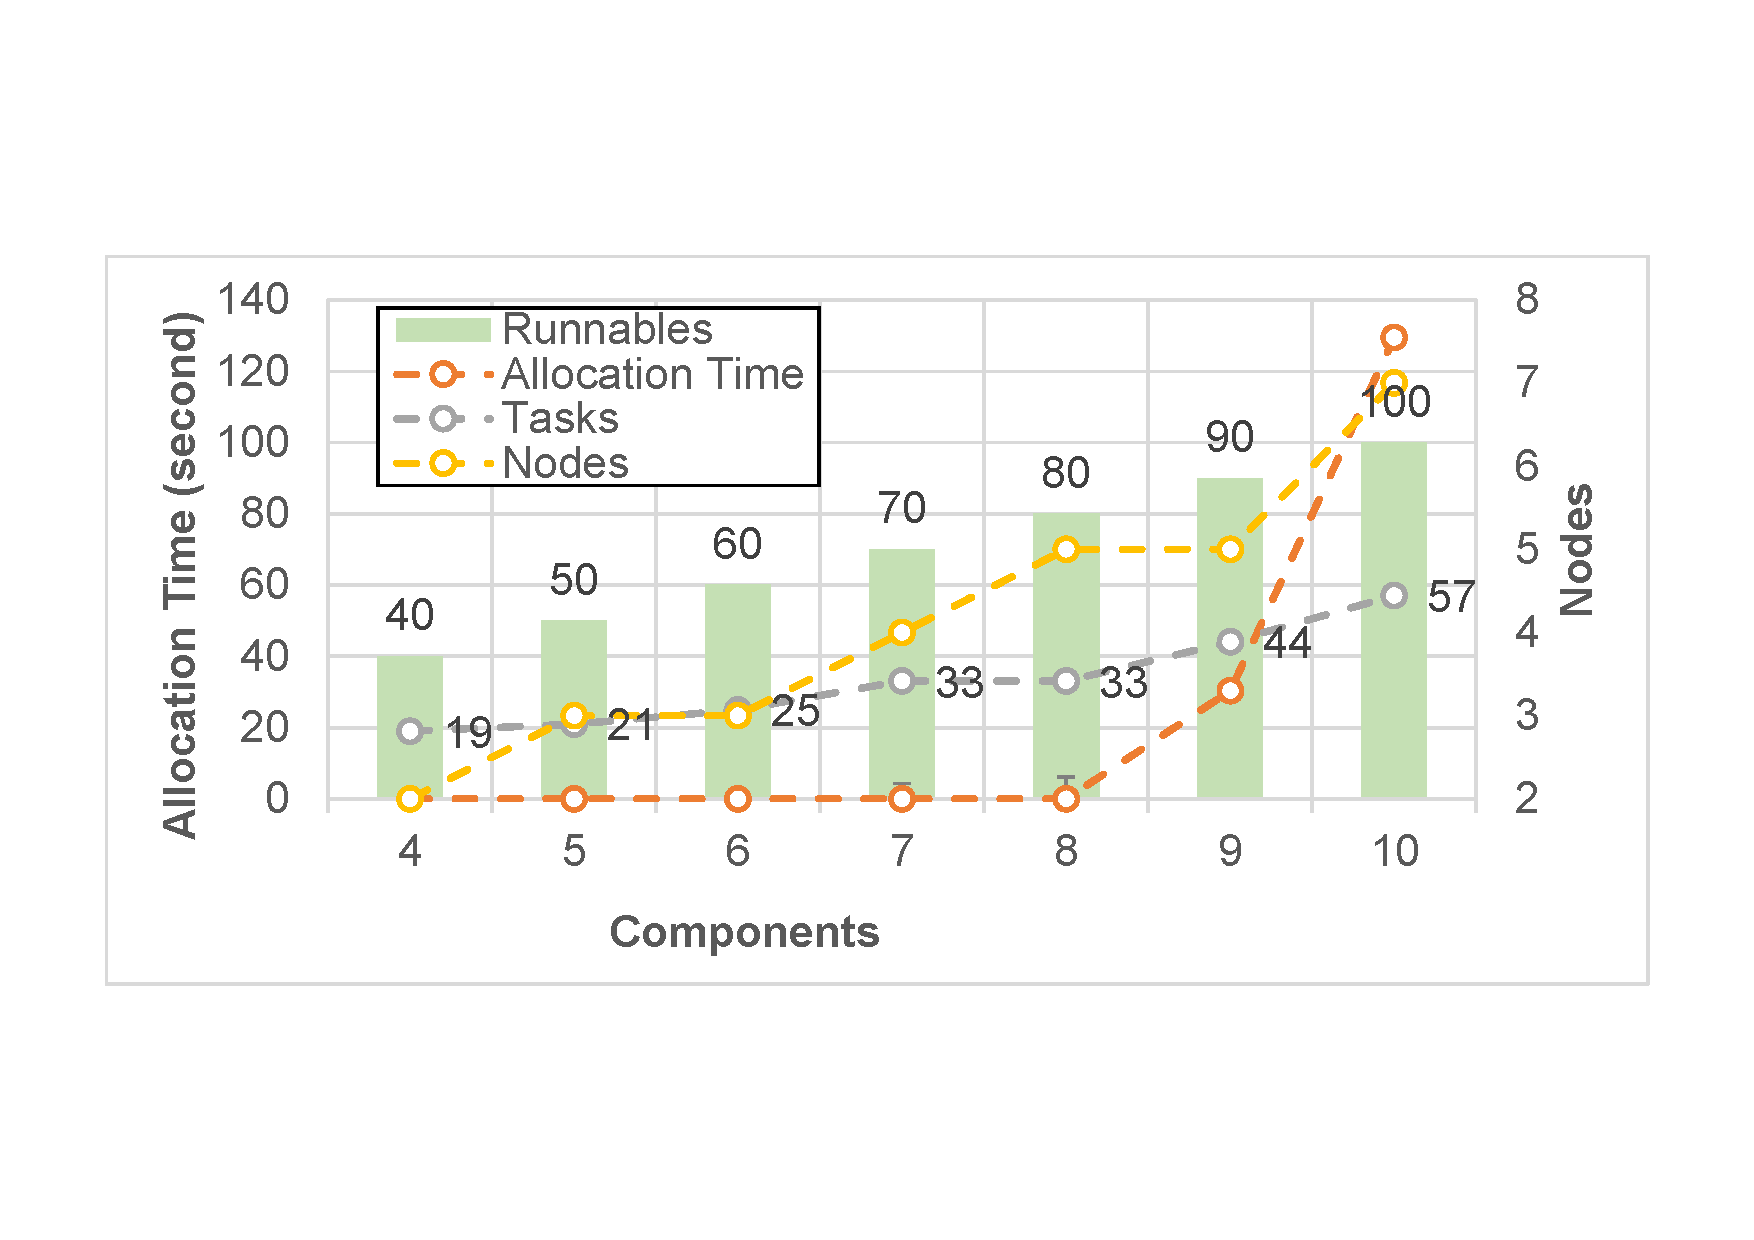
\includegraphics[width=0.55\textwidth]{images/increasing_components} 
	} 
	\caption{ILP optimization of different sizes of software applications based on the number of software components, cause-effect chains, computing nodes.} \label{fig_ilp_results}
\end{figure}

\noindent\textbf{The hybrid PSO approach validation: } we have prepared 7 software applications, which are identified by $\langle cimjgk\rangle$, where $c,m,g$, respectively, refer to the components, computing nodes and chains, and $i,j,k\in\mathbb{I}^+$, respectively, refer to the cardinality of $c,n,g$, respectively, in the application.

As opposed to the ILP approach, in this validation, we have to consider quality of the solutions since the solutions delivered by meta-heuristic algorithms do not guarantee optimality. Furthermore, we evaluate the impact of the proposed approximation algorithm to minimize the overhead of the replication on the optimization. 

Figure~\ref{fig_powerconsumption_ilp_metaheuristic} shows \ilp{} and all except \pso{} and \depso{} return optimal solutions in the first three problems. However, as the problem size increases, the hybrid PSO with the local search algorithms, i.e. \hcpso{} and \shpso{}, deliver better solutions as compared to \depso{}. 
% \begin{figure}
% 	\centering
% 	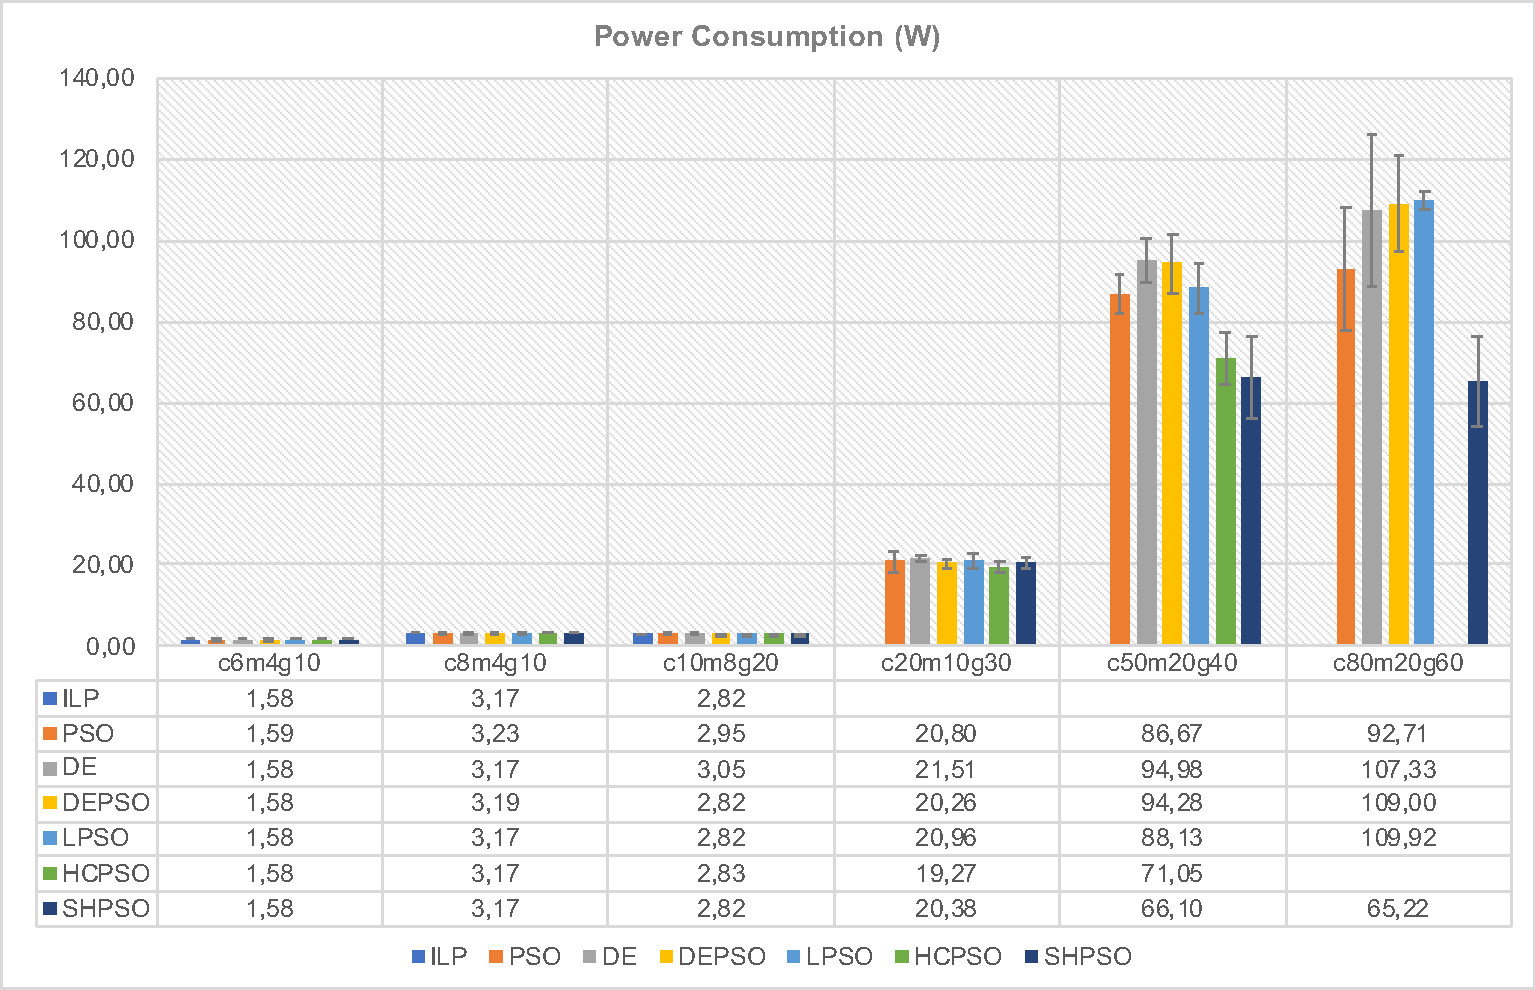
\includegraphics[width=0.8\linewidth]{images/power_consumption.pdf}
% 	\caption{Power consumption of nodes for different instances of software allocation problems by different optimization algorithms.}
% 	\label{fig_powerconsumption_ilp_metaheuristic}\vspace{-0.4cm}
% \end{figure}
\begin{center}
\resizebox {0.9\textwidth} {!} {
\begin{tikzpicture}[spy using outlines={circle,black,magnification=1.75,size=1.25cm, connect spies}]
\node {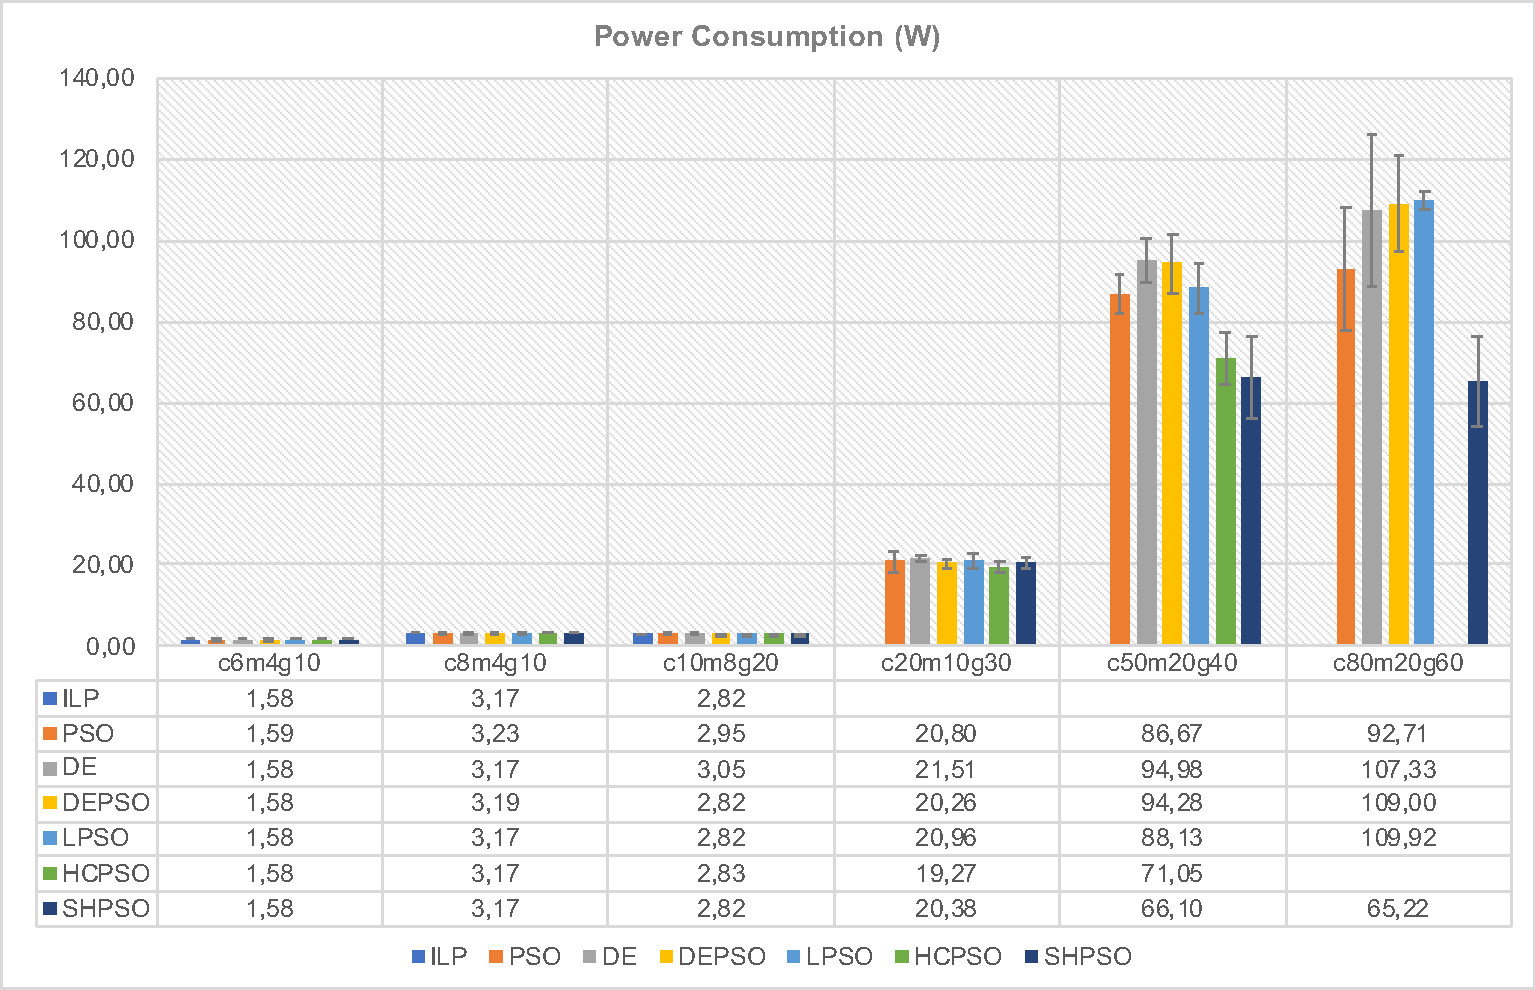
\includegraphics[width=1\linewidth]{images/power_consumption.pdf}};
\spy on (-2.1,-1.2) in node [draw,thin, ellipse, minimum width=9cm, minimum height=1.25cm,align=left] at (0,2.70);
\end{tikzpicture}}
\end{center}

Figure~\ref{fig_allocationtime_ilp_metaheuristic} shows that the hybrid \pso{} algorithms with local search perform the best in the last three problems except \hcpso{}, which fails to return near optimal solutions to the largest problem \pb{80}{20}{60} due to extremely large computation time, consequently manually interrupted. Thus, the stochastic version of the hill-climbing algorithm scales well, and its overall quality of the solution can be deemed acceptable as compared to \ilp{} or \hcpso. The analysis of the approximation algorithm that is introduced to lower the overhead of replication on the end-to-end computation has resulted in lower computation time, as expected, while impacting less the quality solutions. For more of the validation results and analysis, refer Paper F~\cite{Mahmud2019OptimizedConstraints}.
\begin{figure}[h]
	\centering
	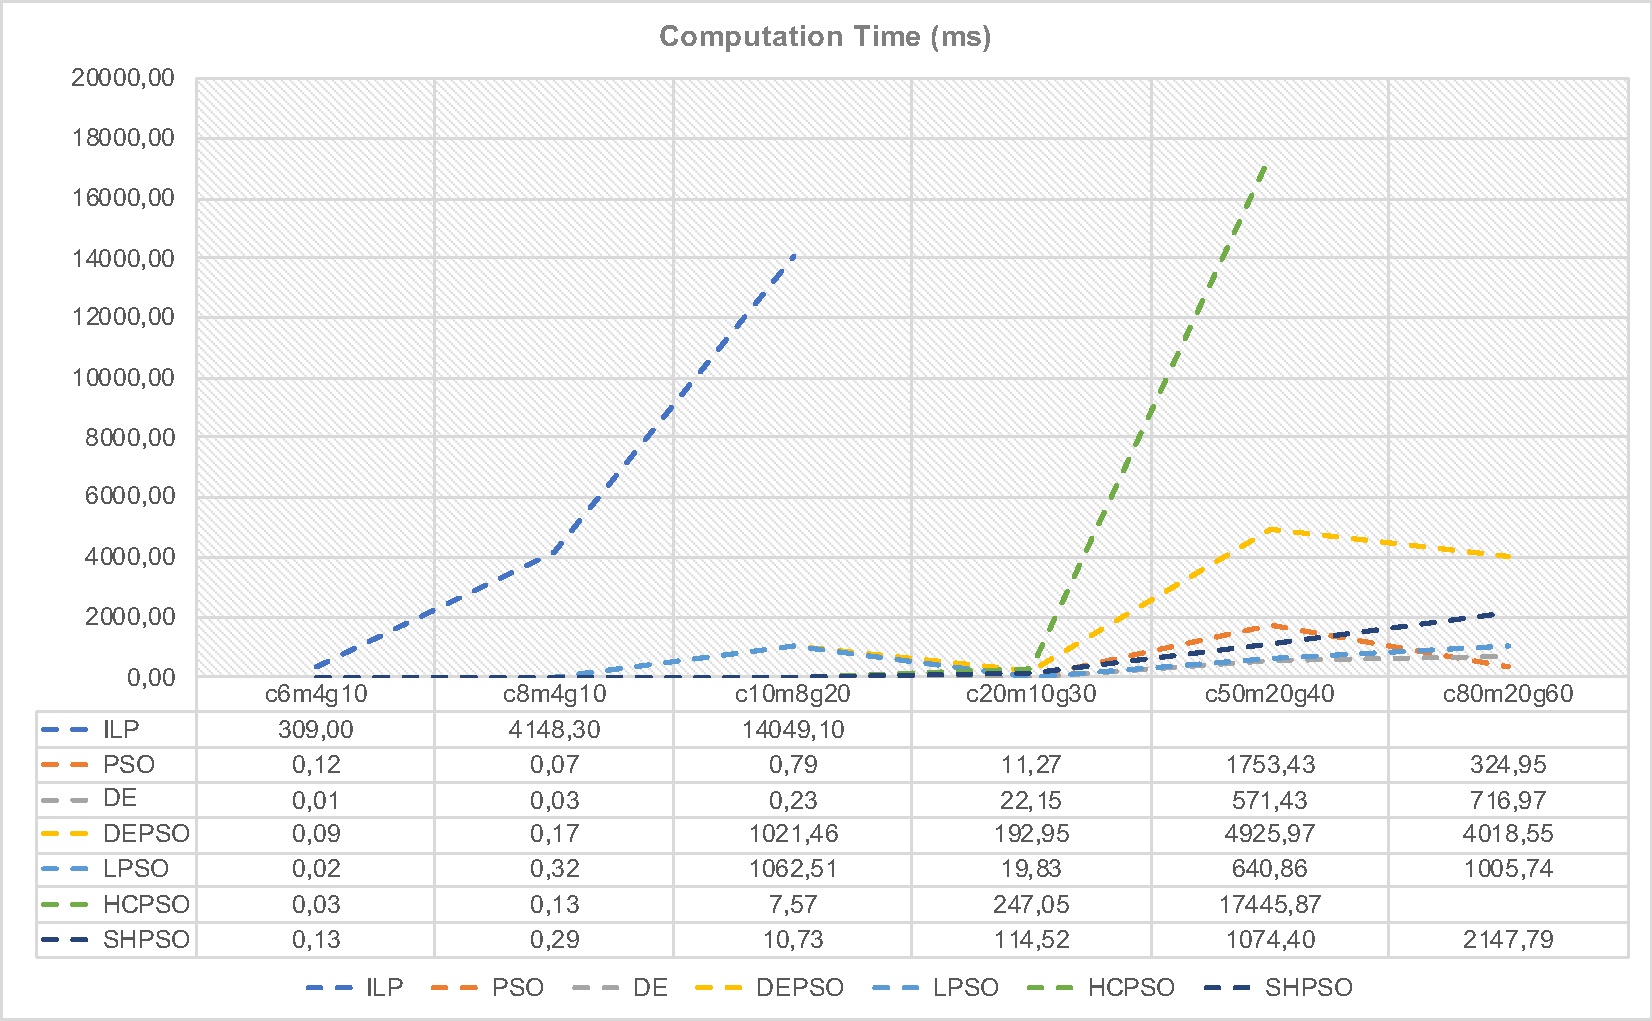
\includegraphics[width=0.9\linewidth]{images/time_summary.pdf}
	\caption{Computation time of the software allocation for different instances of the software allocation problems by different optimization algorithms.}
	\label{fig_allocationtime_ilp_metaheuristic}\vspace{-0.4cm}
\end{figure}

%Due to the replication of components to meet the reliability goals, the overhead of computing the delays is exponential. Figure~\ref{fig_chainsreplicationimprovements} compares the effect of with and without applying the approximation algorithm.  It shows that $61\%-81\%$ computation time improvement over the exact method while facing quality degradation only for samples $g_{30}d_{3}$ and  $g_{60}d_{2}$. The improvements are in seconds, which means for a single usage (or run) of the meta-heuristic optimization algorithms, it is not significant. However, considering practical engineering process, which requires several iterations, the commutative effect of applying the approximation algorithm can beneficial in terms of responsiveness to engineers. 
% \begin{figure}[h]
% 	\centering
% 	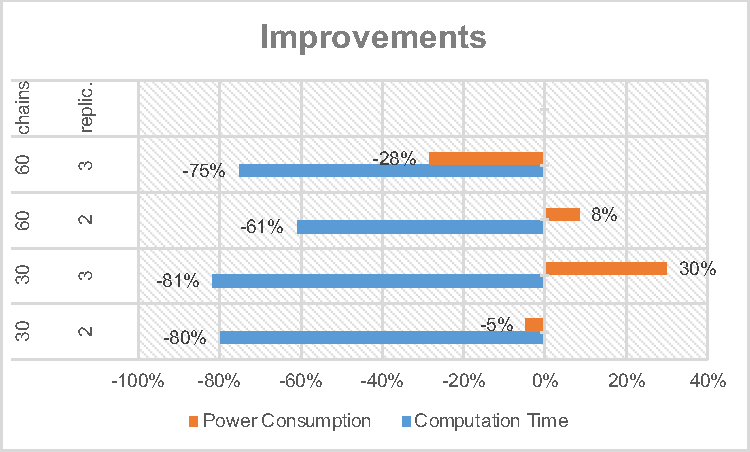
\includegraphics[width=0.7\linewidth]{images/chains_replication_improvements}
% 	\caption{Effect of approximate algorithm over delay calculations with replication.}
% 	\label{fig_chainsreplicationimprovements}
% \end{figure}

\section{Included Papers and their Mapping to Contributions and Goals}
\subsection*{Paper A}
ReSA: An ontology-based requirement specification language tailored to automotive systems. Nesredin~Mahmud, Cristina~Seceleanu and Oscar~Ljungkrantz.\textit{In the 10th IEEE International Symposium on Industrial Embedded Systems (SIES)(pp. 1-10). IEEE, 2015}.\label{lbl_resa}\\[6pt]
\textbf{Abstract:} \textit{Automotive systems are developed using multi-leveled architectural abstractions in an attempt to manage the increasing complexity and criticality of automotive functions. Consequently, well-structured and unambiguously specified requirements are needed on all levels of abstraction, in order to enable early detection of possible design errors. However, automotive industry often relies on requirements specified in ambiguous natural language, sometimes in large and incomprehensible documents. Semi-formal requirements specification approaches (e.g., requirement boilerplates, pattern-based specifications, etc.) aim to reduce requirements ambiguity, without altering their readability and expressiveness. Nevertheless, such approaches do not offer support for specifying requirements in terms of multi-leveled architectural concepts, nor do they provide means for early-stage rigorous analysis of the specified requirements. In this paper, we propose a language, called ReSA, which allows requirements specification at various levels of abstraction, modeled in the architectural language of EAST-ADL. ReSA uses an automotive systems' ontology that offers typing and syntactic axioms for the specification. Besides enforcing structure and more rigor in specifying requirements, our approach enables checking refinement as well as consistency of requirements, by proving ordinary boolean implications. To illustrate ReSA's applicability, we show how to specify some requirements of the Adjustable Speed Limiter, which is a complex, safety-critical Volvo Trucks user function.}\\[6pt]
\textbf{Personal Contributions: }I was the main driver of the paper. I developed the ReSA language including its syntax and semantics, and Cristina Seceleanu proposed a consistency analysis technique besides giving useful comments and ideas on the design of the language. Oscar Ljungkrantz provided useful materials from VGTT that were eventually analyzed for the language development, and gave feedback on the language design and implementation from an industrial viewpoint.\\
\textbf{Status:} Published

\subsection*{Paper B}
ReSA tool: Structured requirements specification and SAT-based consistency-checking. Nesredin~Mahmud, Cristina~Seceleanu and Oscar~Ljungkrantz. \textit{In the 2016 Federated Conference on Computer Science and Information Systems (FedCSIS)(pp. 1737-1746). IEEE, 2016.}\label{lbl_resatool}\\[6pt]
\textbf{Abstract:} \textit{Most industrial embedded systems requirements are
	specified in natural language, hence they can sometimes be
		ambiguous and error-prone. Moreover, employing an early-stage
		model-based incremental system development using multiple
		levels of abstraction, for instance via architectural languages
		such as EAST-ADL, calls for different granularity requirements
		specifications described with abstraction-specific concepts that
		reflect the respective abstraction level effectively.
		In this paper, we propose a toolchain for structured requirements
		specification in the ReSA language, which scales to multiple
		EAST-ADL levels of abstraction. Furthermore, we introduce
		a consistency function that is seamlessly integrated into the
		specification toolchain, for the automatic analysis of requirements
		logical consistency prior to their temporal logic formalization
		for full formal verification. The consistency check subsumes
		two parts: (i) transforming ReSA requirements specification into
		boolean expressions, and (ii) checking the consistency of the
		resulting boolean expressions by solving the satisfiability of their
		conjunction with the Z3 SMT solver. For validation, we apply
		the ReSA toolchain on an industrial vehicle speed control system,
		namely the Adjustable Speed Limiter.}\\[6pt]%abstract
	\textbf{Personal Contributions: }I was the main driver of the paper. I developed the ReSA toolchain that consists of the editor and the consistency checker including the integration with the Z3 SAT solver in the backend. Cristina Seceleanu formulated the consistency checking and together with Oscar Ljungkrantz, they contributed to the paper with useful comments and ideas.\\
		\textbf{Status: }Published

\subsection*{Paper C}
	Specification and semantic analysis of embedded systems requirements: From description logic to temporal logic. Nesredin~Mahmud, Cristina~Seceleanu and Oscar~Ljungkrantz. \textit{In the International Conference on Software Engineering and Formal Methods (SEFM)(pp. 332-348). Springer, Cham, 2017.}\label{lbl_resadl}\\[6pt]%authors
	\textbf{Abstract:} \textit{Due to the increasing complexity of embedded systems, early detection of software/hardware errors has become desirable. In this context, effective yet flexible specification methods that support rigorous analysis of embedded systems requirements are needed. Current specification methods such as pattern-based, boilerplates normally lack meta-models for extensibility and flexibility. In contrast, formal specification languages, like temporal logic, Z, etc., enable rigorous analysis, however, they usually are too mathematical and difficult to comprehend by average software engineers. In this paper, we propose a specification representation of requirements, which considers thematic roles and domain knowledge, enabling deep semantic analysis. The specification is complemented by our constrained natural language specification framework, ReSA, which acts as the interface to the representation. The representation that we propose is encoded in description logic, which is a decidable and computationally-tractable ontology language. By employing the ontology reasoner, Hermit, we check for consistency and completeness of requirements. Moreover, we propose an automatic transformation of the ontology-based specifications into Timed Computation Tree Logic formulas, to be used further in model checking embedded systems.}\\[6pt]%abstract
	\textbf{Personal Contributions:} I was the main driver of the language. I developed the ReSA language semantics using event-base approach, which is encoded in description logic. Cristina~Seceleanu and Ljungkrantz~Oscar provided with useful ideas and comments.\\
	\textbf{Status:} Published

\subsection*{Paper D}
SIMPPAAL - A Framework For Statistical Model Checking of Industrial Simulink Models. Predrag~Filipovikj, Nesredin~Mahmud, Raluca~Marinescu, Cristina~Seceleanu, Oscar~Ljungkrantz and Henrik~L\"{o}nn. \textit{Submitted to ACM Transactions on Software Engineering and Methodology (TOSEM).}\label{lbl_simulink_ilp}
\\[3pt]{\footnotesize This article is an extended version of the following conference paper:
     Simulink to UPPAAL Statistical Model Checker: Analyzing Automotive Industrial Systems.
Predrag Filipovikj, Nesredin Mahmud, Raluca Marinescu, Cristina Seceleanu, Oscar Ljungkrantz, Henrik L{\"o}nn. In Proceedings of the 21st International
Symposium on Formal Methods (FM2016), pages 748-756. Limassol, Cyprus. Springer, LNCS, November 2016. Revisions required. }\\[6pt]%authors
	\noindent \textbf{Abstract:} \textit{The evolution of automotive systems has been rapid. Nowadays, electronic brains control dozens of functions in vehicles, like
		braking, cruising, etc. Model-based design approaches, in environments such as MATLAB Simulink, seem to help in addressing
		the ever-increasing need to enhance quality, and manage complexity, by supporting functional design from a set of block
		libraries, which can be simulated and analyzed for hidden errors, but also used for code generation. For this reason, providing
		assurance that Simulink models fulfill given functional and timing requirements is desirable. In this paper, we propose a
		pattern-based, execution-order preserving automatic transformation of atomic and composite Simulink blocks into stochastic
		timed automata that can then be formally analyzed with Uppaal Statistical Model Checker (Uppaal SMC). To enable this, we
		first define the formal syntax and semantics of Simulink blocks and their composition, and show that the transformation is
		provably correct for a certain class of Simulink models. Our method is supported by the SIMPPAAL tool, which we introduce
		and apply on two industrial Simulink models, a prototype called the Brake-by-Wire and an operational Adjustable Speed
		Limiter system. This work enables the formal analysis of industrial Simulink models, by automatically generating stochastic
		timed automata counterparts.}\\[6pt]%abstract
	\textbf{Personal Contributions: } The three co-authors contributed equally to writing the paper. Technically, I equally contributed with proposing the pattern-based semantics of Simulink blocks, together with Predrag Filipovikj. I introduced a mechanism to enforce the execution order of the blocks using inter-arrival times. Predrag implemented the flattening algorithm and the tool for the automatic transformation of Simulink models into a network of timed automata with stochastic semantics. Raluca Marinescu contributed with analyzing the BBW system, Cristina Seceleanu contributed with defining the methodology, and with useful ideas and comments. Guillermo Rodriguez-Navas wrote the related work section. The industrial coauthors provided the use cases and commented on the final draft.\\
	\noindent\textbf{Status:} Revisions required. 

\subsection*{Paper E}
Power-aware Allocation of Fault-tolerant Multirate AUTOSAR Applications.
     Nesredin~Mahmud, Guillermo~Rodriguez-Navas, Hamid~Faragardi, Saad~Mubeen and Cristina~Seceleanu. \textit{In the 25th Asia-Pacific Software Engineering Conference (APSEC'18). IEEE.}  
     \label{lbl_softwareallocation_ilp}
\\[6pt]%authors
\textbf{Abstract:} \textit{The growing complexity of automotive functionality has attracted revolutionary computing architectures such as mixed-criticality design, which enables effective consolidation of software applications with different criticality on a shared execution platform. Mixed-critical design that is required to satisfy end-to-end timing and reliability specifications should consider power-efficient software design in order to accommodate more and more functionality. Due to the recursive and exhaustive nature of the real-time and reliability analysis, exact methods, e.g., branch and bound, dynamic programming, are prohibitively expensive. We propose hybrid particle-swarm optimization algorithms based on differential evolution and hill-climbing algorithms to minimize power consumption of the safety-critical software, which have end-to-end timing and reliability requirements, on a network of heterogeneous computing units. The optimization approach employs fault tolerance to maximize reliability of the software applications subsequently meet the reliability requirements. Our proposed integrated software-allocation approach is evaluated using a range of synthetic software applications based a real-world automotive benchmark. The evaluation makes comparative analysis of the differential evolution, particle-swarm optimization, integer-linear programming and hybrid particle-swarm optimization algorithms. The results show that the hybrid algorithms based on the hill-climbing algorithms outperform the rest of the meta-heuristic algorithms, in particular, the stochastic version of the hill-climbing algorithm scales well in large software allocation optimization problems while its overall optimality performance can be deemed acceptable.
}\\[6pt]%abstract
\textbf{My Contributions: } I was the main driver of the paper. I developed the system model with the guidance of the co-authors, and formulated the optimization problem with the guidance of Hamid~Faragardi, implemented the the problem in Java, and collected and analyzed the experimental results. The co-authors gave writing updates, useful ideas and comments on the paper, and specifically: Guillermo~Rodriguez-Navas on reliability analysis, Hamid~Faragardi on optimization, Saad~Mubeen on the timing analysis and Cristina~Seceleanu on the objective function and constraints.\\
\textbf{Status:} Published

\subsection*{Paper F}
Optimized Allocation of Fault-tolerant Embedded Software with End-to-end Timing Constraints.	\textit{M\"{a}lardalen Real-time Research Center Technical Report (MRTC), ISRN MDH-MRTC-325/2019-1-SE, 2019}. Submitted to Elsevier Journal of Systems Architecture (JSA).\\[6pt]%authors
\textbf{Abstract:} \textit{It is desirable to optimize power consumption of distributed safety-critical software that realize fault tolerance and maximize reliability as a result, to support the increasing complexity of software functionality in safety-critical embedded systems. Likewise, safety-critical applications that are required to meet end-to-end timing constraints may require additional computing resources. In this paper, we propose a scalable software-to-hardware allocation based on hybrid particle-swarm optimization with hill-climbing and differential algorithms to efficiently map software components to a network of heterogeneous computing nodes while meeting the timing and reliability constraints. The approach assumes fixed-priority preemptive scheduling, and delay analysis that value freshness of data, which is typical in control software applications.
Our proposed solution is evaluated on a range of software applications, which are synthesized from a real-world automotive AUTOSAR benchmark. The evaluation makes comparative analysis of the different algorithms, and a solution based on integer-linear programming, which is an exact method. The results show that the hybrid with the hill-climbing algorithms return very close solutions to the exact method and outperformed the hybrid with the differential algorithm, though consumes more time. The hybrid with the stochastic hill-climbing algorithm scales better and its optimality can be deemed acceptable.}\\[6pt]%abstract
\textbf{Personal Contributions: } I was the main driver of the paper. I developed the system model with the guidance of the co-authors, and formulated the optimization problem with the guidance of Hamid~Faragardi, implemented the the problem in Java, and collected and analyzed the experimental results. The co-authors gave writing updates, useful ideas and comments on the paper, and specifically: Guillermo~Rodriguez-Navas on reliability analysis, Hamid~Faragardi on optimization, Saad~Mubeen on the timing analysis and Cristina~Seceleanu on the objective function and constraints. \\%my contribution
\textbf{Status:} Submitted to Journal of System Architecture (JSA), Elsevier Journals.\\


In summary, the mapping between the included papers and the research contributions is given in Table~\ref{paper_contribution}, whereas the mapping between the research contributions and the research goals is given in Table~\ref{contribution_goals}.

% Please add the following required packages to your document preamble:
% \usepackage{booktabs}
\begin{table}[h!]
\centering
 \rowcolors{2}{gray!25}{white}
	\begin{tabular}{@{}ccccc@{}}
	%\rowcolor{gray!50}
		\toprule
		Paper & RC1 & RC2& RC3 & RC4\\ \midrule
		Paper A & $\times$ &  &  &  \\
		Paper B & $\times$ & $\times$ &  &  \\
		Paper C &  & $\times$ &  &  \\
		Paper D &  &  & $\times$  &\\
		Paper E &  &  &  & $\times$ \\
		Paper F &  &  &  & $\times$\\ \bottomrule
	\end{tabular}
\caption{Mapping between the included papers and the research contributions.}\label{paper_contribution}
\end{table}

% Please add the following required packages to your document preamble:
% \usepackage{booktabs}
\begin{table}[h!]
\centering
 \rowcolors{2}{gray!25}{white}
		\begin{tabular}{@{}cccccc@{}}
	%\rowcolor{gray!50}
		\toprule
		Contribution & RG1 & RG2& RG3 & RG4 & RG5\\ \midrule
		RC1 & $\times$ &  &  &  &$\times$\\
		RC2 &  & $\times$ &  & & $\times$\\
		RC3 &  &  & $\times$ & & $\times$\\
		RC4 &  &  &  & $\times$ &$\times$\\\bottomrule
	\end{tabular}
\caption{Mapping between the research contributions and the research goals.}\label{contribution_goals}
\end{table}

    \chapter{Research Method}
\label{methods}
Research methods, according to Jane et al. \cite{qualitateiveresearch2012}, are approaches, procedures and guidelines that are applied to conduct research, e.g., observation, interview, prototyping, experiment, etc. In this research, two main factors have driven the selection of research methods: i) the fact that the research is applied in industry (or involves industry-academia collaboration), which means the research results as well as the process should consider the interest and the nature of the industry, and ii) seamless integration of formal methods into existing engineering methods and practices with minimal cost, which requires careful consideration of existing engineering methods, guidelines, tools and capabilities. To summarize the main problems raised by the industry-academia collaboration: i) the research goals should target existing problems in the industry; ii) existing methods and tools should be leveraged; iii) proposed ideas, methods and tools should be agreed by both academia and industry teams before their design, implementation, validation, and integration to ensure usefulness; iv) furthermore, it is imperative that the proposed tools and methods are engineering-friendly, which means the research team is required to communicate with the actual users to capture the feel of the proposed methods and tools. 
\begin{figure}[h]
	\centering
	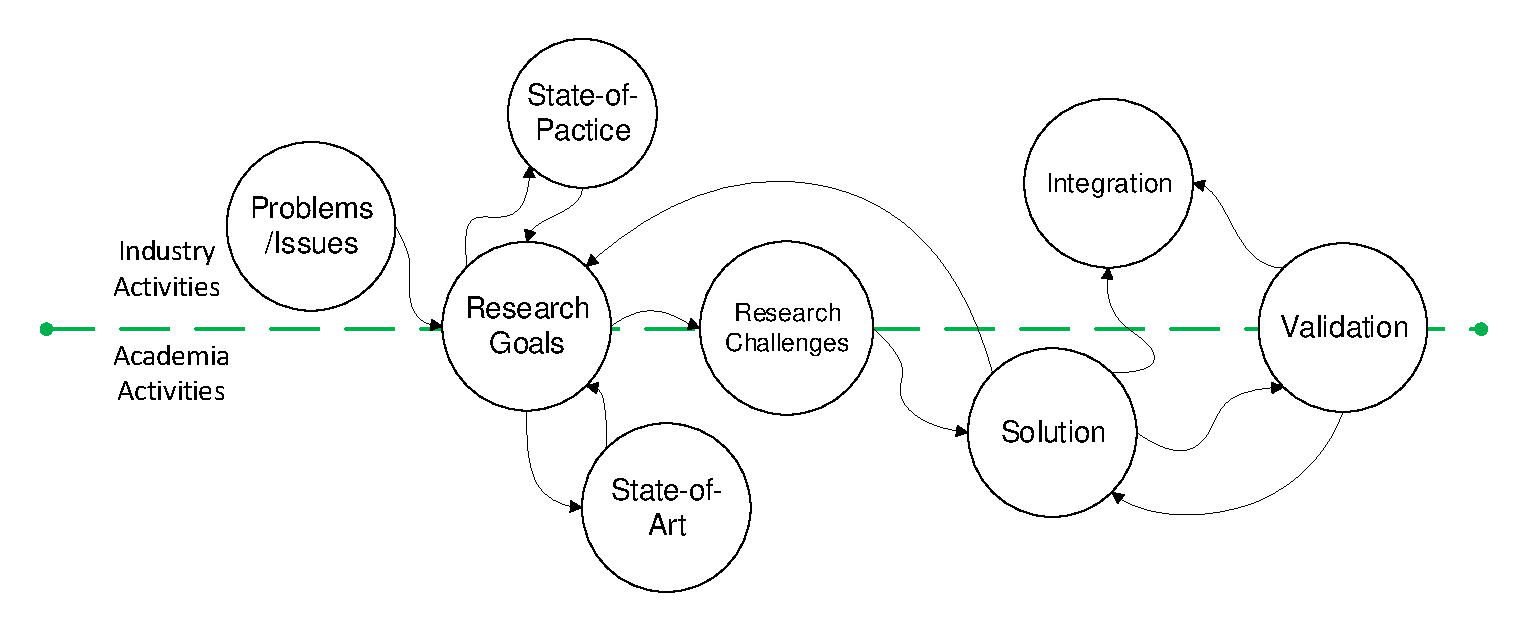
\includegraphics[trim=10 0 10 0, clip,width=1\linewidth]{images/research_process.pdf}
	\caption{Research Process.}
	\label{fig_research_process}
\end{figure}

Figure \ref{fig_research_process} illustrates the research process employed in the thesis, which is an adaptation of the technology-transfer process proposed by Tony et al. \cite{Gorschek2006APractice}. Our main research activities has involved identification of research goals and research challenges, which are followed by solution proposals and their implementations. Subsequently, the solutions are validated on industrial use cases, and are also integrated seamlessly into industrial tool chains. In order to conduct these activities, several quantitative and qualitative research methods are blended in order to gather, analyze and interpret, respectively, quantitative and qualitative data via what is known as \textit{hybrid (or mixed) research} \cite{Creswell2014ResearchApproaches}. The benefit of applying mixed research methods is mainly in the triangulation of research outcomes through various research methodical approaches. In fact, this can be better explained by the requirements specification research problem, which has accommodated empirical research via interview, observation to collect quantitative data that has allowed us to understand the current practices and needs of VGTT. Subsequently, we have proposed the ReSA framework, which have been validated through quantitative methods including statistical analysis and questionnaire on its effectiveness and usability\footnote{Work in progress - validation of the ReSA toolchain by practitioners, at VGTT.}.

During implementations of the proposed solutions, we have applied a prototyping method \cite{Carr2004PrototypingApproaches}, which has enabled incremental development of the solutions, before introducing grand progress in subsequent development phases, via concept modeling, implementation, demonstration and revision. This has been the case during the implementation of the ReSA framework \cite{resatool,Mahmud2017SpecificationLogic} as well as the SIMPPAAL framework \cite{Filipovikj2016SimulinkSystems}. The prototyping has involved concept development, and experimentation with toy examples and use cases to internally validate the implementation solutions, before validation by practitioners. Of course, the implementation of the research process has not been straightforward; on the contrary, similar to other research activities, it has accommodated several iterative, cyclic activities to clarify research goals and update solutions based on knowledge gained via literature study and feedback from industry.  Besides, the industrial flavor of the research has required persistent synchronization meetings through discussions and workshops in order to update to the state-of-the-art and state-of-the-practice methods and tools.
% \begin{figure} 
% \centering

%   	\includegraphics[trim=20 0 20 0, clip, width=0.7\linewidth]{research_method_activity.pdf}
%     \caption{Activity Diagram of the Research Process.}
%     \label{fig_discrete_block_ta}
%   \label{fig_ta}
% \end{figure}

    \chapter{Related Work}
    \chapter{Conclusions and Future Work}
In this thesis, we proposed formal methods and optimization techniques for the assured and efficient design of safety-critical embedded systems. We developed a domain-specific requirements specification language, i.e., \resa, which is tailored to embedded systems, and applied SAT-based and ontology-based techniques to improve quality of the specifications. Furthermore, we introduced an automated pattern-based, execution order-preserving method to transform large-scale Simulink models into networks of stochastic timed automata, which is analyzed by \uppaalsmc. For resource constrained design in general and low-battery embedded systems in particular, we propose efficient software allocation via integer linear programming and hybrid particle optimization on a network of heterogeneous computing nodes, i.e., with respect to power specification, failure rate and processor speed. During the allocation, the timing and the reliability constraints are satisfied by considering the worst case response time analysis, age delay analysis, and exact reliability analysis in the context of fault tolerance.

Our solution is validated on various industrial automotive use cases and benchmark. The requirements specification language is validated on the adjustable speed limiter (\asl) use case, the statistical model checking of Simulink models on the brake-by-wire (\bbw) use case, and the software allocation on the \autosar{} Benchmark produced Bosch. Our solution is effective, and scales well to large problems considering the following summery of observations: the SAT-based approach as opposed the ontology-based approach scales well. However, the analysis of the former is shallow due to abstraction of clauses whereas the latter is rigorous as it operates at the lexical level albeit scales less. We showed analysis of hybrid Simulink models via the stochastic time automata formalism, and its scalable analysis using the statistical model checking technique, i.e., on the \bbw{} model which consists of thousands of Simulink blocks. Finally, we showed that the ILP approach to software allocation scales only to 15 software components, and the population-based metaheuristics to very large applications, e.g., with 80 software components and 60 chains per application. Of the metaheuristic algorithms the hybrid \pso{} with hill climbing provided better quality solutions next to \ilp{} on small problems and performed best on larger problems. In particular the hybrid \pso{} with the stochastic hill climbing algorithm outperformed the rest for large software allocation problems.

Future work includes: (i) implementation of the ontology-based requirements analysis using open source lexical databases, e.g., WordNet; (ii) generalization of the statistical model checking to any data-flow programming paradigms; (iii) extend the software allocation problem to include dynamic synthesis of tasks; (iv) consider dynamic power consumption and extend the allocation to dynamic configuration of software components.

\backmatter

    % References
    % No restriction is set to the reference styles
    % Save your references in References.bib
    %\nocite{*} % Remove this for your own citations
    \bibliographystyle{plain}
    \bibliography{references}

\end{document}